\documentclass[]{article}
\usepackage[margin=1in]{geometry}
\usepackage{amsthm}
\usepackage{mathtools}
\usepackage{amsfonts}
\usepackage{multicol}
\usepackage{tikz}
\usepackage{eurosym}
\usepackage{algorithm}
\usepackage{algorithmicx}
\usepackage{algpseudocode}
\DeclareRobustCommand{\officialeuro}{%
	\ifmmode\expandafter\text\fi
	{\fontencoding{U}\fontfamily{eurosym}\selectfont e}}
\usepackage{caption}
\usepackage{subcaption}
\usetikzlibrary{matrix}
\usepackage{ stmaryrd }
\newtheorem{definition}{Definition}[section]
\newtheorem{theorem}{Theorem}[section]
\newtheorem{lemma}[theorem]{Lemma}
\usepackage[toc,page]{appendix}
\usepackage{forest}



%opening
\title{Verifying Featured Transition Systems using Variability Parity Games}
\author{Sjef van Loo}

\begin{document}

\maketitle

\tableofcontents

\part{Verifying featured transition systems}
\label{part:verifying}
\section{Introduction}
Model verification techniques can be used to improve the quality of software. These techniques require the behaviour of the software to be modelled, after which the model can checked to verify that it behaves conforming to some requirement. Different languages are proposed and well studied to express these requirements, examples are LTL, CTL, CTL* and $\mu$-calculus (TODO: cite). Once the behaviour is modelled and the requirement is expressed in some language we can use modal checking techniques to determine if the model satisfies the requirement.

These techniques are well suited to model and verify the behaviour of a single software product. However software systems can be designed to have certain parts enabled or disabled. This gives rise to many software products that all behave very similar but not identical, such a collection is often called a \textit{product family}. The differences between the products in a product family is called the \textit{variability} of the family. A family can be verified by using the above mentioned techniques to verify every single product independently. However this approach does not use the similarities in behaviour of these different products, an approach that would make use of the similarities could potentially be a lot more efficient.

\textit{Labelled transition systems} (LTSs) are often used to model the behaviour of a system, while it can model behaviour well it can't model variability. Efforts to also model variability include I/O automata, modal transition systems and \textit{featured transition systems} (FTSs) (TODO: cite). Specifically the latter is well suited to model all the different behaviours of the software products as well as the variability of the entire system in a single model.

Efforts have been made to verify requirements for entire FTSs, as well as to be able to reason about features. Notable contributions are fLTL, fCTL and fNuSMV (TODO: cite). However, as far as we know, there is no technique to verify an FTS against a $\mu$-calculus formula. Since the modal $\mu$-calculus is very expressive, it subsumes other temporal logics like LTL, CTL and CTL*, this is desired. In this thesis we will introduce a technique to do this. We first look at LTSs, the modal $\mu$-calculus and FTSs. Next we will look at an existing technique to verify an LTS, namely solving \textit{parity games}, as well as show how this technique can be used to verify an FTS by verifying every software product it describes independently. An extension to this technique is then proposed, namely solving \textit{variability parity games}. We will formally define variability parity games and prove that solving them can be used to verify FTSs.

\section{Verifying transition systems}
We first look at labelled transition systems (LTSs) and the modal $\mu$-calculus and what it means to verify an LTS. The definition below are derived from \cite{Groote}.
\begin{definition}
	\label{def_lts}A labelled transition system (LTS) is a tuple $M = (S, Act, trans, s_0)$, where:
	\begin{itemize}
		\item $S$ is a set of states,
		\item $Act$ a set of actions,
		\item $trans \subseteq S \times Act \times S$ is the transition relation with $(s,a,s') \in trans$ denoted by $s \xrightarrow a s'$,
		\item $s_0 \in S$ is the initial state.
	\end{itemize}
\end{definition}
Consider the example in figure \ref{fig:coffeemachinebasiceurolts} (directly taken from \cite{FamBasedModelCheckingWithMCRL2}) of a coffee machine where we have two actions: ins (insert coin) and std (get standard sized coffee).\\
\begin{figure}[h]
	\centering
	\includegraphics[scale=0.5]{Examples/CoffeeMachine/BasicEuroLTS}
	\caption[Coffee machine LTS]{Coffee machine LTS $C$}
	\label{fig:coffeemachinebasiceurolts}
\end{figure}


\begin{definition}
	\label{def_mu_syntax}
	A modal $\mu$-calculus formula over the set of actions $Act$ and a set of variables $\mathcal{X}$ is defined by
	\[ \varphi = \top\ |\ \bot\ |\ X\ |\ \varphi \vee \varphi\ |\ \varphi \wedge \varphi\ |\ \langle a \rangle \varphi\ |\ [a]\varphi\ |\ \mu X.\varphi\ |\ \nu X.\varphi \]
	with $a \in Act$ and $X \in \mathcal{X}$. 
	
	
	No negations in the language because negations can be pushed inside to the propositions, ie. the $\top$ and $\bot$ elements.
\end{definition}
The modal $\mu$-calculus contains boolean constants $\top$ and $\bot$, propositional operators $\vee$ and $\wedge$, modal operators $\langle \, \rangle$ and $[ \, ]$ and fixpoint operators $\mu$ and $\nu$. A formula is closed when variables only occur in the scope of a fixpoint operator for that variable.

A modal $\mu$-calculus formula can be interpreted with an LTS, this results in a set of states for which the formula holds.
\begin{definition}
	\label{def_mu_sem} For LTS $(S, Act, trans, s_0)$ we inductively define the interpretation of a modal $\mu$-calculus formula $\varphi$, notation
	$[\![ \varphi ]\!]^\eta$, where $\eta : \mathcal{X} \rightarrow \mathcal{P}(S)$ is a logical variable valuation, as a set of states
	where $\varphi$ is valid, by:
	\begin{align*}
	&[\![ \mathit{\top} ]\!]^\eta &&= S\\
	&[\![ \mathit{\bot} ]\!]^\eta &&= \emptyset\\
	&[\![ \varphi_1 \wedge \varphi_2 ]\!]^\eta &&= [\![ \varphi_1 ]\!]^\eta \cap [\![ \varphi_2 ]\!]^\eta \\
	&[\![ \varphi_1 \vee \varphi_2 ]\!]^\eta &&= [\![ \varphi_1 ]\!]^\eta \cup [\![ \varphi_2 ]\!]^\eta\\
	&[\![ \langle a \rangle \varphi ]\!]^\eta &&= \{s \in S|\exists_{s' \in S} s \xrightarrow {a} s' \wedge s' \in [\![ \varphi ]\!]^\eta\}\\
	&[\![ [ a ] \varphi ]\!]^\eta &&= \{s \in S|\forall_{s' \in S} s \xrightarrow {a} s' \implies s' \in [\![ \varphi ]\!]^\eta\}\\
	&[\![ \mu X. \varphi ]\!]^\eta &&= \bigcap_{f \subseteq S}\{f | f = [\![ \varphi ]\!]^{\eta[X:=f]}\}\\
	&[\![ \nu X. \varphi ]\!]^\eta &&= \bigcup_{f \subseteq S}\{f | f = [\![ \varphi ]\!]^{\eta[X:=f]}\}\\
	&[\![ X ]\!]^\eta &&= \eta(X)
	\end{align*}
\end{definition}

Given closed formula $\varphi$, LTS $M = (S, Act, trans, s_0)$ and $s \in S$ we write $(M,s) \models \varphi$ iff $s \in [\![ \varphi ]\!]^\eta$ for $M$, we say that formula $\varphi$ holds for $M$ in state $s$. If formula $\varphi$ holds for $M$ in the initial state we say that formula $\varphi$ holds for $M$ and write $M \models \varphi$.

Again consider the coffee machine example (figure \ref{fig:coffeemachinebasiceurolts}) and formula $\varphi = \nu X. \mu Y. ([ins]Y \wedge [std] X)$ (taken from \cite{FamBasedModelCheckingWithMCRL2}) which states that action std must occur infinitely often over all runs. Obviously this holds for the coffee machine, therefore we have $C \models \varphi$.

\subsection{Featured transition systems}
A featured transition system extends the LTS definition to express variability. It does so by introducing \textit{features} and \textit{products} into the definition. Features are options that can be enabled or disabled for the system. A product is a feature assignments, ie. a set of features that is enabled for that product. Not a products are valid, some features might be mutually exclusive and some features might always be required. To express products one can use feature diagrams as explained in \cite{Classen2013FeaturedTS}. Feature diagrams offer a nice way of expressing which feature assignments are valid, but since they offer just that we simply represent the valid products with a set of feature assignments. Finally FTSs guards every transition with a boolean expression over the set of features. We have the following definition, based on \cite{Classen2013FeaturedTS}:
\begin{definition}
	\label{def_fts}A featured transition system (FTS) is a tuple $M = (S, Act, trans, s_0, N, P, \gamma)$, where:
	\begin{itemize}
		\item $S, Act, trans, s_0$ are defined as in an LTS,
		\item $N$ is a non-empty set of features,
		\item $P \subseteq \mathcal{P}(N)$ is a set of products, ie. feature assignments, that are valid,
		\item $\gamma : trans \rightarrow \mathbb{B}(N)$ is a total function, labelling each transition with a boolean expression over the features. A product $p \in \mathcal{P}(N)$ satisfying the boolean expression of transition $t$ is denoted by $p \models \gamma(t)$, $\gamma(t)(p) = 1$ or $p \in [\![\gamma(t)]\!]$. The boolean expression that is satisfied by any feature assignment is denoted by $\top$, ie $p \models \top$ for any $p$.
		
		A transition $s \xrightarrow a s'$ and $\gamma((s,a,s')) = f$ is denoted by $s \xrightarrow {a | f} s'$. 
	\end{itemize}
\end{definition}
\begin{figure}[h]
\centering
\includegraphics[scale=0.5]{Examples/CoffeeMachine/FTS}
\caption[Coffee machine LTS]{Coffee machine FTS $C$}
\label{fig:coffeemachinefts}
\end{figure}

Consider the example in figure \ref{fig:coffeemachinefts} (directly taken from \cite{FamBasedModelCheckingWithMCRL2}) which shows an FTS for a coffee machine For this example we have two features $N = \{\$, \officialeuro\}$ and two valid products $P = \{\{\$\},\{\officialeuro\}\}$.

An FTS expresses they behaviour of multiple products, we can derive the behaviour of a single product by simply removing all the transitions from the FTS for which the product doesn't satisfy the feature expression guarding the transition. We call this a \textit{projection} (\cite{Classen2013FeaturedTS}).

\begin{definition}
	\label{def_fts_proj}
	The projection of an FTS $M = (S, Act, trans, s_0, N, P, \gamma)$ to a product $p \in P$, noted $M_{|p}$, is the LTS $M'=(S,Act,trans', s_0)$, where $trans' = \{t \in trans\ |\ p \models \gamma(t)\}$.
\end{definition}
The coffee machine example can be projected to its two products, which results in the LTSs in figure \ref{fig:cofeemachineftsproj}.
\begin{figure}[h]
	\centering
	\begin{subfigure}{.5\textwidth}
		\centering
		\includegraphics[width=1\linewidth]{Examples/CoffeeMachine/FTSProjDollar}
		\caption[$C_{|\{\$\}}$]{$C$ projected to the dollar product: $C_{|\{\$\}}$}
		\label{fig:coffeemachineftsprojdollar}
	\end{subfigure}%
	\begin{subfigure}{.5\textwidth}
		\centering
		\includegraphics[width=1\linewidth]{Examples/CoffeeMachine/FTSProjEuro}
		\caption[$C_{|\{\$\}}$]{$C$ projected to the euro product: $C_{|\{\officialeuro\}}$}
		\label{fig:coffeemachineftsprojeuro}
	\end{subfigure}
	\caption{Projections of the coffee machine FTS}
	\label{fig:cofeemachineftsproj}
\end{figure}

We want to verify the FTS against a modal $\mu$-calculus formula $\varphi$. That is, we want to find out for which products in the FTS its projection satisfies $\varphi$. Formally, given FTS $M = (S, Act, trans, s_0, N, P, \gamma)$ and modal $\mu$-calculus formula $\varphi$ we want to find $P_s \subseteq P$ such that:
\begin{itemize}
	\item for every $p \in P_s$ we have $M_{|p} \models \varphi$ and
	\item for every $p \in P \backslash P_s$ we have $M_{|p} \not\models \varphi$.
\end{itemize}
Furthermore a counterexample for every $p \in P \backslash P_s$ is preferred.

\section{Verification using parity games}
Verifying LTSs against a modal $\mu$-calculus formula can be done by solving a parity game. This is done by translating an LTS in combination with a formula to a parity game, the solution of the parity game provides the information needed to conclude if the model satisfies the formula. This relation is depicted in figure \ref{fig:ltsverificationusingpg}. This technique is well known and well studied, in this section we will first look at parity games, the translation from LTS and formula to a parity game and finally what we can do with this technique to verify FTS.
\begin{figure}[h]
	\centering
	\includegraphics[scale=0.5]{Diagrams/LTSVerificationUsingPG}
	\caption[LTS verification using PG]{LTS verification using PG}
	\label{fig:ltsverificationusingpg}
\end{figure}

\subsection{Parity games}
\begin{definition}
	\label{def_PG}\cite{Bradfield2018}
	A parity game (PG) is a tuple $(V, V_0, V_1, E, \rho)$, where:
	\begin{itemize}
		\item $V = V_0 \cup V_1$ and $V_0 \cap V_1 = \emptyset$,
		\item $V_0$ is the set of vertices owned by player $0$,
		\item $V_1$ is the set of vertices owned by player $1$, 
		\item $E \subseteq V \times V$ is the edge relation,
		\item $\rho :  V \rightarrow \mathbb{N}$ is a priority assignment.
	\end{itemize}
\end{definition}
We write $\alpha \in \{0,1\}$ to denote an arbitrary player. We write $\overline{\alpha}$ to denote $\alpha$'s opponent, ie. $\overline{0} = 1$ and $\overline{1} = 0$.

A parity game is played by players 0 and 1. A play starts with placing a token on vertex $v \in V$. Player $\alpha$ moves the token if the token is on a vertex owned by $\alpha$, ie. $v \in V_\alpha$. The token can be moved to $w \in V$, with $(v,w) \in E$. A series of moves results in a sequence of vertices, called path. For path $\pi$ we write $\pi_i$ to denote the $i^{\text{th}}$ vertex in path $\pi$. A play ends when the token is on vertex $v \in V_\alpha$ and $\alpha$ can't move the token anywhere, in this case player $\overline{\alpha}$ wins the play. If the play results in an infinite path $\pi$ then we determine the highest priority that occurs infinitely often in this path, formally
\[ \max\{ p \ |\ \forall_j \exists_i j < i \wedge p = \rho(\pi_i) \}\] 
If the highest priority is odd then player $1$ wins, if it is even player $0$ wins.
\begin{figure}[h]
	\centering
	\includegraphics[scale=0.3]{Examples/SimplePG/PG}
	\caption[Parity game example]{Parity game example}
	\label{fig:simplepgpg}
\end{figure}

Figure \ref{fig:simplepgpg} shows an example of a parity game. We usually depict the vertices owned by player $0$ by diamonds and vertices owned by player $1$ by boxes, the priority is depicted inside the vertices. If the game starts by placing a token on $v_1$ we can consider the following exemplary paths:
\begin{itemize}
	\item $\pi = v_1v_3v_5$ is won by player $1$ since player $0$ can't move at $v_5$.
	\item $\pi = (v_1v_2)^\omega$ is won by player $1$ since the highest priority occurring infinitely often is 3.
	\item $\pi = v_1v_3(v_4)^\omega$ is won by player $0$ since the highest priority occurring infinitely often is $0$.
\end{itemize}


A strategy for player $\alpha$ is a function $\sigma : V^*V_\alpha \rightarrow V$ that maps a path ending in a vertex owned by player $\alpha$ to the next vertex. Parity games are positionally determined \cite{Bradfield2018}, therefore a strategy $\sigma: V_\alpha \rightarrow V$ that maps the current vertex to the next vertex is sufficient. 

A strategy $\sigma$ for player $\alpha$ is winning from vertex $v$ if and only if any play that results from following $\sigma$ results in a win for player $\alpha$. The graph can be divided in two partitions $W_0 \subseteq V$ and $W_1 \subseteq V$, called winning sets. If and only if $v \in W_\alpha$ then player $\alpha$ has a winnings strategy from $v$. Every vertex in the graph is either in $W_0$ or $W_1$ \cite{Bradfield2018}. Furthermore finite parity games are decidable \cite{Bradfield2018}.
\subsection{Creating parity games}

\subsection{FTSs and parity games}

\section{Featured parity games}







Before we can define variability parity games we first define \textit{featured parity games} (FPG), featured parity games extend the definition of parity games to capture the variability represented in an FTS. It uses the same concepts as FTSs: features, products and a function that guards edges. In this section we will introduce the definition of FPGs and show that solving them answers the verification questions for FTS: For which products in the FTS does its projection satisfy $\varphi$?

First we introduce the definition of an FPG:
\begin{definition}
	\label{def_FPG}
	A featured parity game (FPG) is a tuple $(V,V_0, V_1, E, \Omega, N, P, \gamma)$, where:
	\begin{itemize}
		\item $V = V_0 \cup V_1$ and $V_0 \cap V_1 = \emptyset$,
		\item $V_0$ is the set of vertices owned by player $0$,
		\item $V_1$ is the set of vertices owned by player $1$, 
		\item $E \subseteq V \times V$ is the edge relation,
		\item $\Omega :  V \rightarrow \mathbb{N}$ is a priority assignment,
		\item $N$ is a non-empty set of features,
		\item $P \subseteq \mathcal{P}(N)$ is a non-empty set of products, ie. feature assignments, for which the game can be played,
		\item $\gamma : E \rightarrow \mathbb{B}(N)$ is a total function, labelling each edge with a Boolean expression over the features.
	\end{itemize}
\end{definition}
An FPG is played similarly to a PG, however the game is played for a specific product $p \in P$. Player $\alpha$ can only move the token from $v \in V_\alpha$ to $w \in V$ if $(v,w) \in E$ and $p \models \gamma(v,w)$.

A game played for product $p \in P$ results in winnings sets $W_0^p$ and $W_1^p$, which are defined similar to the $W_0$ and $W_1$ winning sets for parity games.

An FPG can simply be projected to a product $p$ by removing the edges that are not satisfied by $p$.
\begin{definition}
	\label{def_FPG_proj}
	The projection from FPG $G = (V,V_0, V_1, E, \Omega, N, P, \gamma)$ to a product $p \in P$, noted $G_{|p}$, is the parity game $(V,V_0,V_1, E', \Omega)$ where $E' = \{ e \in E\ |\ p \models \gamma(e) \}$.
\end{definition}

Playing FPG $G$ for a specific product $p\in P$ is the same as playing the PG $G_{|p}$. Any path that is valid in $G$ for $p$ is also valid in $G_{|p}$ and vice versa. Therefore the strategies are also interchangeable, furthermore the winning sets $W_\alpha$ for $G_{|p}$ and $W_\alpha^p$ for $G$ are identical. Since parity games are positionally determined so are FPGs. Similarly, since finite parity games are decidable, so are finite FPGs.

We say that an FPG is solved when the winning sets for every valid product in the FPG are determined.
\subsubsection{Creating featured parity games}
An FPG can be created from an FTS in combination with a model $\mu$-calculus formula. We translate an FTS to an FPG by first creating a PG from the transition system as if there were no transition guards, next we apply the same guards to the FPG as are present in the FTS for edges that originate from transitions. The features and valid products in the FPG are identical to those in the FTS.
\begin{definition}
	\label{def_FTS2FPG}
	$FTS2FPG(M, \varphi)$ converts FTS $M = (S, Act, trans, s_0, N, P, \gamma)$ and closed formula $\varphi$ to FPG $(V, V_0, V_1, E, \Omega, N, P, \gamma')$.
	
	We have $(V, V_0, V_1, E, \Omega) = \textit{LTS2PG}((S, Act, trans, s_0), \varphi$) and
	\[ \gamma'((s, \psi),(s', \psi')) = \begin{cases}
	\gamma(s,a,s') & \text{if }\psi = \langle a \rangle \psi'\text{ or }\psi = [a]\psi' \\
	\top & \text{otherwise}
	\end{cases}\]
\end{definition}
Consider our working example which we extend to an FTS depicted in figure \ref{fig:exverfts}, for this example we have features $N = \{f, g\}$ and products $P = \{\emptyset, \{f\},\{f,g\}\}$.

\begin{figure}[h]
	\centering
	\includegraphics[scale=0.3]{Examples/ExamleVerification/FPG}
	\caption[FPG for $M$ and $\varphi$]{FPG for $M$ and $\varphi$}
	\label{fig:exverfpg}
\end{figure}
We can translate this FTS with formula $\varphi = \mu X. ([a] X \vee \langle b \rangle \top)$ to an FPG depicted in figure \ref{fig:exverfpg}. As we can see from the FTS if feature $f$ is enabled and $g$ is disabled then we have an infinite path of $a$'s where $b$ is never enabled, therefore $\varphi$ doesn't hold for $M_{|\{f\}}$. If $g$ is enabled however we can always do a $b$ so $\varphi$ holds for $M_{|\{f,g\}}$. As we have seen $\varphi$ does hold for $M_{|\emptyset}$. For the product $\emptyset$ we have the same winning set as before:
\begin{align*}
W_0^\emptyset = \{& (s_1, \mu X.\phi),\\
& (s_1, [a](\mu X.\phi) \vee \langle b \rangle \top),\\
& (s_1, [a](\mu X.\phi)),\\
& (s_1, \top),\\
& (s_2, \mu X.\phi),\\
& (s_2, [a](\mu X.\phi) \vee \langle b \rangle \top),\\
& (s_2, [a](\mu X.\phi)),\\
& (s_2, \langle b \rangle \top),\\
& (s_2, \top)
\}\\
W_1^\emptyset = \{& (s_1, \langle b \rangle \top )\}
\end{align*}
In the FPG we can see that if $f$ is enabled and $g$ is disabled then player $1$ can move the token from $(s_1, [a]X)$ to $(s_1,X)$. This results in player $0$ either moving the token to $(s_1, \langle b \rangle \top)$ and losing or an infinite path where $1$ occurs infinitely often which is also player $1$ wins. For product $\{f\}$ we have winning sets:
\begin{align*}
W_0^{\{f\}} = \{
& (s_1, \top),\\
& (s_2, \mu X.\phi),\\
& (s_2, [a](\mu X.\phi) \vee \langle b \rangle \top),\\
& (s_2, \langle b \rangle \top),\\
& (s_2, \top)
\}\\
W_1^{\{f\}} = \{& (s_1, \mu X.\phi),\\
& (s_1, [a](\mu X.\phi) \vee \langle b \rangle \top),\\
& (s_1, [a](\mu X.\phi)),\\
& (s_1, \langle b \rangle \top ),\\
& (s_2, [a](\mu X.\phi))\}
\end{align*}
However if $g$ is also enabled then player $0$ wins in $(s_1, \langle b \rangle \top)$, thus giving the following winning sets:
\begin{align*}
W_0^{\{f,g\}} = \{& (s_1, \mu X.\phi),\\
& (s_1, [a](\mu X.\phi) \vee \langle b \rangle \top),\\
& (s_1, [a](\mu X.\phi)),\\
& (s_1, \langle b \rangle \top ),\\
& (s_1, \top),\\
& (s_2, \mu X.\phi),\\
& (s_2, [a](\mu X.\phi) \vee \langle b \rangle \top),\\
& (s_2, [a](\mu X.\phi)),\\
& (s_2, \langle b \rangle \top),\\
& (s_2, \top)
\}\\
W_1^{\{f,g\}} = \{\}
\end{align*}

In the next section we will show how the winning sets relate to the model verification question.


\subsubsection{FTS verification using featured parity games}
We can create an FPG from an FTS and project it to a product, resulting in a PG, this is shown in the following diagram:\\
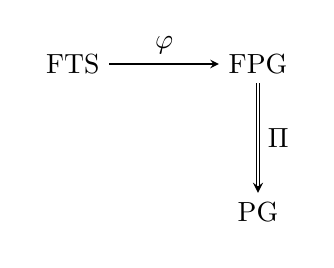
\begin{tikzpicture}
\matrix (m) [matrix of math nodes,row sep=4em,column sep=4em,minimum width=2em]
{
	\text{FTS} & \text{FPG} \\
	\  & \text{PG} \\};
\path[-stealth]
(m-1-1)
edge node [above] {$\varphi$} (m-1-2)

(m-1-2) edge [double] node [right] {$\Pi$} (m-2-2)
;
\end{tikzpicture}\\
Earlier we saw that we could also derive a PG by projecting the FTS to a product and then translation the resulting LTS to a PG, depicted by the following diagram:
\\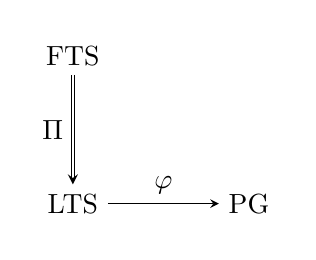
\begin{tikzpicture}
\matrix (m) [matrix of math nodes,row sep=4em,column sep=4em,minimum width=2em]
{
	\text{FTS} \\
	\text{LTS} & \text{PG} \\};
\path[-stealth]
(m-1-1) edge [double] node [left] {$\Pi$} (m-2-1)
(m-2-1.east|-m-2-2) edge node [above] {$\varphi$}
(m-2-2)
;
\end{tikzpicture}\\
We will now show that the resulting parity games are identical.
\begin{theorem}
	\label{the_PGsubPGA} Given:
	\begin{itemize}
		\item FTS $M = (S,Act, trans, s_0, N, P, \gamma)$,
		\item a closed modal mu-calculus formula $\varphi$,
		\item a product $p \in P$
	\end{itemize}
	it holds that the parity games LTS2PG($M_{|p}, \varphi$) and FTS2FPG($M, \varphi$)$_{|p}$  are identical.
	\begin{proof}
		Let $G^F = (V^F, V_0^F, V_1^F, E^F, \Omega^F, N, P, \gamma') = FTS2FPG(M, \varphi)$, using definition \ref{def_FTS2FPG}, and $G^F_{|p} = (V^F, V_0^F, V_1^F, {E^F}', \Omega^F)$, using definition \ref{def_FPG_proj}. Furthermore we have $M_{|p} = (S, Act, trans', s_0)$ and we let $G = (V, V_0, V_1, E, \Omega) =  LTS2PG(M_{|p}, \varphi)$. We depict the different transition systems and games in the following diagram.
		
		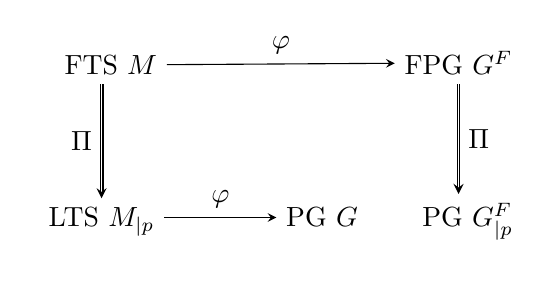
\begin{tikzpicture}
		\matrix (m) [matrix of math nodes,row sep=4em,column sep=1em,minimum width=2em]
		{
			\text{\ \ FTS }M & \  &\ & \text{FPG } G^F  \\
			\text{LTS }M_{|p} & \ & \text{PG } G & \text{\ \ PG }G_{|p}^F \\};
		\path[-stealth]
		(m-1-1) edge [double] node [left] {$\Pi$} (m-2-1)
		edge node [above] {$\varphi$} (m-1-4)
		(m-2-1.east|-m-2-3) edge node [above] {$\varphi$}
		(m-2-3)
		(m-1-4) edge [double] node [right] {$\Pi$} (m-2-4);
		\end{tikzpicture}\\
		We will prove that $G = G_{|p}^F$. We first note that game $G$ is created by 
		\[  (V, V_0, V_1, E, \Omega) = LTS2PG((S, Act, trans', s_0),\varphi) \]
		and the vertices, edges and priorities of game $G^F$ are created by 
		\[ (V^F, V_0^F, V_1^F, E^F, \Omega^F) = LTS2PG((S,Act, trans, s_0), \varphi)\]
		Using the definition of LTS2PG (\ref{def_LTS2PG}) we find that the vertices and the priorities only depend on the states in $S$ and the formula $\varphi$, since these are identical in the above two statements we immediately get $V = V^F, V_0 = V_0^F, V_1 = V_1^F$ and $\Omega = \Omega^F$. The vertices and priorities don't change when an FTS is projected, therefore $G_{|p}^F$ has the same vertices and priorities as $G^F$.
		
		Now we are left with showing that $E = {E^F}'$ in order to conclude that that $G = G^F_{|p}$. We will do this by showing $E \subseteq {E^F}'$ and $E \supseteq {E^F}'$.
		
		First let $e \in E$. Note that a vertex in the parity game is represented by a pair of a state and a formula. So we can write $e = ((s,\psi),(s',\psi'))$. To show that $e \in {E^F}'$ we distinguish two cases:
		\begin{itemize}
			\item  If $\psi = \langle a \rangle \psi'$ or $\psi = [a] \psi'$ then there exists an $a \in Act$ such that $(s,a,s') \in trans'$. Using the FTS projection definition (\ref{def_fts_proj}) we get $(s,a,s') \in trans$ and $p \models \gamma(s,a,s')$. Using the FTS2FPG definition (\ref{def_FTS2FPG}) we find that $\gamma'((s,\psi),(s',\psi')) = \gamma(s,a,s')$ and therefore $p \models \gamma'((s,\psi),(s',\psi'))$. Now using the FPG projection definition (\ref{def_FPG_proj}) we find $((s,\psi),(s',\psi')) \in {E^F}'$.
			\item Otherwise the existence of the edge does not depend on the $trans$ parameter and therefore $((s,\psi),(s',\psi')) \in {E^F}'$ if $(s,\psi) \in V^F$, since $V^F = V$ we have $(s,\psi) \in V^F$.
		\end{itemize}
		We can conclude that $E \subseteq {E^F}'$, next we will show $E \supseteq {E^F}'$. Let $e = ((s,\psi),(s',\psi')) \in {E^F}'$. We distinguish two cases:
		\begin{itemize}
			\item If $\psi = \langle a \rangle \psi'$ or $\psi = [a] \psi'$ then there exists an $a \in Act$ such that $(s,a,s') \in trans$. Using the FPG projection definition (\ref{def_FPG_proj}) we get $p \models \gamma'(s,a,s')$. Using the FTS2FPG definition (\ref{def_FTS2FPG}) we get $p \models \gamma(s,a,s')$. Using the FTS projection definition (\ref{def_fts_proj}) we get $(s,a,s') \in trans'$ and therefore $((s,\psi),(s',\psi'))\in E$.
			\item Otherwise the existence of the edge does not depend on the $trans$ parameter and therefore $((s,\psi),(s',\psi')) \in E$ if $(s,\psi) \in V$, since $V^F = V$ we have $(s,\psi) \in V$.
		\end{itemize}
	\end{proof}
\end{theorem}

Having proven this we can visualize the relation between the different games and transition systems in the following diagram:
\\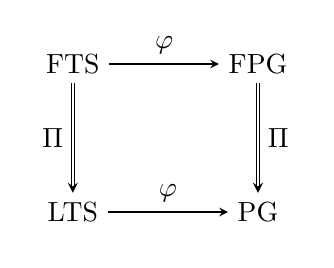
\begin{tikzpicture}
\matrix (m) [matrix of math nodes,row sep=4em,column sep=4em,minimum width=2em]
{
	\text{FTS} & \text{FPG} \\
	\text{LTS} & \text{PG} \\};
\path[-stealth]
(m-1-1) edge [double] node [left] {$\Pi$} (m-2-1)
edge node [above] {$\varphi$} (m-1-2)
(m-2-1.east|-m-2-2) edge node [above] {$\varphi$}
(m-2-2)
(m-1-2) edge [double] node [right] {$\Pi$} (m-2-2)
;
\end{tikzpicture}\\
Finally we prove that solving an FTS, ie. finding winning sets for all products, answers the verification question.
\begin{theorem}
	\label{the_FPG_ver_FTS}
	Given:
	\begin{itemize}
		\item FTS $M = (S, Act, trans, s_0, N, P, \gamma)$,
		\item closed modal mu-calculus formula $\varphi$,
		\item product $p \in P$ and
		\item state $s \in S$
	\end{itemize}
	it holds that $(M_{|p}, s) \models \varphi$ if and only if $(s, \varphi) \in W_0^p$ in $\textit{FTS2FPG}(M, \varphi$).
	\begin{proof}
		The winning set $W_\alpha^p$ is equal to winning set $W_\alpha$ in $\textit{FTS2FPG}(M, \varphi)_{|p}$, for any $\alpha \in \{0,1\}$, using the FPG definition (\ref{def_FPG}). Using theorem \ref{the_PGsubPGA} we find that the game $FTS2FPG(M, \varphi)_{|p}$ is equal to the game $LTS2PG(M_{|p}, \varphi)$, obviously their winning sets are also equal. Using the well studied relation between parity games and LTS verification, stated in theorem \ref{the_LTS_PG_REL}, we know that $(M_{|p}, s) \models \varphi$ if and only if $(s, \varphi) \in W_0$ in game $LTS2PG(M_{|p},\varphi)$. Winning set $W_\alpha^p$ is equal to $W_\alpha$, therefore the theorem holds.
	\end{proof}
\end{theorem}

Revisiting our prior example we can see the theorem in action by noting that $M_{|\emptyset} \models \varphi$ , $M_{|\{f\}} \not\models \varphi$ and $M_{|\{f,g\}} \models \varphi$. This is reflected by the vertex $(s_1, \mu X. [a]X \vee \langle b \rangle \top)$ being present in $W_0^\emptyset$ and $W_0^{\{f,g\}}$ but not in $W_0^{\{f\}}$.

\subsection{Variability parity games}
Next we will introduce \textit{variability parity games} (VPGs). VPGs are very similar to FPGs, however VPGs use configurations instead of features and products to express variability. This gives a syntactically more pleasant representation that is not solely tailored for FTSs. Furthermore in VPGs deadlocks are removed, by doing so VPG plays can only result in infinite paths and no longer in finite paths.

Later we will show the relation between VPGs and FTS verification, which is similar to the relation between FPGs and FTS verification. First we introduce VPGs.

A VPG is played similarly to a PG, however the game is played for a specific configuration $c \in \mathfrak{C}$. Player $\alpha$ can only move the token from $v \in V_\alpha$ to $w \in V$ if $(v,w) \in E$ and $c \in \theta(v,w)$. Furthermore VPGs don't have deadlocks, therefore every play results in an infinite path.

A game played for configuration $c \in \mathfrak{C}$ results in winning sets $W_0^c$ and $W_1^c$, which are defined similar to the $W_0$ and $W_1$ winning sets for parity games.

Solving a VPG means determining winning sets for every configuration in the VPG.
\begin{definition}
	\label{def_VPG_proj} The projection from VPG $G = (V, V_0, V_1, E, \Omega, \mathfrak{C}, \theta)$ to a configuration $c \in \mathfrak{C}$, noted $G_{|c}$, is the parity game $(V, V_0, V_1, E', \Omega)$ where $E' = \{ e\in E\ |\ c \in \theta(e)\}$.
\end{definition}

Playing VPG $G$ for a specific configuration $c \in \mathfrak{C}$ is the same as playing the PG $G_{|c}$. Any path that is valid in $G$ for $c$ is also valid in $G_{|c}$ and vice versa. Therefore the strategies are also interchangeable, furthermore the winning sets $W_\alpha$ for $G_{|c}$ and $W_\alpha^c$ for $G$ are identical. Since parity games are positionally determined so are VPGs. Similarly, since finite parity games are decidable, so are finite VPGs.
\subsubsection{Creating variability parity games}
We will define a translation from an FPG to a VPG. To do so we use the set of valid products as the set of configurations. Furthermore we make the FPG deadlock free, this is done by creating two losing vertices $l_0$ and $l_1$ such that player $\alpha$ loses when the token is in vertex $l_\alpha$. Any vertex that can't move for a configuration will get an edge that is admissible for that configuration towards one of the losing vertices.
\begin{definition}
	\label{def_FPG2VPG}
	FPG2VPG($G^F$) converts FPG $G^F = (V^F, V_0^F, V_1^F, E^F, \Omega^F, N, P, \gamma)$ to VPG $G = (V, V_0, V_1, E, \Omega, \mathfrak{C}, \theta)$.
	
	We define $\mathfrak{C} = P$. We create vertices $l_0$ and $l_1$ and define $V_0 = V_0^F \cup \{l_0\}$, $V_1 = V_1^F \cup \{l_1\}$ and $V = V_0 \cup V_1$.
	
	We construct $E$ by first making $E = E^F$ and adding edges $(l_0, l_0)$ and $(l_1, l_1)$ to $E$. Simultaneously we construct $\theta$ by first making $\theta(e) = \{p \in \mathfrak{C}\ |\ p \models \gamma(e)\}$ for every $e \in E^F$. Furthermore $\theta(l_0,l_0) = \theta(l_1,l_1) = \mathfrak{C}$.
	
	Next, for every vertex $v \in V_\alpha$ with $\alpha = \{0,1\}$, we have $C = \mathfrak{C} \backslash \bigcup \{\theta(v,w)\ |\ (v,w) \in E\}$. If $C \neq \emptyset$ then we add $(v, l_\alpha)$ to $E$ and make $\theta(v,l_\alpha) = C$.
	Finally we have 
	\[ \Omega(v) = \begin{cases}
	1  & \text{if } v = l_0 \\
	0 & \text{if } v = l_1 \\
	\Omega^F(v) &\text{otherwise}
	\end{cases} \]
\end{definition}
Again considering our previous working example we can translate the FPG shown in figure \ref{fig:exverfpg} to the VPG shown in figure \ref{fig:exvevpg}. Where $c_0$ is product $\emptyset$, $c_1$ is $\{f\}$ and $c_2$ is $\{f,g\}$.

\subsubsection{FTS verification using variability parity games}
We have shown in theorem \ref{the_FPG_ver_FTS} that we can use an FPG to verify an FTS. Next we will show that a winning set in the FPG $M$ is the subset of the winning set in the VPG $\textit{FPG2VPG}(M)$.
\begin{theorem}
	\label{the_FPG_sub_VPG}
	Given:
	\begin{itemize}
		\item FPG $G^F = (V^F, V_0^F, V_1^F, E^F, \Omega^F, N, P, \gamma)$,
		\item product $p \in P$
	\end{itemize}
	we have for winning sets $Q_\alpha^{p}$ in $G^F$ and $W_\alpha^{p}$ in $\textit{FPG2VPG}(G^F)$ that $Q_\alpha^{p} \subseteq W_\alpha^{p}$ for any $\alpha \in \{0,1\}$.
	\begin{proof}
		Let $G = (V,V_0,V_1, E, \Omega, \mathfrak{C},\theta) = \textit{FPG2VPG}(G^F)$. Consider finite play $\pi$ that is valid in game $G^F$ for product $p$. We have for every $(\pi_i, \pi_{i+1})$ in $\pi$ that $(\pi_i, \pi_{i+1}) \in E^F$ and $p \models \gamma(\pi_i, \pi_{i+1})$. From the $\textit{FPG2VPG}$ definition (\ref{def_FPG2VPG}) it follows that $(\pi_i, \pi_{i+1}) \in E$ and $p \in \theta(\pi_i, \pi_{i+1})$. So we can conclude that path $\pi$ is also valid in game $G$ for configuration $p$. Since the play is finite the winner is determined by the last vertex $v$ in $\pi$, player $\alpha$ wins such that $v \in V_{\overline{\alpha}}$. Furthermore we know, because the play is finite, that there exists no $(v,w) \in E^F$ with $p \models \gamma(v,w)$. From this we can conclude that $(v, l_{\overline{\alpha}}) \in E$ and $p \in \theta(v, l_{\overline{\alpha}})$. Vertex $l_{\overline{\alpha}}$ has one outgoing edge, namely to itself. So finite play $\pi$ will in game $G^F$ results in an infinite play $\pi(l_{\overline{\alpha}})^\omega$. Vertex $l_{\overline{\alpha}}$ has a priority with the same parity as player $\alpha$, so player $\alpha$ wins the infinite play in $G$ for configuration $p$.
		
		Consider infinite play $\pi$ that is valid in game $G^F$ for product $p$. As shown above this play is also valid in game $G$ for configuration $p$. Since the win conditions of both games are the same the play will result in the same winner.
		
		Consider infinite play $\pi$ that is valid in game $G$ for configuration $p$. We distinguish two cases:
		\begin{itemize}
			\item If $l_\alpha$ doesn't occur in $\pi$ then the path is also valid for game $G^F$ with product $p$ and has the same winner.
			\item If $\pi = \pi'(l_\alpha)^\omega$ with no occurrence of $l_\alpha$ in $\pi'$ then the winner is player $\overline{\alpha}$. The path $\pi'$ is valid for game $G^F$ with product $p$. Let vertex $v$ be the last vertex of $\pi'$. Since $(v, l_\alpha) \in E$ and $p \in \theta(v,l_\alpha)$ we know that there is no $(v,w) \in E^F$ with $p \models \gamma(v,w)$ and that vertex $v$ is owned by player $\alpha$. So in game $G^F$ player $\alpha$ can't move at vertex $v$ and therefore loses the game (in which case the winner is also $\overline{\alpha}$).
		\end{itemize}
		
		We have shown that every path (finite or infinite) in game $G^F$ with product $p$ can be played in game $G$ with configuration $p$ and that they have the same winner. Furthermore every infinite path in game $G$ with configuration $p$ can be either played as an infinite path or the first part of the path can be played in $G^F$ with product $p$ and they have the same winner. From this we can conclude that the theorem holds.
	\end{proof}
\end{theorem}
We can conclude the diagram depicting the relation between the different games and transition systems:\\
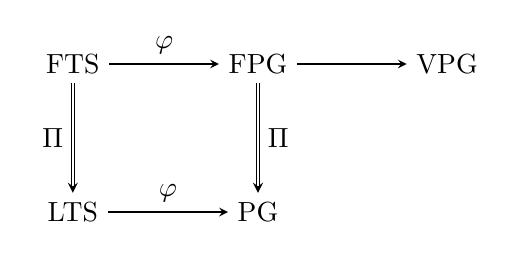
\begin{tikzpicture}
\matrix (m) [matrix of math nodes,row sep=4em,column sep=4em,minimum width=2em]
{
	\text{FTS} & \text{FPG} & \text{VPG} \\
	\text{LTS} & \text{PG} \\};
\path[-stealth]
(m-1-1) edge [double] node [left] {$\Pi$} (m-2-1)
edge node [above] {$\varphi$} (m-1-2)
(m-2-1.east|-m-2-2) edge node [above] {$\varphi$}
(m-2-2)
(m-1-2) edge [double] node [right] {$\Pi$} (m-2-2)
edge (m-1-3);
\end{tikzpicture}\\
Finally we show that solving VPGs, ie. finding the winning sets for all configurations, can be used to verify FTSs.
\begin{theorem}
	\label{the_VPG_ver_FTS}
	Given:
	\begin{itemize}
		\item FTS $M = (S, Act, trans, s_0, N, P, \gamma)$,
		\item closed modal mu-calculus formula $\varphi$,
		\item product $p \in P$ and
		\item state $s \in S$
	\end{itemize}
	it holds that $(M_{|p}, s) \models \varphi$ if and only if $(s, \varphi) \in W_0^{p}$ in $\textit{FPG2VPG}(\textit{FTS2FPG}(M, \varphi))$.
	\begin{proof}
		Let $W_0^{p}$ and $W_1^{p}$ denote the winning sets for game $\textit{FPG2VPG}(\textit{FTS2FPG}(M, \varphi))$. And $Q_0^{p}$ and $Q_1^{p}$ denote the winning sets for game $\textit{FTS2FPG}(M, \varphi)$.
		
		Using theorem \ref{the_FPG_ver_FTS} we find that $(M_{|p}, s) \models \varphi$ if and only if $(s, \varphi) \in Q_0^{p}$. If $(s, \varphi) \in Q_0^{p}$ then we find by using theorem \ref{the_FPG_sub_VPG} that $(s, \varphi) \in W_0^{p}$. If $(s, \varphi) \not\in Q_0^{p}$ then $(s, \varphi) \in Q_1^{p}$ and therefore $(s, \varphi) \in W_1^{p}$ and $(s, \varphi) \not\in W_0^{p}$.
	\end{proof}
\end{theorem}



\section{Variability parity games}
Next we will introduce \textit{variability parity games} (VPGs). VPGs are very similar to FPGs, they do however abstract from the notion of features and instead uses configuration for a syntactically more pleasant representation that is not solely tailored for FTSs. Furthermore in VPGs deadlocks are removed and therefore only having to reason about infinite paths and no longer about finite paths. Finally we will show the relation between VPGs and FTS verification, which is almost identical to the relation between FPGs and FTS verification.

First we introduce VPGs:
\begin{definition}
\label{def_VPG}
A variability parity game (VPG) is a tuple $(V,V_0, V_1, E, \rho, \mathfrak{C}, \theta)$, where:
\begin{itemize}
	\item $V = V_0 \cup V_1$ and $V_0 \cap V_1 = \emptyset$,
	\item $V_0$ is the set of vertices owned by player $0$,
	\item $V_1$ is the set of vertices owned by player $1$, 
	\item $E \subseteq V \times V$ is the edge relation; we assume that $E$ is total, i.e. for all $v\in V$ there is some $w \in V$ such that $(v,w) \in E$,
	\item $\rho :  V \rightarrow \mathbb{N}$ is a priority assignment,
	\item $\mathfrak{C}$ is a finite set of configurations,
	\item $\theta : E \rightarrow \mathcal{P}(\mathfrak{C})\ \backslash\ \{0\}$ is the configuration mapping, satisfying for all $v \in V$, $\bigcup\{\theta(v,w)|(v,w) \in E\} = \mathfrak{C}$.
\end{itemize}
\end{definition}
A VPG is played similarly to a PG, however the game is played for a specific configuration $c \in \mathfrak{C}$. Player $\alpha$ can only move the token from $v \in V_\alpha$ to $w \in V$ if $(v,w) \in E$ and $c \in \theta(v,w)$. Furthermore VPGs don't have deadlocks, therefore every play results in an infinite path.

A game played for configuration $c \in \mathfrak{C}$ results in winning sets $W_0^c$ and $W_1^c$, which are defined similar to the $W_0$ and $W_1$ winning sets for parity games.

\begin{definition}
\label{def_VPG_proj} The projection from VPG $G = (V, V_0, V_1, E, \rho, \mathfrak{C}, \theta)$ to a configuration $c \in \mathfrak{C}$, noted $G_{|c}$, is the parity game $(V, V_0, V_1, E', \rho)$ where $E' = \{ e\in E | c \in \theta(e)\}$.
\end{definition}

Playing VPG $G$ for a specific configuration $c \in \mathfrak{C}$ is the same as playing the PG $G_{|c}$. Any path that is valid in $G$ for $c$ is also valid in $G_{|c}$ and vice versa. Therefore the strategies are also interchangeable, furthermore the winning sets $W_\alpha$ for $G_{|c}$ and $W_\alpha^c$ for $G$ are identical. Since parity games are positionally determined so are VPGs. Similarly, since finite parity games are decidable, so are finite VPGs.
\subsection{Creating variability parity games}
We will define a translation from an FPG to a VPG. This relation is shown in the following diagram:
\\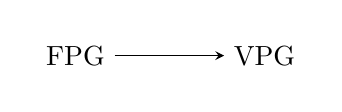
\begin{tikzpicture}
\matrix (m) [matrix of math nodes,row sep=4em,column sep=4em,minimum width=2em]
{
	\text{FPG} & \text{VPG} \\
};
\path[-stealth]
(m-1-1)
edge (m-1-2);
\end{tikzpicture}\\
To do so we have to translate products to configuration, which is trivial, furthermore we have to make the FPG deadlock free. This is done by creating two losing vertices $l_0$ and $l_1$ such that player $\alpha$ loses when the token is in vertex $l_\alpha$. Any vertex that can not move for a configuration will get an edge that is admissible for that configuration towards one of the losing vertices.
\begin{definition}
	\label{def_FPG2VPG}
	FPG2VPG($G^F$) converts FPG $G^F = (V^F, V_0^F, V_1^F, E^F, \rho^F, N, P, \gamma)$ to VPG $G = (V, V_0, V_1, E, \rho, \mathfrak{C}, \theta)$.
	
	Let $P$ be defined as  $\{p_0, p_1, \dots, p_m\}$, we define $\mathfrak{C} = \{c_0, c_1, \dots, c_m\}$.
	
	We create vertices $l_0$ and $l_1$ and define $V_0 = V_0^F \cup \{l_0\}$, $V_1 = V_1^F \cup \{l_1\}$ and $V = V_0 \cup V_1$.
	
	We construct $E$ by first making $E = E^F$ and adding edges $(l_0, l_0)$ and $(l_1, l_1)$ to $E$. Simultaneously we construct $\theta$ by first making $\theta(e) = \{c_i \in \mathfrak{C} | p_i \models \gamma(e)\}$ for every $e \in E^F$. Furthermore $\theta(l_0,l_0) = \theta(l_1,l_1) = \mathfrak{C}$.
	
	Next, for every vertex $v \in V_\alpha$ with $\alpha = \{0,1\}$, we have $C = \mathfrak{C} \backslash \bigcup \{\theta(v,w)|(v,w) \in E\}$. If $C \neq \emptyset$ then we add $(v, l_\alpha)$ to $E$ and make $\theta(v,l_\alpha) = C$.
	Finally we have 
	\[ \rho(v) = \begin{cases}
	1  & \text{if } v = l_0 \\
	0 & \text{if } v = l_1 \\
	\rho^F(v) &\text{otherwise}
	\end{cases} \]
\end{definition}
Again considering our previous working example we can translate the FPG shown in figure \ref{fig:exverfpg} to the VPG shown in figure \ref{fig:exvevpg}. Where $c_0$ corresponds to product $\emptyset$, $c_1$ corresponds to $\{f\}$ and $c_2$ to $\{f,g\}$.
\begin{figure}[h]
	\centering
	\includegraphics[scale=0.3]{Examples/ExamleVerification/VPG}
	\caption[VPG]{VPG}
	\label{fig:exvevpg}
\end{figure}

\subsection{FTS verification using VPG}
We have shown in theorem \ref{the_FPG_ver_FTS} that we can use an FPG to verify an FTS. Next we will show that a winning set in the FPG $M$ is the subset of the winning set in the VPG $FPG2VPG(M)$.
\begin{theorem}
	\label{the_FPG_sub_VPG}
	Given:
	\begin{itemize}
		\item FPG $G^F = (V^F, V_0^F, V_1^F, E^F, \rho^F, N, \{p_0, p_1, \dots, p_m\}, \gamma)$,
		\item product $p_i$
	\end{itemize}
	we have for winning sets $W_\alpha^{p_i}$ in $G$ and $W_\alpha^{c_i}$ in FPG2VPG($G^F$) that $W_\alpha^{p_i} \subseteq W_\alpha^{c_i}$ for any $\alpha \in \{0,1\}$.
	\begin{proof}
		Let $G = (V,V_0,V_1, E, \rho, \mathfrak{C},\theta) =$ FPG2VPG($G^F$). Consider finite play $\pi$ that is valid in game $G^F$ for product $p_i$. We have for every $(\pi_i, \pi_{i+1})$ in $\pi$ that $(\pi_i, \pi_{i+1}) \in E^F$ and $p_i \models \gamma((\pi_i, \pi_{i+1}))$. From the $FPG2VPG$ definition (\ref{def_FPG2VPG}) it follows that $(\pi_i, \pi_{i+1}) \in E$ and $c_i \in \theta(\pi_i, \pi_{i+1})$. So we can conclude that path $\pi$ is also valid in game $G$ for configuration $c_i$. Since the play is finite the winner is determined by the last vertex $v$ in $\pi$, player $\alpha$ wins such that $v \in V_{\overline{\alpha}}$. Furthermore we know, because the play is finite, that there exists no $(v,w) \in E^F$ with $p \models \gamma(v,w)$. From this we can conclude that $(v, l_{\overline{\alpha}}) \in E$ and $c_i \in \theta(v, l_{\overline{\alpha}})$. Vertex $l_{\overline{\alpha}}$ has one outgoing edge, namely to itself. So finite play $\pi$ will in game $G^F$ results in an infinite play $\pi(l_{\overline{\alpha}})^\omega$. Vertex $l_{\overline{\alpha}}$ has a priority with the same parity as player $\alpha$, so player $\alpha$ wins the infinite play in $G$ for configuration $c_i$.
		
		Consider infinite play $\pi$ that is valid in game $G^F$ for product $p_i$. As shown above this play is also valid in game $G$ for configuration $c_i$. Since the win conditions of both games are the same the play will result in the same winner.
		
		Consider infinite play $\pi$ that is valid in game $G$ for configuration $c_i$. We distinguish two cases:
		\begin{itemize}
			\item If $l_\alpha$ doesn't occur in $\pi$ then the path is also valid for game $G^F$ with product $p_i$ and has the same winner.
			\item If $\pi = \pi'(l_\alpha)^\omega$ with no occurrence $l_\alpha$ in $\pi'$ then the winner is player $\overline{\alpha}$. The path $\pi'$ is valid for game $G^F$ with product $p_i$. Let vertex $v$ be the last vertex of $\pi'$. Since $(v, l_\alpha) \in E$ and $c_i \in \theta(v,l_\alpha)$ we know that there is no $(v,w) \in E^F$ with $p_i \models \gamma(v,w)$ and that vertex $v$ is owned by player $\alpha$. So in game $G^F$ player $\alpha$ can't move at vertex $v$ and therefore loses the game (in which case the winner is also $\overline{\alpha}$.
		\end{itemize}
		
		We have shown that every path (finite or infinite) in game $G^F$ with product $p_i$ can be played in game $G$ with configuration $c_i$ and that they have the same winner. Furthermore every infinite path in game $G$ with configuration $c_i$ can be either played as an infinite path or the first part of the path can be played in $G^F$ with product $p_i$ and they have the same winner. From this we can conclude that the theorem holds.
	\end{proof}
\end{theorem}
We can conclude the diagram depicting the relation between the different games and transition systems:\\
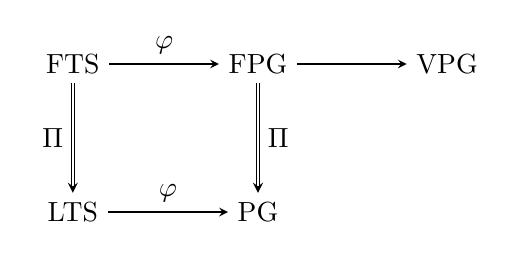
\begin{tikzpicture}
\matrix (m) [matrix of math nodes,row sep=4em,column sep=4em,minimum width=2em]
{
	\text{FTS} & \text{FPG} & \text{VPG} \\
	\text{LTS} & \text{PG} \\};
\path[-stealth]
(m-1-1) edge [double] node [left] {$\Pi$} (m-2-1)
edge node [above] {$\varphi$} (m-1-2)
(m-2-1.east|-m-2-2) edge node [above] {$\varphi$}
(m-2-2)
(m-1-2) edge [double] node [right] {$\Pi$} (m-2-2)
edge (m-1-3);
\end{tikzpicture}\\
Finally we show that VPGs can be used to verify FPGs.
\begin{theorem}
	\label{the_VPG_ver_FTS}
	Given:
	\begin{itemize}
		\item FTS $M = (S, Act, trans, s_0, N, \{p_0,\dots,p_m\}, \gamma)$,
		\item closed modal mu-calculus formula $\varphi$,
		\item product $p_i \in P$ and
		\item state $s \in S$
	\end{itemize}
	it holds that $M_{|p_i}, s \models \varphi$ if and only if $(s, \varphi) \in W_0^{c_i}$ in $FPG2VPG(FTS2FPG(M, \varphi))$.
	\begin{proof}
		Using theorem \ref{the_FPG_ver_FTS} we find that $M_{|p_i}, s \models \varphi$ if and only if $(s, \varphi) \in W_0^{p_i}$ for game $FTS2FPG(M, \varphi)$. If $(s, \varphi) \in W_0^{p_i}$ then we find by using theorem \ref{the_FPG_sub_VPG} that $(s, \varphi) \in W_0^{c_i}$ for game $FPG2VPG(FTS2FPG(M, \varphi))$. If $(s, \varphi) \not\in W_0^{p_i}$ then $(s, \varphi) \in W_1^{p_i}$ and therefore $(s, \varphi) \in W_1^{c_i}$ for game $FPG2VPG(FTS2FPG(M, \varphi))$ and $(s, \varphi) \not\in W_0^{c_i}$.
	\end{proof}
\end{theorem}
This theorem concludes the model verification technique depicted in figure \ref{fig:ftsverificationusingvpg}.
\pagebreak
\part{Solving variability parity games}
\section{Introduction}
For solving VPGs we distinguish two general approaches, the first approach is to simply project the VPG to the different configurations and solve all the resulting parity games independently. We call this \textit{independently} solving a VPG. Alternatively we solve the VPG \textit{collectively}, where a VPG is solved in its entirety and similarities between the configurations are used to improve performance. 

In the next sections we explore collective algorithms and analyse their time complexity. We aim to solve VPGs originating from model verification problems, such VPGs generally have certain properties that a completely random VPG might not have. In general parity games originating from model verification problems have a relatively low number of distinct priorities compared to the number of vertices because new priorities are only introduced when fixed points are nested in the $\mu$-calculus formula. Furthermore the transition guards of featured transition systems are expressed over features. In general these transition guards will be quite simple, specifically excluding or including a small number of features.

\subsection{Global vs local solving}
Parity games can be solved \textit{globally} or \textit{locally}; globally solving a parity game means that for every vertex in the game it is determined who the winner is. Locally solving a parity game means that for a specific vertex in the game it is determined who the winner is. For some applications of parity games, including model checking, there is a specific vertex that needs to be solved to solve the model checking problem so locally solving the parity game is sufficient for solving the original problem.

Similarly VPGs can be solved globally or locally where locally solving a VPG means determining for which configurations a certain vertex is won by player $0$ and for which configurations the vertex is won by player $1$.

Most parity game algorithms are concerned with global solving, when talking about solving a (V)PG we talk about globally solving it unless noted otherwise. For VPGs we consider a global and a local variant for every collective algorithm we are going to consider. When solving a VPG globally we might encounter significant differences in parts of the game or intermediate results between configurations that we don't encounter when solving it locally because we can terminate earlier. Therefore we hypothesize that the increase in performance between globally-collectively solving VPGs and locally-collectively solving VPGs is greater than the increase performance between globally-independently solving VPGs and locally-independently solving VPGs.

\section{Preliminary concepts}
First a few preliminary concept relevant to solving (V)PGs are introduced, specifically: existing parity game algorithms, symbolically representing sets and fixed-point theory.
\subsection{Symbolically representing sets}
A set can straightforwardly be represented by a collection containing all the elements that are in the set. We call this an \textit{explicit} representation of a set. We can also represent sets \textit{symbolically} in which case the set of elements is represented by some sort of formula. A typical way to represent a set symbolically is through a boolean formula encoded in a \textit{binary decision diagram} \cite{BDD_book,Handbook_BDD_Chapter}. For example the set $S = \{0,1,2,4,5,7 \}$ can be expressed by boolean formula:
\[ F(x_2,x_1,x_0) = (x_2 \vee \neg x_1 \vee \neg x_0) \wedge (\neg x_2 \vee \neg x_1 \vee x_0) \]
where $x_0,x_1$ and $x_2$ are boolean variables. The formula gives the following truth table:\\
\begin{center}
	\begin{tabular}{|c|c|}
		\hline 
		$\mathbf{x_2x_1x_0}$ & $\mathbf{F(x_2,x_1,x_0)}$ \\ 
		\hline 
		000 & 1 \\ 
		\hline 
		001 & 1 \\ 
		\hline 
		010 & 1 \\ 
		\hline 
		011 & 0 \\ 
		\hline 
		100 & 1 \\ 
		\hline 
		101 & 1 \\ 
		\hline 
		110 & 0 \\ 
		\hline 
		111 & 1 \\ 
		\hline 
	\end{tabular} 
\end{center}
The function $F$ defines set $S'$ in the following way: $S' = \{x_2x_1x_0\ |\ F(x_2,x_1,x_0) = 1 \}$. As we can see set $S'$ and $S$ represent the same numbers. We can perform set operations on sets represented as boolean functions by performing logical operations on the functions. For example, given boolean formula's $f$ and $g$ representing sets $V$ and $W$ the formula $f \wedge g$ represents set $V \cap W$.

Boolean functions can efficiently be represented in BDDs, for a comprehensive treatment of BDDs we refer to \cite{BDD_book,Handbook_BDD_Chapter}. We will note here that given $x$ boolean variables and two boolean functions encoded as BDDs we can perform binary operations $\vee,\wedge$ on them in $O(2^{2x})=O(m^2)$ where $m = 2^x$ is the maximum set size that can be represented by $x$ variables \cite{BDD_running_time,Handbook_BDD_Chapter}. The running time specifically depends on the size of the decision diagrams, in general if the boolean functions are simple then the size of the decision diagram is also small and operations can be performed quickly.

\subsection{Fixed-point theory} 
A fixed-point of a function is an element in the domain of that function such that the function maps to itself for that element. Fixed-point theory goes hand in hand with lattice theory which we introduce first.
\subsubsection{Lattices}
We introduce definitions for ordering and lattices taken from \cite{birkhoff1940lattice}.
\begin{definition}
	A partial order is a binary relation $x \leq y$ on set $S$ where for all $x,y,z \in S$ we have:
	\begin{itemize}
		\item $x \leq x$. (Reflexive)
		\item If $x \leq y$ and $y \leq x$, then $x=y$. (Antisymmetric)
		\item If $x \leq y$ and $y \leq z$, then $x \leq z$. (Transitive)
	\end{itemize}
\end{definition}

\begin{definition}
	A partially ordered set is a set $S$ and a partial order $\leq$ for that set, we denote a partially ordered set by $\langle S, \leq \rangle$.
\end{definition}

\begin{definition}
	Given partially ordered set $\langle P,\leq \rangle$ and subset $X \subseteq P$. An upper bound to $X$ is an element $a \in P$ such that $x \leq a$ for every $x\in X$. A least upper bound to $X$ is an upper bound $a \in P$ such every other upper bound is larger or equal to $a$.
	
	The term least upper bound is synonymous with the term supremum.
\end{definition}
\begin{definition}
	Given partially ordered set $\langle P,\leq \rangle$ and subset $X \subseteq P$. A lower bound to $X$ is an element $a \in P$ such that $a \leq x$ for every $x\in X$. A greatest lower bound to $X$ is a lower bound $a \in P$ such that every other lower bound is smaller or equal to $a$.
	
	The term greatest lower bound is synonymous with the term infimum.
\end{definition}

\begin{definition}
	A lattice is a partially ordered set where any two of its elements have a supremum and an infimum.
\end{definition}

\begin{definition}
	A complete lattice is a partially ordered set in which every subset has a supremum and an infimum.
\end{definition}

\begin{definition}
	A function $f : D \rightarrow D'$ is monotonic, also called order preserving, if for all $x \in D$ and $y \in D$ it holds that if $x \leq y$ then $f(x) \leq f(y)$.
\end{definition}
\subsubsection{Fixed-points}
Fixed-points are formally defined as follows:
\begin{definition}
	Given function $f : D \rightarrow D$ the value $x \in D$ is a fixed point for $f$ if and only if $f(x) = x$.
\end{definition}
\begin{definition}
	Given function $f : D \rightarrow D$ the value $x \in D$ is the least fixed point for $f$ if and only if $x$ is a fixed point for $f$ and every other fixed point for $f$ is greater or equal to $x$.
\end{definition}
\begin{definition}
	Given function $f : D \rightarrow D$ the value $x \in D$ is the greatest fixed point for $f$ if and only if $x$ is a fixed point for $f$ and every other fixed point for $f$ is less or equal to $x$.
\end{definition}
The Knaster-Tarski theorem states that least and greatest fixed points exist for some domain and function given that a few conditions hold.
The theorem, as written down by Tarski \cite{tarski1955}, states:
\begin{theorem}[Knaster-Tarski\cite{tarski1955}]
	\label{the_knaster_tarski}
	Let
	\begin{itemize}
		\item $\langle A, \leq \rangle$ be a complete lattice,
		\item $f$ be an increasing function on $A$ to $A$,
		\item $P$ be the set of all fixpoints of f.
	\end{itemize}
	Then the set $P$ is not empty and the system $\langle P, \leq \rangle$ is a complete lattice; in particular we have 
	\[ \sup P = \sup \{ x\ |\ f(x) \geq x \} \in P \]
	and
	\[ \inf P = \inf \{ x\ |\ f(x) \leq x \} \in P \]
\end{theorem}
\subsection{Parity game algorithms}
We inspect two existing parity game algorithms which are used in the collective VPG algorithms. First Zielonka's recursive algorithm which is well studied and generally considered to be one of the best performing parity game algorithm \cite{Oink,SolvingPGInPractice}. We also inspect the fixed-point iteration algorithm which tends to perform well for model-checking problems with a low number of distinct priorities \cite{BDDSolvingPG}.

\subsubsection{Zielonka's recursive algorithm}
First we consider Zielonka's recursive algorithm, created from the constructive proof given in \cite{ZIELONKA1998135}, which solves total PGs. Pseudo code is presented in algorithm \ref{alg_zlnk_org}. Zielonka's recursive algorithm has a worst-case time complexity of $O(e*n^d)$.
\begin{algorithm}
	\caption{$\textsc{RecursivePG}(\textit{PG } G = (V,V_0,V_1, E, \Omega))$}
	\label{alg_zlnk_org}
	\begin{algorithmic}[1]
		\State $m \gets \min\{ \Omega(v)\ |\ v \in V\}$
		\State $h \gets\max\{ \Omega(v)\ |\ v \in V\}$
		\If{$h = m$ or $V = \emptyset$}
		\If{$h$ is even or $V = \emptyset$}
		\State \Return $(V,\emptyset)$
		\Else
		\State \Return $(\emptyset, V)$
		\EndIf
		\EndIf
		\State $\alpha \gets 0$ if $h$ is even and $1$ otherwise
		\State $U \gets \{v \in V\ |\ \Omega(v) = h\}$
		\State $A \gets \alpha\textit{-Attr}(G, U)$
		\State $(W_0', W_1') \gets \textsc{RecursivePG}(G \backslash A)$
		\If{$W_{\overline{\alpha}}' =\emptyset$}
		\State $W_\alpha \gets A \cup W_\alpha'$
		\State $W_{\overline{\alpha}} \gets \emptyset$
		\Else
		\State $B \gets \overline{\alpha}\textit{-Attr}(G,W_{\overline{\alpha}}')$
		\State $(W_0'', W_1'') \gets \textsc{RecursivePG}(G \backslash B)$
		\State $W_\alpha \gets W_\alpha''$
		\State $W_{\overline{\alpha}} \gets W_{\overline{\alpha}}'' \cup B$
		\EndIf
		\State \Return $(W_0, W_1)$
	\end{algorithmic}
\end{algorithm}

The algorithm works for solving $G$ by taking the set of vertices with the highest priority and choosing player $\alpha$ such that $\alpha$ has the same parity as the highest priority. Next the algorithm finds all the vertices such that player $\alpha$ can force the play to one of these high priority vertices. Next this set of vertices is removed from the game and the resulting subgame is solved recursively. This subgame returns winning sets $W'_0$ and $W'_1$. Vertices in set $W'_{\overline{\alpha}}$ are won by player $\overline{\alpha}$ in the subgame but are also won by player $\overline{\alpha}$ in $G$. The algorithm tries to find all the vertices in $G$ such that player $\overline{\alpha}$ can force the play to a vertex in $W'_{\overline{\alpha}}$ and therefore winning the game. We now have a set of vertices that are definitely won by player $\overline{\alpha}$ in game $G$. In the rest of the game player $\alpha$ can keep the play from $W'_{\overline{\alpha}}$ so the algorithm solves the rest of the game recursively to find the complete winning sets for game $G$.

A complete explanation of the algorithm can be found in \cite{ZIELONKA1998135}, we do introduce definitions for the attractor set and for subgames. 

An attractor set is a set of vertices $A \subseteq V$ calculated for player $\alpha$ given set $U \subseteq V$ where player $\alpha$ has a strategy to force the play starting in any vertex in $A \backslash U$ to a vertex in $U$.

\begin{definition}\cite{ZIELONKA1998135}
	\label{def_attr}Given parity game $G = (V,V_0,V_1,E,\Omega)$ and a non-empty set $U \subseteq V$ we define $\alpha\textit{-Attr}(G,U)$ such that
	\[U_0 = U \]
	For $i \geq 0$:
	\begin{align*}
	U_{i+1} = U_i\cup
	&\{v \in V_\alpha\ |\ \exists v' \in V : v' \in U_i \wedge (v,v') \in E \}\\
	\cup &\{v \in V_{\overline{\alpha}}\ |\ \forall v' \in V :(v,v') \in E \implies v' \in U_i \}
	\end{align*}
	Finally:
	\[\alpha\textit{-Attr}(G,U) = \bigcup_{i \geq 0} U_i \]
\end{definition}

\begin{figure}
	\centering
	\begin{subfigure}{1\textwidth}
		\centering
		\includegraphics[scale=0.4]{Examples/Attr/Attr0}
		\caption{Set $U = U_0$}
	\end{subfigure}\\
	\begin{subfigure}{1\textwidth}
		\centering
		\includegraphics[scale=0.4]{Examples/Attr/Attr1}
		\caption{Set $U_1$}
	\end{subfigure}\\
	\begin{subfigure}{1\textwidth}
		\centering
		\includegraphics[scale=0.4]{Examples/Attr/Attr2}
		\caption{Set $U_2 = 0\textit{-Attr}(G,U)$}
	\end{subfigure}
	\caption{Game $G$ showing the attractor calculation for $0\textit{-Attr}(G,U)$}
	\label{fig:AttrCalcExample}
\end{figure}
Figure \ref{fig:AttrCalcExample} shows an example parity game in which an attractor set is calculated for player $0$. For set $U_2$ no more vertices can be attracted so we found the complete attractor set.

The algorithm also creates subgames, where a set of vertices is removed from a parity game to create a new parity game.

\begin{definition}\cite{ZIELONKA1998135}
	\label{def_org_subgame}
	Given a parity game $G = (V,V_0,V_1, E,\Omega)$ and $U \subseteq V$ we define the subgame $G \backslash U$ to be the game $(V', V_0', V_1', E', \Omega)$ with:
	\begin{itemize}
		\item $V' = V \backslash U$,
		\item $V_0' = V_0 \cap V'$,
		\item $V_1' = V_1 \cap V'$ and
		\item $E' = E \cap (V' \times V')$.
	\end{itemize}
\end{definition}

Note that a subgame is not necessarily total, however the recursive algorithm always creates subgames that are total (shown in \cite{ZIELONKA1998135}).

\subsubsection{Fixed-point iteration algorithm}
Parity games can be solved by solving an alternating fixed-point formula, as shown in \cite{WALUKIEWICZ2002311}. We will consider PG $G = (V,V_0,V_1, E, \Omega)$ with $d$ distinct priorities. We can apply \textit{priority compression} to make sure every priority in $G$ maps to a value in $\{0,\dots,d-1\}$ or $\{1, \dots, d\}$ \cite{SolvingInPractice,FPITE}. We assume without loss of generality that the priorities map to $\{0,\dots,d-1\}$ and that $d-1$ is even. 

Consider the following formula
\[ S(G = (V,V_0,V_1,E,\Omega)) = \nu Z_{d-1}. \mu Z_{d-2}. \dots . \nu Z_0. F_0(Z_{d-1},\dots,Z_0) \]
with
\[ F_0(Z_{d-1},\dots,Z_0) = \{ v \in V_0\ |\ \exists_{w\in V} (v,w) \in E \wedge Z_{\Omega(w)} \} \cup \{ v \in V_1\ |\ \forall_{w\in V} (v,w) \in E \implies Z_{\Omega(w)} \} \]
where $Z_i \subseteq V$. The formula $\nu X. f(X)$ solves the greatest fixed-point of $X$ in $f$, similarly $\mu X.f(X)$ solves the least fixed-point of $X$ in $f$.

To understand the formula we consider sub-formula $\nu Z_0. F_0(Z_{d-1},\dots,Z_0)$. This formula holds for vertices from which player $0$ can either force the play into a node with priority $i > 0$ for which $Z_i$ holds or the player can stay in vertices with priority $0$ indefinitely. The formula $\mu Z_0. F_0(Z_{d-1},\dots,Z_0)$ holds for vertices from which player $0$ can force the play into a node with priority $i > 0$, for which $Z_i$ holds in finitely many steps. By alternating fixed-points the formula allows infinitely many stays in even vertices and finitely many stays in odd vertices. For an extensive treatment we refer to \cite{WALUKIEWICZ2002311}.

We further inspect formula $S$. Given game $G$, consider the following subformula's:
\[ S^{d-1}(Z_{d-1}) = \mu Z_{d-2}.S^{d-2}(Z_{d-2})\]
\[ S^{d-2}(Z_{d-2}) = \nu Z_{d-3}.S^{d-3}(Z_{d-3})\]
\begin{center}
	\dots
\end{center}
\[ S^{0}(Z_0) = F_0(Z_{d-1},\dots,Z_0)\]
The fixed-point variables are all elements of $2^V$, therefore we have for every subformula the following type:
\[ S^i(Z_i) : 2^V \rightarrow 2^V \]
Furthermore, since $V$ is finite, the partially ordered set $\langle 2^V, \subseteq \rangle$ is a complete lattice.

Finally every subformula is $S^i(Z_i)$ is monotonic, ie. if $S^i(Z_i) \geq S^i(Z_i')$ then $Z_i \geq Z_i'$.

Fixed-point formula's can be solved by fixed-point iteration. As shown in \cite{Emerson:1986:MCP:900378} we can calculate $\mu X.f(X)$, where $f$ is monotonic in $X$ and $X \in 2^V$, by iterating $X$:
\[ \mu X.f(X) = \bigcup_{i \geq 0} X^i \]
where $X^i = f(X^{i-1})$ for $i > 0$ and $X^0 \subseteq \mu X.f(X)$. So picking the smallest value possible for $X_0$ will always correctly calculate $\mu X. f(X)$.

Similarly we can calculate fixed-point $\nu X.f(X)$ when $f$ is monotonic in $X$ by iterating $X$.
\[ \nu X.f(X) = \bigcap_{i \geq 0} X^i \]
where $X^i = f(X^{i-1})$ for $i > 0$ and $X^0 \supseteq \nu X.f(X)$. So picking the largest value possible for $X_0$ will always correctly calculate $\nu X. f(X)$.

Since every subformula is monotonic and maps from a value in $2^V$ to another value in $2^V$ we can apply fixed-point iteration to solve the subformula's, we choose initial values $\emptyset$ for least fixed-point variables and $V$ for greatest fixed-point variables.

An algorithm to perform the iteration is presented in \cite{FPITE} and shown in algorithm \ref{alg_FPITEorg}. This algorithm has a worst-case time complexity of $O(e * n ^d)$.
\begin{algorithm}
	\caption{Fixed-point iteration}
	\label{alg_FPITEorg}
	\begin{multicols}{2}
		\begin{algorithmic}[1]
			\Function{FPIter}{$G = (V, V_0, V_1, E, \Omega)$}
			\For{$i \gets d-1,\dots,0$}
			\State $\textsc{Init}(i)$
			\EndFor
			\Repeat
			\State $Z_0'\gets Z_0$
			\State $Z_0 \gets \textsc{Diamond}() \cup \textsc{Box}()$
			\State $i \gets 0$
			\While{$Z_i=Z_i' \wedge i < d-1$}
			\State $i \gets i+1$
			\State $Z_i' \gets Z_i$
			\State $Z_i \gets Z_{i-1}$
			\State $\textsc{Init}(i-1)$
			\EndWhile
			\Until{$i = d-1 \wedge Z_{d-1} = Z_{d-1}'$}
			\State \Return $(Z_{d-1},V\backslash Z_{d-1})$
			\EndFunction
		\end{algorithmic}\bigskip\bigskip
		\begin{algorithmic}[1]
			\Function{Init}{$i$}
			\State $Z_i \gets \emptyset$ if $i$ is odd, $V$ otherwise
			\EndFunction
		\end{algorithmic}\bigskip
		\begin{algorithmic}[1]
			\Function{Diamond}{}
			\State \Return $\{ v \in V_0\ |\ \exists_{w\in V} (v,w) \in E \wedge w \in Z_{\Omega(w)}\}$
			\EndFunction
		\end{algorithmic}\bigskip
		\begin{algorithmic}[1]
			\Function{Box}{}
			\State \Return $\{ v \in V_1\ |\ \forall_{w\in V} (v,w) \in E \implies w \in Z_{\Omega(w)}\}$
			\EndFunction
		\end{algorithmic}
	\end{multicols}
\end{algorithm}

\subsection{Locally solving parity games}
Parity games can be solved \textit{globally} or \textit{locally}; globally solving a parity game means that for every vertex in the game it is determined who the winner is. Locally solving a parity game means that for a specific vertex in the game it is determined who the winner is. For some applications of parity games, including model checking, there is a specific vertex that needs to be solved to solve the model checking problem so locally solving the parity game is sufficient for solving the original problem.

Most parity game algorithms are concerned with global solving, when talking about solving a PG we talk about globally solving it unless stated otherwise. 

\section{Unified parity games}
\label{sec_unified_pg}
We can consider a VPG as a PG that is the union of all its projections. We call the resulting PG the \textit{unification} of the VPG.
\begin{definition}
Given VPG $\hat{G} = (\hat{V},\hat{V}_0,\hat{V}_1, \hat{E},\hat{\Omega}, \mathfrak{C},\theta)$ we define the unification of $\hat{G}$, denoted as $\hat{G}_{\downarrow}$, as
\[  \hat{G}_{\downarrow} = \bigcup_{c\in \mathfrak{C}}\hat{G}_{|c} \]
where the union of two PGs is trivially defined as
\[ (V,V_0,V_1,E,\Omega) \cup (V',V_0',V_1',E',\Omega') = (V \uplus V', V_0 \uplus V_0', V_1 \uplus V_1', E \uplus E', \Omega \uplus \Omega') \]
\end{definition}
We will use the hat decoration ($\hat{G},\hat{V},\hat{E},\hat{\Omega},\hat{W}$) when referring to a VPG and use no hat decoration when referring to a PG.

Every vertex in game $\hat{G}_{\downarrow}$ originates from a configuration and an original vertex. Therefore we can consider every vertex in a unification as a pair consisting of a vertex and a configuration, ie. $V = \mathfrak{C} \times \hat{V}$. We can consider edges in a unification similarly, ie. $E \subseteq (\mathfrak{C} \times \hat{V}) \times (\mathfrak{C} \times \hat{V})$. Note that edges don't cross configurations, ie. for every $((c,\hat{v}) , (c',\hat{v}')) \in E$ we have $c = c'$.

If we solve the PG that is the unification of a VPG we have solved the VPG, as shown in the next theorem .
\begin{theorem}
	\label{theA_solve_UVPG_is_solve_VPG}
	Given VPG $\hat{G} =  (\hat{V},\hat{V}_0,\hat{V}_1, \hat{E},\hat{\Omega}, \mathfrak{C},\theta)$. For winning sets $W_0$ and $W_1$ for game $\hat{G}_{\downarrow}$ and winning sets $\hat{W}^c_0$ and $\hat{W}^c_1$ for some configuration $c \in \mathfrak{C}$ it holds that
	\[(c,\hat{v}) \in W_\alpha \iff \hat{v} \in \hat{W}^c_\alpha  \text{, for }\alpha \in \{0,1\}  \]
	\begin{proof}
		The bi-implication is equal to  the following to implications.
		\[ (c,\hat{v}) \in W_\alpha \implies \hat{v} \in \hat{W}^c_\alpha  \text{, for }\alpha \in \{0,1\} \]
		and
		\[ (c,\hat{v}) \notin W_\alpha\implies \hat{v} \notin \hat{W}^c_\alpha \text{, for }\alpha \in \{0,1\}  \]
		
		Since the winning sets partition the game we have $\hat{v} \notin \hat{W}^c_\alpha \implies \hat{v} \in \hat{W}^c_{\overline{\alpha}}$ (similar for set $W$). Therefore it is sufficient to prove the first implication.
		
		Let $(c,\hat{v}) \in W_\alpha$, player $\alpha$ has a strategy to win game $\hat{G}_{\downarrow}$ from vertex $(c,\hat{v})$. Since $\hat{G}_{\downarrow}$ is the union of all the projections of $\hat{G}$ we can apply the same strategy to game $\hat{G}_{|c}$ to win vertex $\hat{v}$ as player $\alpha$. Because we can win $\hat{v}$ in the projection of $\hat{G}$ to $c$ we have $\hat{v} \in \hat{W}^c_\alpha$.
	\end{proof}
\end{theorem}

One of the properties of a PG is its totality; a game is total if every vertex has at least 1 outgoing vertex. Plays in a total PG will always result in an infinite path. VPGs are total, meaning that every vertex has, for every configuration $c \in \mathfrak{C}$ at least 1 outgoing vertex admitting $c$. Because VPGs are total a unified VPG is also total. For unified VPGs we can however further investigate its totality by introducing the notion of being total for every configuration. 
\begin{definition}
	A unified VPG $(V,V_0,V_1,E,\Omega)$ is total for every configuration iff for every $(c,v) \in V$ there exists a $(c,v') \in V$ such that $((c,v),(c,v')) \in E$.
\end{definition}

It follows that if a unified VPG is total then it is also total for every configuration as shown in the following lemma.
\begin{lemma}
	\label{lem_UVPG_total}
	A unified VPG $G = (V,V_0,V_1,E,\Omega)$ that is total is also total for every configuration.
	\begin{proof}
		Since $G$ is total we have for every $(c,v) \in V$ that there exists a $(c',v') \in V$ such that $((c,v),(c',v')) \in E$. Because unified VPGs don't have edges cross configurations we find that $c = c'$ and therefore $G$ is total for every configuration.
	\end{proof}
\end{lemma}


\subsubsection{Representing unified variability parity games}
Unified VPGs have a specific structure because they are the union of parity games that have the same vertices with the same owner and priority. Because they have the same priority we don't actually need to create a new function that is the unification of all the projections, we can simply use the original priority assignment function because the following relation holds:
\[ \hat{\Omega}(c,\hat{v}) = \Omega(\hat{v}) \]
Similarly we can use the original partition sets $\hat{V}_0$ and $\hat{V}_1$ instead of having the new partition $V_0$ and $V_1$ because the following relations holds:
\[ (c,\hat{v}) \in V_0 \iff \hat{v}\in \hat{V}_0 \]
\[ (c,\hat{v}) \in V_1 \iff \hat{v}\in \hat{V}_1 \]

So instead of considering unified VPG $(V,V_0,V_1,E,\Omega)$ we will consider $(V,\hat{V}_0,\hat{V}_1,E,\hat{\Omega})$. 

Using this definition we can easily project a unified VPG back to one of the parity games.
\begin{definition}
	The projection of unified VPG $G = (V,\hat{V}_0, \hat{V}_1,E,\hat{\Omega})$ to configuration $c$, denoted as $G_{|c}$, is the parity game $(V',\hat{V}_0,\hat{V}_1,E',\hat{\Omega})$ such that $V' = \{ \hat{v}\ |\ (c,\hat{v}) \in V \}$ and $E' = E \cap (V' \times V')$.
\end{definition}

Next we consider how we represent vertices and edges in a unified VPG. A set $X \subseteq (\mathfrak{C} \times \hat{V})$ can be represented as a complete function $f : \hat{V} \rightarrow 2^\mathfrak{C}$. The set $X$ and function $f$ are equivalent, denoted by the operator $=_\lambda$, iff the following relation holds:
\[ (c,\hat{v}) \in X \iff c \in f(\hat{v}) \]
We can also represent edges as a complete function $f : \hat{E} \rightarrow 2^\mathfrak{C}$. The set $E$ and function $f$ are equivalent, denoted by the operator $=_\lambda$, iff the following relation holds:
\[ ((c,\hat{v}),(c,\hat{v}')) \in E \iff c \in f(\hat{v},\hat{v}') \]
We write $\lambda^\emptyset$ to denote the function that maps every element to $\emptyset$, clearly $\lambda^\emptyset =_\lambda \emptyset$. We call using a set of pairs to represent vertices a \textit{set-wise} representation and using functions to represent vertices a \textit{function-wise} representation.

\section{Recursive algorithm}
We can use the original Zielonka's recursive algorithm to solve VPGs, to do so we will first consider a method of creating a parity game from a VPG, called \textit{unification}.
\subsection{Unified parity games}
We can create a PG from a VPG by taking all the projections of the VPG, which are PGs, and combining them into one PG by taking the union of them. We call the resulting PG the \textit{unification} of the VPG. A parity game that is the result of a unification is called a \textit{unified PG}, also any total subgame of it will be called a unified PG. A unified PG always has a VPG from which it originated.
\begin{definition}
	Given VPG $\hat{G} = (\hat{V},\hat{V}_0,\hat{V}_1, \hat{E},\hat{\Omega}, \mathfrak{C},\theta)$ we define the unification of $\hat{G}$, denoted as $\hat{G}_{\downarrow}$, as
	\[  \hat{G}_{\downarrow} = \biguplus_{c\in \mathfrak{C}}\hat{G}_{|c} \]
	where the union of two PGs is defined as
	\[ (V,V_0,V_1,E,\Omega) \uplus (V',V_0',V_1',E',\Omega') = (V \uplus V', V_0 \uplus V_0', V_1 \uplus V_1', E \uplus E', \Omega \uplus \Omega') \]
\end{definition}
We will use the hat decoration ($\hat{G},\hat{V},\hat{E},\hat{\Omega},\hat{W}$) when referring to a VPG and use no hat decoration when referring to a PG.

Every vertex in game $\hat{G}_{\downarrow}$ originates from a configuration and an original vertex. Therefore we can consider every vertex in a unification as a pair consisting of a vertex and a configuration, ie. $V = \mathfrak{C} \times \hat{V}$. We can consider edges in a unification similarly, so $E \subseteq (\mathfrak{C} \times \hat{V}) \times (\mathfrak{C} \times \hat{V})$. Note that edges don't cross configurations so for every $((c,\hat{v}) , (c',\hat{v}')) \in E$ we have $c = c'$. Figure \ref{fig:VPG2UPG} shows an example of a unification.

\begin{figure}[h]
	\centering
	\begin{subfigure}{1\textwidth}
		\centering
		\includegraphics[scale=0.4]{Examples/UPG/VPG}
		\caption{VPG consisting of 2 configurations}
	\end{subfigure}\\
	\begin{subfigure}{1\textwidth}
		\centering
		\includegraphics[scale=0.4]{Examples/UPG/UPG}
		\caption{Unified PG, created from unifying the two projections}
	\end{subfigure}
	\caption{A VPG with its corresponding unified PG}
	\label{fig:VPG2UPG}
\end{figure}

If we solve the PG that is the unification of a VPG we have solved the VPG, as shown in the next theorem.
\begin{theorem}
	\label{theA_solve_UVPG_is_solve_VPG}
	Given 
	\begin{itemize}
		\item VPG $\hat{G} =  (\hat{V},\hat{V}_0,\hat{V}_1, \hat{E},\hat{\Omega}, \mathfrak{C},\theta)$,
		\item some configuration $c \in \mathfrak{C}$,
		\item winning sets $\hat{W}^c_0$ and $\hat{W}^c_1$ for game $\hat{G}$ and
		\item winning sets $W_0$ and $W_1$ for game $\hat{G}_{\downarrow}$
	\end{itemize}
	it holds that
	\[(c,\hat{v}) \in W_\alpha \iff \hat{v} \in \hat{W}^c_\alpha  \text{, for }\alpha \in \{0,1\}  \]
	\begin{proof}
		The bi-implication is equal to  the following to implications.
		\[ (c,\hat{v}) \in W_\alpha \implies \hat{v} \in \hat{W}^c_\alpha  \text{, for }\alpha \in \{0,1\} \]
		and
		\[ (c,\hat{v}) \notin W_\alpha\implies \hat{v} \notin \hat{W}^c_\alpha \text{, for }\alpha \in \{0,1\}  \]
		
		Since the winning sets partition the game we have $\hat{v} \notin \hat{W}^c_\alpha \implies \hat{v} \in \hat{W}^c_{\overline{\alpha}}$ (similar for set $W$). Therefore it is sufficient to prove only the first implication.
		
		Let $(c,\hat{v}) \in W_\alpha$, player $\alpha$ has a strategy to win game $\hat{G}_{\downarrow}$ from vertex $(c,\hat{v})$. Since $\hat{G}_{\downarrow}$ is the union of all the projections of $\hat{G}$ we can apply the same strategy to game $\hat{G}_{|c}$ to win vertex $\hat{v}$ as player $\alpha$. Because we can win $\hat{v}$ in the projection of $\hat{G}$ to $c$ we have $\hat{v} \in \hat{W}^c_\alpha$.
	\end{proof}
\end{theorem}

\subsubsection{Projections and totality}
A unified PG can be projected back to one of the games from which it is the union.
\begin{definition}
	The projection of unified PG $G = (V,V_0, V_1,E,{\Omega})$ to configuration $c$, denoted as $G_{|c}$, is the parity game $(V',{V}_0,{V}_1,E',{\Omega})$ such that $V' = \{ {v}\ |\ (c,{v}) \in V \}$ and $E' = \{ ({v},{w})\ |\ ((c,{v}),(c,{w})) \in E \} $.
\end{definition}

One of the properties of a PG is its totality; a game is total if every vertex has at least 1 outgoing vertex. VPGs are also total, meaning that every vertex has, for every configuration $c \in \mathfrak{C}$, at least 1 outgoing vertex admitting $c$. Because VPGs are total their unifications are also total. Since edges in a unified PG don't cross configurations we can conclude that a unified PG is total iff every projection is total.

\subsection{Solving unified PGs}
We can solve a unified PG using Zielonka's recursive algorithm. The algorithm revolves around the attractor operation. Consider the example presented in figure \ref{fig:VPG2UPG}. Vertices with the highest priority are 
\[ \{(c_1,v_0),(c_2,v_0)\}\]
attracting these for player $0$ gives the set 
\begin{align*}
\{(c_1,v_0),&(c_2,v_0),\\
(c_1,v_1),&(c_2,v_1),\\
 &(c_2,v_2)\}
\end{align*}
The algorithm tries to attract all vertices starting from $v_0$ with any configuration, in this case $v_1$ can be attracted for all configurations, $v_2$ can only be attracted for $c_2$. When edge guards are permissive, ie. they admit many configurations, then there is a good change that vertices can be attracted for multiple configurations at the same time during the algorithm. This is the idea for the collective recursive VPG algorithm we present next, we will modify the recursive algorithm to solve unified parity games such that it tries to attract multiple configurations simultaneously.

\subsection{Representing unified parity games}
In order to create an algorithm based around attracting multiple configurations we need to take a look at how unified parity games can be represented.


Unified PGs have a specific structure because they are the union of PGs that have the same vertices with the same owner and priority. Because they have the same priority we don't actually need to create a new function that is the unification of all the projections, we can simply use the original priority assignment function because the following relation holds:
\[ \Omega(c,\hat{v}) = \hat{\Omega}(\hat{v}) \]
Similarly we can use the original partition sets $\hat{V}_0$ and $\hat{V}_1$ instead of having the new partition $V_0$ and $V_1$ because the following relations holds:
\[ (c,\hat{v}) \in V_0 \iff \hat{v}\in \hat{V}_0 \]
\[ (c,\hat{v}) \in V_1 \iff \hat{v}\in \hat{V}_1 \]
So instead of considering unified PG $(V,V_0,V_1,E,\Omega)$ we will consider $(V,\hat{V}_0,\hat{V}_1,E,\hat{\Omega})$. 

Next we consider how we represent vertices and edges in a unified PG. A set $X \subseteq (\mathfrak{C} \times \hat{V})$ can be represented as a complete function $f : \hat{V} \rightarrow 2^\mathfrak{C}$. The set $X$ and function $f$ are equivalent, denoted by the operator $=_\lambda$, iff the following relation holds:
\[ (c,\hat{v}) \in X \iff c \in f(\hat{v}) \]
We can also represent edges as a complete function $f : \hat{E} \rightarrow 2^\mathfrak{C}$. The set $E$ and function $f$ are equivalent, denoted by the operator $=_\lambda$, iff the following relation holds:
\[ ((c,\hat{v}),(c,\hat{v}')) \in E \iff c \in f(\hat{v},\hat{v}') \]
We write $\lambda^\emptyset$ to denote the function that maps every element to $\emptyset$, clearly $\lambda^\emptyset =_\lambda \emptyset$. We call using a set of pairs to represent vertices and edges a \textit{set-wise} representation and using functions a \textit{function-wise} representation.

\subsection{Algorithms}
Using the recursive algorithm as a basis we can solve a VPG independently, alternatively we can solve it collectively using a set-wise presentation or a function-wise presentation. For the function-wise presentation we are working with functions mapping vertices and edges to sets of configurations. These sets of configurations can either be represented explicitly or symbolically. The following diagram shows the different algorithms:
\begin{center}
	\begin{forest}
		[Recursive algorithm, for tree={parent anchor=south, child anchor=north, align=center, s sep=5mm}
		[Independent]
		[Collective
		[Set-wise]
		[Function-wise
		[Explicit]
		[Symbolic]
		]
		]
		]
	\end{forest}
\end{center}
The independent approach uses the original algorithm, the collective set-wise approach also uses the original algorithm applied on a unified PG. The function-wise representation required modifications to the algorithm, as we try to attract multiple configurations at the same time. As we will see, this modified algorithm relies heavily on set operations over sets of configurations. As discussed in section \ref{sec:symrepconfs} sets of configurations might be particularly appropriate to represent symbolically. We hypothesize that when  this is the case and the game has a lot of commonalities then we can attract multiple configurations at the same time which can be done quickly as the symbolic set operations perform well.

\subsubsection{A note on symbolically solving games}
The function-wise algorithm has two variants: an explicit and a symbolic variant. In the explicit variant everything is represented explicitly. In the symbolic variant the sets of configurations are represented symbolically, however the graph is still represented explicitly so the algorithm is partially symbolic and partially explicit. Alternatively an algorithm could completely work symbolically by representing both the graph and the sets of configurations symbolically.

Solving parity games symbolically has been studied in \cite{BDDSolvingPG}. The obstacle is that representing graphs with a large number of nodes makes the corresponding BDDs very complex and performance decreases rapidly. As to not repeat work done in \cite{BDDSolvingPG} we only consider algorithms where we represent the graph explicitly. 

\subsection{Recursive algorithm using a function-wise representation}
We can modify the recursive algorithm to work with the function-wise representation of vertices and edges. The algorithm behaves the same, only operations are modified to work with the different representation.  Pseudo code for the modified algorithm is presented in algorithm \ref{alg_zlnk_UVPG}. Note that for this pseudo code no distinction is made whether the sets of configurations are represented explicitly or symbolically.
\begin{algorithm}
	\caption{$\textsc{RecursiveUVPG}(\textit{PG } G = (\\
		V : \hat{V} \rightarrow 2^\mathfrak{C},\\
		\hat{V}_0 \subseteq \hat{V},\\
		\hat{V}_1 \subseteq \hat{V},\\
		E : \hat{E} \rightarrow 2^\mathfrak{C},\\
		\hat{\Omega} : \hat{V}\rightarrow \mathbb{N}))$}\label{alg_zlnk_UVPG}
	\begin{algorithmic}[1]
		\State $m \gets \min\{ \hat{\Omega}(\hat{v})\ |\ V(\hat{v}) \neq \emptyset \}$
		\State $h \gets \max\{ \hat{\Omega}(\hat{v})\ |\ V(\hat{v}) \neq \emptyset \}$
		\If{$h = m$ or $V = \lambda^\emptyset$}
		\If{$h$ is even or $V = \lambda^\emptyset$}
		\State \Return $(V,\lambda^\emptyset)$
		\Else
		\State \Return $(\lambda^\emptyset, V)$
		\EndIf
		\EndIf
		\State $\alpha \gets 0$ if $h$ is even and $1$ otherwise
		\State $U \gets \lambda^\emptyset$, $U(\hat{v}) \gets V(\hat{v})$ for all $\hat{v}$ with $\hat{\Omega}(\hat{v}) = h$
		\State $A \gets \alpha\textit{-FAttr}(G, U)$
		\State $(W_0', W_1') \gets \textsc{RecursiveUVPG}(G \backslash A)$
		\If{$W_{\overline{\alpha}}' =\lambda^\emptyset$}
		\State $W_\alpha \gets A \cup W_\alpha'$
		\State $W_{\overline{\alpha}} \gets \lambda^\emptyset$
		\Else
		\State $B \gets \overline{\alpha}\textit{-FAttr}(G,W_{\overline{\alpha}}')$
		\State $(W_0'', W_1'') \gets \textsc{RecursiveUVPG}(G \backslash B)$
		\State $W_\alpha \gets W_\alpha''$
		\State $W_{\overline{\alpha}} \gets W_{\overline{\alpha}}'' \cup B$
		\EndIf
		\State \Return $(W_0, W_1)$
	\end{algorithmic}
\end{algorithm}

We introduce a modified attractor definition to work with the function-wise representation.
\begin{definition}
		\label{def_Uattr}Given unified PG $G = (V, \hat{V}_0,\hat{V}_1,E,\hat{\Omega})$ and a non-empty set $U \subseteq V$, both represented function-wise, we define $\alpha\textit{-FAttr}(G,U)$ such that
	\[U_0 = U \]
	For $i \geq 0$:
	\[
	U_{i+1}(\hat{v}) = U_i(\hat{v}) \cup \begin{cases}
V(\hat{v}) \cap \bigcup_{\hat{v}'} (E(\hat{v},\hat{v}') \cap U_i(\hat{v}')) & \text{if } \hat{v} \in \hat{V_{\alpha}}\\
V(\hat{v}) \cap \bigcap_{\hat{v'}}((\mathfrak{C} \backslash E(\hat{v},\hat{v}')) \cup U_i(\hat{v}') & \text{if }\hat{v} \in  \hat{V_{\overline{\alpha}}} \\
	\end{cases}
	\]
	Finally:
	\[\alpha\textit{-FAttr}(G,U) = \bigcup_{i \geq 0} U_i \]
\end{definition}
We will now prove that the function-wise attractor definition gives a result equal to the original definition.
\begin{lemma}
	\label{lem_attr_equal}
	Given unified PG $G = (\mathcal{V},\hat{V}_0,\hat{V}_1, \mathcal{E}, \hat{\Omega})$ and set $\mathcal{U} \subseteq \mathcal{V}$ the function-wise attractor $\alpha\textit{-FAttr}(G,\mathcal{U})$ is equivalent to the set-wise attractor $\alpha\textit{-Attr}(G,\mathcal{U})$ for any $\alpha \in \{0,1\}$.
	\begin{proof}
		Let $V,E,U$ be the set-wise representation and $V^\lambda,E^\lambda,U^\lambda$ be the function-wise representation of $\mathcal{V},\mathcal{E},\mathcal{U}$ respectively.
		
		The following properties hold by definition:
		\[ (c,\hat{v}) \in V \iff c \in V^\lambda(\hat{v})\]
		\[ (c,\hat{v}) \in U \iff c \in U^\lambda(\hat{v})\]
		\[ ((c,\hat{v}),(c,\hat{v}')) \in E \iff c \in E^\lambda(\hat{v},\hat{v}') \]
		
		Since the attractors are inductively defined and $U_0 =_\lambda U^\lambda_0$ (because $U =_\lambda U^\lambda$) we have to prove that for some $i \geq 0$, with $U_i =_\lambda U^\lambda_i$,  we have $U_{i+1} =_\lambda U^\lambda_{i+1}$, which holds iff:
		\[ (c,\hat{v}) \in U_{i+1} \iff c \in U^\lambda_{i+1}(\hat{v}) \]
		Let $(c,\hat{v}) \in V$ (and therefore $c \in V^\lambda(\hat{v})$), we consider 4 cases.
		\begin{itemize}
			\item Case: $\hat{v} \in \hat{V}_{\alpha}$ and $(c,\hat{v}) \in U_{i+1}$:\\
			To prove: $c \in U^\lambda_{i+1}(\hat{v})$.
			
			If $(c,\hat{v}) \in U_i$ then $c \in U^\lambda_i(\hat{v})$ and therefore $c \in U^\lambda_{i+1}(\hat{v})$. If $(c,\hat{v}) \notin U_i$ then we have $c \notin U^\lambda_i(\hat{v})$.
			
			
			Because $\hat{v} \in \hat{V}_{\alpha}$ and $c \in V^\lambda(\hat{v})$ we get
			\[ U^\lambda_{i+1} =\bigcup_{\hat{v}'} (E^\lambda(\hat{v},\hat{v}') \cap U^\lambda_i(\hat{v}')) \]
			
			There exists an $(c',\hat{v}') \in V$ such that $(c',\hat{v}') \in U_i$ and $((c,\hat{v}),(c',\hat{v}')) \in E$. Because edges don't cross configurations we can conclude that $c' = c$. Due to equivalence we have $c \in U^\lambda_i(\hat{v}')$ and $c \in E^\lambda(\hat{v},\hat{v}')$. If we fill this in in the above formula we can conclude that $c \in U^\lambda_{i+1}(\hat{v})$.
			\item Case: $\hat{v} \in \hat{V}_{\alpha}$ and $(c,\hat{v}) \notin U_{i+1}$:\\
			To prove: $c \notin U^\lambda_{i+1}(\hat{v})$.
			
			
			First we observe that since $(c, \hat{v}) \notin U_{i+1}$ we get $(c, \hat{v}) \notin U_{i}$ and therefore $c \notin U^\lambda_i(\hat{v})$.
			
			Because $\hat{v} \in \hat{V}_{\alpha}$ and $c \in V^\lambda(\hat{v})$ we get
\[ U^\lambda_{i+1} =\bigcup_{\hat{v}'} (E^\lambda(\hat{v},\hat{v}') \cap U^\lambda_i(\hat{v}')) \]
			
			Assume $c \in U^\lambda_{i+1}(\hat{v})$. There must exist a $\hat{v}'$ such that $c \in E^\lambda(\hat{v},\hat{v}')$ and $c \in U^\lambda_i(\hat{v}')$. Due to equivalence we have a vertex $((c,\hat{v}),(c,\hat{v}')) \in E$ and $(c,\hat{v}') \in U_i$. In which case $(c,\hat{v})$ would be attracted and would be in $U_{i+1}$ which is a contradiction.
			\item Case: $\hat{v} \in \hat{V}_{\overline{\alpha}}$ and $(c,\hat{v}) \in U_{i+1}$:\\
			To prove: $c \in U^\lambda_{i+1}(\hat{v})$.
			
			If $(c,\hat{v}) \in U_i$ then $c \in U^\lambda_i(\hat{v})$ and therefore $c \in U^\lambda_{i+1}(\hat{v})$. If $(c,\hat{v}) \notin U_i$ then we have $c \notin U^\lambda_i(\hat{v})$.
			
			Because $\hat{v} \in \hat{V}_{\overline{\alpha}}$ we get
			\[ U^\lambda_{i+1} =V^\lambda(\hat{v}) \cap \bigcap_{\hat{v'}}((\mathfrak{C} \backslash E^\lambda(\hat{v},\hat{v}')) \cup U^\lambda_i(\hat{v}') \]
			
			Assume $c \notin U^\lambda_{i+1}(\hat{v})$. Because $c \in V^\lambda(\hat{v})$ there must exist an $\hat{v}$ such that
			\[ c \notin ((\mathfrak{C} \backslash E^\lambda(\hat{v},\hat{v}')) \text{ and } c \notin U^\lambda_i(\hat{v}') \]
			which is equal to
			\[ c \in E^\lambda(\hat{v},\hat{v}') \text{ and } c \notin U^\lambda_i(\hat{v}') \]
			By equivalence we have $((c,\hat{v}),(c,\hat{v}')) \in E$ and $(c,\hat{v}') \notin U_i$. Which means that $(c,\hat{v})$ will not be attracted and $(c,\hat{v}) \notin U_{i+1}$ which is a contradiction.
			\item Case: $\hat{v} \in \hat{V}_{\overline{\alpha}}$ and $(c,\hat{v}) \notin U_{i+1}$:\\
			To prove: $c \notin U^\lambda_{i+1}(\hat{v})$.
			
			First we observe that since $(c, \hat{v}) \notin U_{i+1}$ we get $(c, \hat{v}) \notin U_{i}$ and therefore $c \notin U^\lambda_i(\hat{v})$.
			
			Because $\hat{v} \in \hat{V}_{\overline{\alpha}}$ we get
			\[ U^\lambda_{i+1} =V^\lambda(\hat{v}) \cap \bigcap_{\hat{v'}}((\mathfrak{C} \backslash E^\lambda(\hat{v},\hat{v}')) \cup U^\lambda_i(\hat{v}') \]
			
			Since $(c,\hat{v})$ is not attracted there must exist a $(c,\hat{v}') \in V$ such that 
			\[ ((c,\hat{v}),(c,\hat{v}')) \in E  \text{ and } (c,\hat{v}') \notin U_i \]
			By equivalence we have 
			\[ c \in E^\lambda(\hat{v},\hat{v}')  \text{ and } c \notin U^\lambda_i(\hat{v}') \]
			Which is equal to
			\[ c \notin (\mathfrak{C} \backslash E^\lambda(\hat{v},\hat{v}'))  \text{ and } c \notin U^\lambda_i(\hat{v}') \]
			From which we conclude
			\[ c \notin ((\mathfrak{C} \backslash E^\lambda(\hat{v},\hat{v}')) \cup U^\lambda_i(\hat{v}'))) \]
			Therefore we have $c \notin U^\lambda_{i+1}(\hat{v})$.
		\end{itemize}
	\end{proof}
\end{lemma}

We also introduce a modified subgame definition to work with the function-wise representation.
\begin{definition}
	\label{def_Usubgame}
	For unified PG $G = (V,\hat{V}_0,\hat{V}_1,E,\hat{\Omega})$, represented function-wise, and set $X \subseteq V$ we define the subgame $G \backslash X = (V',\hat{V}_0,\hat{V}_1,E',\hat{\Omega})$ such that:
	\begin{itemize}
		\item $V'(\hat{v}) = V(\hat{v}) \backslash X(\hat{v})$
		\item $E'(\hat{v},\hat{v}') = E(\hat{v},\hat{v}') \cap V'(\hat{v}) \cap V'(\hat{v}')$
	\end{itemize}
\end{definition}
We prove that this new subgame definition gives a result equal to the original subgame definition. Note that when using the original subgame definition for unified PGs we can omit the modification to the partition because, as we have seen, we can use the partitioning from the VPG in the representation of unified PGs.
\begin{lemma}
	\label{lem_subgame_eq}
	Given unified PG $G = (\mathcal{V},\hat{V}_0,\hat{V}_1, \mathcal{E}, \hat{\Omega})$ and set $\mathcal{U} \subseteq \mathcal{V}$ the subgame $G \backslash \mathcal{U} = (\mathcal{V}',\hat{V}_0,\hat{V}_1,\mathcal{E}',\hat{\Omega})$ represented set-wise is equal to the subgame represented function-wise.
	\begin{proof}
		Let $V,V',E,E',U$ be the set-wise and $V^\lambda,{V^\lambda}', E^\lambda, {E^\lambda}', U^\lambda$ the function-wise representations of $\mathcal{V},\mathcal{V}', \mathcal{E}, \mathcal{E}', \mathcal{U}$ respectively. We know $V =_\lambda V^\lambda$, $E =_\lambda E^\lambda$ and $U =_\lambda U^\lambda$. To prove: $V' =_\lambda {V^\lambda}'$ and $E' =_\lambda {E^\lambda}'$.
		
		Let $(c,\hat{v}) \in V$.
		
		If $(c,\hat{v}) \in U$ then $c \in U^\lambda(\hat{v})$, also $(c,\hat{v}) \notin V'$ (by definition \ref{def_org_subgame}) and $c \notin {V^\lambda}'(\hat{v})$ (by definition \ref{def_Usubgame}).
		
		If $(c,\hat{v}) \notin U$ then $c \notin U^\lambda(\hat{v})$, also $(c,\hat{v}) \in V'$ (by definition \ref{def_org_subgame}) and $c \in {V^\lambda}'(\hat{v})$ (by definition \ref{def_Usubgame}).
		
		Let $((c,\hat{v}),(c,\hat{w})) \in E$.
		
		If $(c,\hat{v}) \in U$ then $(c,\hat{v}) \notin V'$ and $c \notin {V^\lambda}'(\hat{v})$ (as shown above). We get $((c,\hat{v}),(c,\hat{w})) \notin V' \times V'$ so $((c,\hat{v}),(c,\hat{w})) \notin E'$ (by definition \ref{def_org_subgame}). Also $c \notin {E^\lambda}'(\hat{v},\hat{w})$ (by definition \ref{def_Usubgame}).
		
		If $(c,\hat{w}) \in U$ then we apply the same logic.
		
		If neither is in $U$ then both are in $V'$ and in $V' \times V'$ and therefore the $((c,\hat{v}),(c,\hat{w})) \in E'$. Also we get $c \in {V^\lambda}'(\hat{v})$ and $c \in {V^\lambda}'(\hat{w})$ so we get $c \in {E^\lambda}'(\hat{v},\hat{w})$ (by definition \ref{def_Usubgame}).
	\end{proof}
\end{lemma}

Next we prove the correctness of the algorithm by showing that the winning sets of the function-wise algorithm are equal to the winning sets of the set-wise algorithm.
\begin{theorem}
	Given unified PG $\mathcal{G} = (\mathcal{V},\hat{V}_0,\hat{V}_1, \mathcal{E}, \hat{\Omega})$ the winning sets resulting from \textsc{RecursiveUVPG($\mathcal{G}$)} ran over the function-wise representation of $\mathcal{G}$ is equal to the winning sets resulting from \textsc{RecursivePG($\mathcal{G}$)} ran over the set-wise representation of $\mathcal{G}$.
	\begin{proof}
		Let $G = (V,\hat{V}_0,\hat{V}_1,E,\hat{\Omega})$ be the set-wise representation of $\mathcal{G}$ and $G^\lambda = (V^\lambda, \hat{V}_0, \hat{V}_1, E^\lambda, \hat{\Omega})$ be the function-wise representation of $\mathcal{G}$.
		
		Proof by induction on $\mathcal{G}$.
		
		\textbf{Base} When there are no vertices or only one priority \textsc{RecursiveUVPG($G^\lambda$)} returns $\lambda^\emptyset$ and \textsc{RecursivePG($G$)} returns $\emptyset$, these two results are equal therefore the theorem holds in this case.
		
		\textbf{Step}
		Player $\alpha$ gets the same value in both algorithms since the highest priority is equal for both algorithms.
		
		Let $U = \{(c,\hat{v}) \in V\ |\ \hat{\Omega}(\hat{v}) = h \}$ (as calculated by \textsc{RecursivePG}) and $U^\lambda(\hat{v}) = V^\lambda(\hat{v})$ for all $\hat{v}$ with $\hat{\Omega}(\hat{v}) = h$ (as calculated by \textsc{RecursiveUVPG}). We will show that $U =_\lambda U^\lambda$.
		
		Let $(c,\hat{v}) \in U$ then $\hat{\Omega}(\hat{v}) = h$, therefore $U^\lambda(\hat{v}) = V^\lambda(\hat{v})$. Since $U \subseteq V$ we have $(c,\hat{v}) \in V$ and because the equality between $V$ and $V^\lambda$ we get $c \in V^\lambda(\hat{v})$ and $c \in U^\lambda(\hat{V})$.
		
		Let $c \in U^\lambda(\hat{v})$, since $U^\lambda(\hat{v})$ is not empty we have $\hat{\Omega}(\hat{v}) = h$, furthermore $c \in V^\lambda(\hat{v})$ and therefore $(c,\hat{v}) \in V$. We can conclude that $(c, \hat{v}) \in U$ and $U =_\lambda U^\lambda$.
		
		For the rest of the algorithm it is sufficient to see that attractor sets are equal if the game and input set are equal (as shown in lemma \ref{lem_attr_equal}) and that the created subgames are equal (as shown in lemma \ref{lem_subgame_eq}). Since the subgames are equal we can apply the theorem on it by induction and conclude that the winning sets are also equal.
	\end{proof}
\end{theorem}

Theorem \ref{theA_solve_UVPG_is_solve_VPG} shows that solving a unified PG solves the VPG, furthermore the algorithm \textsc{RecursiveUVPG} correctly solves a unified PG therefore we can conclude that for VPG $\hat{G}$ vertex $\hat{v}$ is won by player $\alpha$ for configuration $c$ iff $c \in W_\alpha(\hat{v})$ with $(W_0,W_1) = \textsc{RecursiveUVPG}(G_{\downarrow})$.

\subsubsection{Function-wise attractor set}
Next we present an algorithm to calculate the function-wise attractor, the pseudo code is presented in algorithm \ref{alg_fattr_alg}. The algorithm considers vertices that are in the attracted set for some configuration, for every such vertex the algorithm tries to attract vertices that are connected by an incoming edge. If a vertex is attracted for some configuration then the incoming edges of that vertex will also be considered. We prove the correctness of the algorithm in the following lemma and theorem.
\begin{algorithm}
	\caption{$\textsc{$\alpha$-FAttractor}(G, A : \hat{V} \rightarrow 2^\mathfrak{C})$}\label{alg_fattr_alg}
	\begin{algorithmic}[1]
		\State Queue $Q \gets \{\hat{v} \in \hat{V} \ |\ A(\hat{v}) \neq \emptyset  \}$
		\While{$Q$ is not empty}
		\State $\hat{v}' \gets Q.pop()$
		\For{$E(\hat{v},\hat{v}') \neq \emptyset$}
			\If{$\hat{v} \in \hat{V}_\alpha$}
				\State $a \gets V(\hat{v}) \cap E(\hat{v},\hat{v}') \cap A(\hat{v}')$
			\Else
				\State $a \gets V(\hat{v})$
				\For{$E(\hat{v},\hat{v}'') \neq \emptyset$}
					\State $a \gets a \cap (\mathfrak{C}\backslash E(\hat{v},\hat{v}'') \cup A(\hat{v}''))$
				\EndFor
			\EndIf
			\If{$a \backslash A(\hat{v}) \neq \emptyset$}
				\State $A(\hat{v}) \gets A(\hat{v}) \cup a$
				\State $Q.push(\hat{v})$
			\EndIf
		\EndFor
		\EndWhile
		\State \Return $A$
	\end{algorithmic}
\end{algorithm}
\begin{lemma}
\label{lem_attr_requires_E}
Vertex $\hat{v}$ and configuration $c$, with $c \in V(\hat{v})$, can only be attracted if there is a vertex $\hat{v}'$ such that $c \in E(\hat{v}, \hat{v}')$ and $c \in U_i(\hat{v}')$.
	\begin{proof}
		We first observe that if $\hat{v} \in \hat{V}_\alpha$ then this property follows immediately from definition the function-wise attractor definition (\ref{def_Uattr}). If $\hat{v} \in \hat{V}_{\overline{\alpha}}$ we note that unified PGs are total and therefore all of their projections are also total. So vertex $\hat{v}$ has at least one outgoing edge for $c$, we have $\hat{w}$ such that $c \in E(\hat{v},\hat{w})$. For $\hat{v}$ with $c$ to be attracted we must have $c \in U_i(\hat{w})$.
	\end{proof}
\end{lemma}
\begin{theorem}
Set $A$ calculated by $\textsc{$\alpha$-FAttractor}(G,U)$ satisfies $A = \alpha\textit{-FAttr}(G,U)$.
	\begin{proof} We will prove two loop invariants over the while loop of the algorithm.
		
		\textbf{IV1}: For every $\hat{w} \in \hat{V}$ and $c \in \mathfrak{C}$ with $c \in A(\hat{w})$ we have $c \in \alpha\textit{-FAttr}(G,U)(\hat{w})$.
		
		\textbf{IV2}: For every $\hat{w} \in \hat{V}$ and $c \in \mathfrak{C}$ that can be attracted to $A$ either $c \in A(\hat{w})$ or there exists a $\hat{w}' \in Q$ such that $c \in E(\hat{w},\hat{w}')$.
		
		\textbf{Base}: Before the loop starts we have $A = U$, therefore IV1 holds. Furthermore all the vertices that are in $A$ for some $c$ are also in $Q$ so IV2 holds.
		
		\textbf{Step}: Consider the beginning of an iteration and assume IV1 and IV2 hold. To prove: IV1 and IV2 hold at the end of the iteration.
		
		Set $A$ only contains vertices with configurations that are in $\alpha\textit{-FAttr}(G,U)$. The set is only updated through lines 5-12 and 14 of the algorithm which reflects the exact definition of the attractor set therefore IV1 holds at the end of the iteration.
		
		Consider $\hat{w} \in \hat{V}$ and $c \in \mathfrak{C}$, we distinguish three cases to prove IV2:
		\begin{itemize}
			\item $\hat{w}$ with $c$ can be attracted by the beginning of the iteration but not by the end.
			
			This case can't happen because $A(\hat{w})$ only increases during the algorithm and the values for $E$ and $V$ are not changed throughout the algorithm.
			\item $\hat{w}$ with $c$ can't be attracted by the beginning of the iteration but can by the end.
			
			For $\hat{w}$ with $c$ to be able to be attracted at the end of the iteration there must be some $\hat{w}'$ with $c$ such that during the iteration $c$ was added to $A(\hat{w}')$ (lemma \ref{lem_attr_requires_E}). Every $\hat{w}'$ for which $A(\hat{w}')$ is updated is added to the queue (lines 13-16). Therefore we have $\hat{w}' \in Q$ with $c \in E(\hat{w},\hat{w}')$ and IV1 holds.
			\item $\hat{w}$ with $c$ can be attracted by the beginning of the iteration and also by the end.
			
			Since IV2 holds at the beginning of the iteration we have either $c \in A(\hat{w})$ or we have some $\hat{w}' \in Q$ such that $c \in E(\hat{w},\hat{w}')$. In the former case IV2 holds trivially by the end of the iteration since $A(\hat{w})$ can only increase. For the latter case we distinguish two scenario's. 
			
			First we consider the scenario where vertex $\hat{v}'$ that is considered during the iteration (line 3 of the algorithm) is $\hat{w}'$. There is a vertex $c \in E(\hat{w},\hat{w}')$ by IV2. Therefore we can conclude that $\hat{w}$ is considered in the for loop starting at line $4$ and will be attracted in lines 5-12 and added to $A(\hat{w})$ in line 14. Therefore IV2 holds by the end of the iteration.
			
			Next we consider the scenario where $\hat{v}' \neq \hat{w}'$. In this case by the end of the iteration $\hat{w}'$ will still be in $Q$ and IV2 holds.
		\end{itemize}
	
	Vertices are only added to the queue when something is added to $A$ (if statement on line 13). This can only finitely often happen because $A(\hat{v})$ can never be larger than $V(\hat{v})$ so we can conclude that the while loop terminates after a finite number of iterations.
	
		When the while loop terminates IV1 and IV2 hold so for every $\hat{w} \in \hat{V}$ and $c \in \mathfrak{C}$ that can be attracted to $A$ we have $c \in A(\hat{w})$. Since we start with $A = U$ we can conclude the soundness of the algorithm. IV1 shows the completeness.
	\end{proof}
\end{theorem}


\subsection{Running time}
We will consider the running time for solving VPG $G = (V,V_0,V_1,E,\Omega,\mathfrak{C},\theta)$ independently and collectively using the different types of representations. We will use $n$ to denote the number of vertices, $e$ the number of edges, $c$ the number of configurations and $d$ the number of distinct priorities.

The original algorithm runs in $O(e * n^d)$, if we run $c$ parity games independently we get $O(c * e * n ^d)$. We can also apply the original algorithm to a unified PG (represented set-wise) for a collective approach, in this case we get a parity game with $c*n$ vertices and $c*e$ edges. which gives a running time $O(c*e*(c*n)^d)$. However this running time can be improved by using the property that a unified PG consists of $c$ disconnected graphs as we shown next.

We have introduced three types of collective algorithms: set-wise, function-wise with explicit configuration sets and function-wise with symbolic configuration sets. In all three algorithms the running time of the attractor set is dominant, so we need three things: analyse the running time of the base cases, analyse the running time of the attractor set and analyse the recursion.

\textit{Base cases.} In the base cases the algorithm needs to do two things: find the highest and lowest priority and check if there are no more vertices in the game. For the set-wise variant we find the highest and lowest priorities by iterating all vertices, which takes $O(c*n)$. Checking if there are no more vertices is done in $O(1)$. For the function wise algorithms we can find the highest and lowest priority in $O(n)$ and checking if there are no vertices is also done in $O(n)$ since we have to check $V(\hat{v}) = \emptyset$ for every $\hat{v}$. Note that in a symbolic representation using BDDs we can check if a set is empty in $O(1)$ because the decision diagram contains a single node.

\textit{Attractor sets.} For the set-wise collective approach we can use the attractor calculation from the original algorithm which has a time complexity of $O(e)$, so for a unified PG having $c*e$ edges we have $O(c*e)$.

The function-wise variants use a different attractor algorithm. First we consider the variant where sets of configurations are represented explicitly.

Consider algorithm \ref{alg_fattr_alg}. A vertex will be added to the queue when this vertex is attracted for some configuration, this can only happen $c*n$ times, once for every vertex configuration combination. 

The first for loop considers all the incoming edges of a vertex. When we consider all vertices the for loop will have considered all edges, since we consider every vertex at most $c$ times the for loop will run at most $c*e$ times in total.

The second for loop considers all outgoing edges of a vertex. The vertices that are considered are the vertices that have an edge going to the vertex being considered by the while loop. Since the while loop considers $c*n$ vertices the second for loop runs in total at most $c * n * e$ times. The loop itself performs set operations on the set of configurations which can be done in $O(c)$. This gives a total time complexity for the attractor set of $O(n*c^2*e)$.

For the symbolic representation set operations can be done in $O(c^2)$ so we get a time complexity of $O(n*c^3*e)$.

This gives the following time complexities\\
\begin{center}
	\begin{tabular}{|c|c|c|}
		\hline 
		& Base & Attractor set \\ 
		\hline 
		Set-wise & $O(c*n)$ & $O(c*e)$  \\ 
		\hline 
		Function-wise explicit & $O(n)$ &  $O(n*c^2*e)$ \\ 
		\hline 
		Function-wise symbolic & $O(n)$ &  $O(n* c^3*e)$ \\ 
		\hline 
	\end{tabular} 
\end{center}

\textit{Recursion}. The three algorithms behave the same way with regards to their recursion, so we analyse the running time of the set-wise variant and can derive the time complexity of the others using the result.

The algorithm has two recursions, the first recursion lowers the number of distinct priorities by 1. The second recursion removes at least one edge, however the game is comprised of disjoint projections. We can use this fact use in the analyses. Consider unified PG $G$ and $A$ as specified by the algorithm. Now consider the projection of $G$ to an arbitrary configuration $q$, $G_{|q}$. If $(G\backslash A)_{|q}$ contains a vertex that is won by player $\overline{\alpha}$ then this vertex is removed in the second recursion step. If there is no vertex won by player $\overline{\alpha}$ then the game is won in its entirety and the only vertices won by player $\overline{\alpha}$ are in different projections. We can conclude that for every configuration $q$ the second recursion either removes a vertex or $(G\backslash A)_{|q}$ is entirely won by player $\alpha$. Let $\overline{n}$ denote be the maximum number of vertices that are won by player $\overline{\alpha}$ in game $(G\backslash A)_{|q}$. Since every projection has at most $n$ vertices the value for $\overline{n}$ can be at most $n$. Furthermore since $\overline{n}$ depends on $A$, which depends on the maximum priority, the value $\overline{n}$ gets reset when the top priority is removed in the first recursion. We can now write down the recursion of the algorithm:
\[ T(d,\overline{n}) \leq T(d-1,n) + T(d, \overline{n} - 1) + O(c*e) \]
When $\overline{n} = 0$ we will get $W_{\overline{\alpha}} = \emptyset$ as a result of the first recursion. In such a case there will be only 1 recursion.
\[ T(d,0) \leq T(d-1,n) + O(c*e) \]
Finally we have the base case where there is 1 priority:
\[ T(1, \overline{n}) \leq O(c*n) \]
Expanding the second recursion gives
\begin{align*}
T(d) &\leq (n+1)T(d-1) + (n+1)O(c*e)\\
T(1) &\leq O(c*n)
\end{align*}
We will now prove that $T(d) \leq (n+d)^dO(c*e)$ by induction on $d$.

\textbf{Base} $d=1$: $T(1) \leq O(c*n) \leq O(c*e) \leq (n+1)^1O(c*e)$

\textbf{Step} $d > 1$:
\begin{align*}
T(d) &\leq (n+1)T(d-1) + (n+1)O(c*e)\\
&\leq (n+1)(n+d-1)^{d-1}O(c*e) + (n+1)O(c*e)
\end{align*}
Since $n+1 \leq n+d-1$ we get:
\begin{align*}
T(d) &\leq (n+d-1)(n+d-1)^{d-1}O(c*e) + (n+1)O(c*e)\\
&\leq (n+d-1)^dO(c*e) + (n+1)O(c*e)\\
&\leq ((n+d-1)^d + n + 1)O(c*e)
\end{align*}
Using lemma \ref{lem_md_ineq} we get
\begin{align*}
T(d) &\leq (n+d)^dO(c*e)
\end{align*}
This gives a time complexity of $O(c*e*(n+d)^d) = O(c*e*n^d)$. Note that the base time complexity is subsumed in the recursion by the time complexity of the attractor set. Since the time complexity of the attractor set is higher that the time complexity of the base cases for all three variants of algorithms we can simply fill in the attractor time complexity to get $O(n*c^2*e*n^d)$ for the function-wise explicit algorithm and $O(n*c^3*e*n^d)$ for the function-wise symbolic algorithm.

The different algorithms, including their time complexities, are repeated in the diagram below:\\
\begin{center}
	\begin{forest}
	[Recursive algorithm, for tree={parent anchor=south, child anchor=north, align=center, s sep=5mm}
		[Independent\\$O(c*e*n^d)$ ]
		[Collective
			[Set-wise\\$O(c*e*n^d)$ ]
			[Function-wise
				[Explicit\\$O(n * c^2 * e * n^d)$ ]
				[Symbolic\\$O(n * c^3 * e * n^d)$ ]
			]
		]
	]
	\end{forest}
\end{center}

\subsubsection{Running time in practice}
Earlier we hypothesized that the symbolic function-wise algorithm could have the best performance of the 4 algorithms, however it has the worse case running time complexity. Our hypothesis was based on the notion that VPGs most likely have a lot of commonalities and that sets of configurations in the VPG can be represented efficiently symbolically. Next we argue why the worse case running time complexity might not represent the running time in practice.

We dissect the running time of the function-wise algorithms. The running time complexities of the collective algorithms consist of two parts: the time complexity of the attractor set times $n^d$. The function-wise attractor set time complexity also consists of two parts: the maximum number of vertices in the queue ($c*n$) times the time complexity for set operations ($O(c)$ for the explicit variant, $O(c^2)$ for the symbolic variant).

The number of vertices in the queue during attracting is at most $c*n$, however this number will only be large if we attract a very small number of configurations per time we evaluate an edge. As argued earlier we can most likely attract multiple configurations at the same time. This will decrease the number of vertices in the queue.

The time complexity of set operations is $O(c)$ when using an explicit representation and $O(c^2)$ when using a symbolic one. However, as shown in \cite{BDD_running_time}, a breadth-depth first implementation of BDDs keeps a table of already computed results. This allows us to get already calculated results in sublinear time. In total there are $2^c$ possible sets and therefore $2^{2c}$ possible set combinations and $O(2^c)$ possible set operations that can be computed. However when solving a VPG originating from an FTS there will most likely be a relatively small number of different edge guards, in which case the number of unique sets considered in the algorithm will be small and we can often retrieve a set calculation from the computed table.

We can see that even though the running time of the collective symbolic algorithm is the worse, its practical running time might be good when we are able to attract multiple configurations at the same time and have a small number of different edge guards.

\section{Pessimistic parity games}
Given a VPG with configurations $\mathfrak{C}$ we can try to determine sets $P_0,P_1$ such that the vertices in set $P_\alpha$ are won by player $\alpha \in \{0,1\}$ for any configuration in $\mathfrak{C}$. We can do so by creating a \textit{pessimistic} PG; a pessimistic PG is a parity game created from a VPG for a player $\alpha \in \{0,1\}$ such that the PG allows all edges that player $\overline{\alpha}$ might take but only allows edges for $\alpha$ when that edge admits all the configurations in $\mathfrak{C}$.
\begin{definition}
	\label{def_pess_game}
	Given VPG $G = (V,V_0,V_1,E,\Omega, \mathfrak{C},\theta)$, we can create pessimistic PG $G_{\triangleright\alpha}$ for player $\alpha \in \{0,1\}$. We have	
	\[ G_{\triangleright\alpha} = \{V,V_0,V_1,E',\Omega \} \]
	such that
	\[ E' = \{ (v,w) \in E\ |\ v \in V_{\overline{\alpha}} \vee \theta(v,w) = \mathfrak{C} \} \]
\end{definition}


Note that pessimistic parity games are not necessarily total. A play in a PG that is not total might result in a finite path, in such a case the player that can't make a move looses the play.

When solving a pessimistic PG $G_{\triangleright\alpha}$ we get winning sets $W_0,W_1$, every vertex in $W_\alpha$ is winning for player $\alpha$ in $G$ played for any configuration, as shown in the following theorem.
\begin{theorem}
	\label{the_pess_is_winning_for_all_conf}
	Given:
	\begin{itemize}
		\item VPG $G = (V,V_0,V_1,E,\Omega,\mathfrak{C},\theta)$,
		\item configuration $c \in \mathfrak{C}$,
		\item winning sets $W_0^c, W_1^c$ for game $G$,
		\item player $\alpha \in \{0,1\}$ and
		\item pessimistic PG $G_{\triangleright\alpha}$ with winning sets $P_0$ and $P_1$
	\end{itemize}
we have $P_\alpha \subseteq W_\alpha^c$.
	\begin{proof}
		Player $\alpha$ has a strategy in game $G_{\triangleright\alpha}$ such that vertices in $P_\alpha$ are won. We will show that this strategy can also be applied to game $G_{|c}$ to win the same or more vertices.
		
		First we observe that any edge that is taken by player $\alpha$ in game $G_{\triangleright\alpha}$ can also be taken in game $G_{|c}$ so player $\alpha$ can play the same strategy in game $G_{|c}$.
		
		For player $\overline{\alpha}$ there are possibly edges that can be taken in $G_{\triangleright\alpha}$ but can't be taken in $G_{|c}$, in such a case player $\overline{\alpha}$'s choices are limited in game $G_{|c}$ compared to $G_{\triangleright\alpha}$ so if player $\overline{\alpha}$ can't win a vertex in $G_{\triangleright\alpha}$ then he/she can't win that vertex in $G_{|c}$.
		
		We can conclude that applying the strategy from game $G_{\triangleright\alpha}$ in game $G_{|c}$ for player $\alpha$ wins the same or more vertices.
	\end{proof}
\end{theorem}

\subsection{Configuration partitioning}
\begin{definition}
	Given VPG $G = (V,V_0,V_1,E,\Omega,\mathfrak{C},\theta)$ and non-empty set $\mathfrak{X} \subseteq \mathfrak{C}$ we define the subgame $G \cap \mathfrak{X} = (V,V_0,V_1,E',\Omega,\mathfrak{C}', \theta')$ such that
	\begin{itemize}
		\item $\mathfrak{C}' =\mathfrak{C} \cap \mathfrak{X}$,
		\item $\theta'(e) = \theta(e) \cap \mathfrak{C}'$ and
		\item $E' = \{ e \in E\ |\ \theta'(e) \neq \emptyset \}$.
	\end{itemize}
\end{definition}
VPGs are total, meaning that for every configuration and every vertex there is an outgoing edge from that vertex admitting that configuration. In subgames the set of configurations is restricted and only edge guards and edges are removed for configurations that fall outside the restricted set, therefore we still have totality.

Furthermore it is trivial to see that every projection $G_{|c}$ is equal to $(G \cap \mathfrak{X})_{|c}$ for any $c \in \mathfrak{C} \cap \mathfrak{X}$.

Finally the subset operator is associative, meaning $(G \cap \mathfrak{X}) \cap \mathfrak{X}' = G \cap (\mathfrak{X} \cap \mathfrak{X}') = G \cap \mathfrak{X} \cap \mathfrak{X}'$.

Vertices in winning set $P_\alpha$ for $G_{\triangleright\alpha}$ are also winning for player $\alpha$ in pessimistic subgames of $G$, as shown in the following lemma.
\begin{lemma}
	\label{lem_pessimistic_subgames}
	Given:
	\begin{itemize}
		\item VPG $G = (V,V_0,V_1,E,\Omega, \mathfrak{C},\theta)$,
		\item $P_0$ being the winning set of game $G_{\triangleright0}$ for player $0$,
		\item $P_1$ being the winning set of game $G_{\triangleright1}$ for player $1$,
		\item non-empty set $\mathfrak{X} \subseteq \mathfrak{C}$,
		\item player $\alpha \in \{0,1\}$ and
		\item winning sets $Q_0,Q_1$ for game $(G \cap \mathfrak{X})_{\triangleright\alpha}$
	\end{itemize}
	we have
	\[ P_0 \subseteq Q_0 \]
	\[ P_1 \subseteq Q_1 \]
	\begin{proof}
	
		Let edge $(v,w)$ be an edge in game $G_{\triangleright\alpha}$ with $v \in V_\alpha$. Edge $(v,w)$ admits all configuration in $\mathfrak{C}$ so it also admits all configuration in $\mathfrak{C} \cap \mathfrak{X}$, therefore we can conclude that edge $(v,w)$ is also an edge of game $(G\cap \mathfrak{X})_{\triangleright\alpha}$.
		
		Let edge $(v,w)$ be an edge in game $(G \cap \mathfrak{X})_{\triangleright\alpha}$ with $v \in V_{\overline{\alpha}}$. The edge admits some configuration in $\mathfrak{C} \cap \mathfrak{X}$, this configuration is also in $\mathfrak{C}$ so we can conclude that edge $(v,w)$ is also an edge of game $G_{\triangleright\alpha}$.
		
		We have concluded that game $(G \cap \mathfrak{X})_{\triangleright\alpha}$ has the same or more edges for player $\alpha$ as game $G_{\triangleright\alpha}$ and the same or less edges for player $\overline{\alpha}$. Therefore we can conclude that any vertex won by player $\alpha$ in $G_{\triangleright\alpha}$ is also won by $\alpha$ in game $(G \cap \mathfrak{X})_{\triangleright\alpha}$, ie. $P_\alpha \subseteq Q_\alpha$.
		
		
		Let $v \in P_{\overline{\alpha}}$, using theorem \ref{the_pess_is_winning_for_all_conf} we find that $v$ is winning for player $\overline{\alpha}$ in $G_{|c}$ for any $c \in \mathfrak{C}$. Because projections of subgames are the same as projections of the original game we can conclude that $v$ is winning for player $\overline{\alpha}$ in $(G \cap \mathfrak{X})_{|c}$ for any $c \in \mathfrak{C} \cap \mathfrak{X}$.
		
		Assume $v \notin Q_{\overline{\alpha}}$ then $v \in Q_{\alpha}$ and using theorem \ref{the_pess_is_winning_for_all_conf} we find that $v$ is winning for player $\alpha$ in $(G \cap \mathfrak{X})_{|c}$ for any $c \in \mathfrak{C} \cap \mathfrak{X}$. This is a contradiction so we can conclude $v \in Q_{\overline{\alpha}}$ and therefore $P_{\overline{\alpha}} \subseteq Q_{\overline{\alpha}}$.
	\end{proof}
\end{lemma}


\section{Incremental pre-solve algorithm}

Using pessimistic games we can create an algorithm that solves the entire VPG incrementally. First we try to find $P_0$ and $P_1$ for all the configurations, next we partition the configuration set in two sets and try to improve $P_0$ and $P_1$ for these sets. We continue to do this until we have configuration sets of size $1$ and we simply solve the projection.

The pseudo code is presented in algorithm \ref{alg_MBR}, the algorithm relies on a \textsc{Solve} algorithm that solves a parity game. The \textsc{Solve} algorithm is some algorithm that solves parity games and can use the parameters $P_0$ and $P_1$ to more efficiently solve the parity game. The pessimistic parity games are not necessarily total so the \textsc{Solve} algorithm must be able to solve non-total games.
\begin{algorithm}
	\caption{$\textsc{MBR}(G = (V,V_0,V_1, E, \Omega, \mathfrak{C}, \theta), P_0,P_1)$}\label{alg_MBR}
	\begin{algorithmic}[1]
		\If{$|\mathfrak{C}| = 1$}
		\State $\{c\} \gets \mathfrak{C}$
		\State $(W'_0,W'_1) \gets \textsc{Solve}(G_{|c}, P_0,P_1)$
		\State \Return $(\mathfrak{C} \times W'_0, \mathfrak{C} \times W'_1)$
		\EndIf
		\State $(P'_0,-) \gets \textsc{Solve}(G_{\triangleright0}, P_0, P_1)$
		\State $(-,P'_1) \gets \textsc{Solve}(G_{\triangleright1}, P_0, P_1)$
		\If{$P'_0 \cup P'_1 = V$}
		\State \Return $(\mathfrak{C} \times P'_0, \mathfrak{C} \times P'_1)$
		\EndIf
		\State $\mathfrak{C}^a, \mathfrak{C}^b \gets $ partition $\mathfrak{C}$ in non-empty parts
		\State $(W_0^a, W_1^a) \gets \textsc{MBR}(G \cap \mathfrak{C}^a, P'_0,P'_1)$
		\State $(W_0^b, W_1^b) \gets \textsc{MBR}(G \cap \mathfrak{C}^b, P'_0,P'_1)$
		\State $W_0 \gets W_0^a \cup W_0^b$
		\State $W_1 \gets W_1^a \cup W_1^b$
		\State \Return $(W_0,W_1)$
	\end{algorithmic}
\end{algorithm}

A \textsc{Solve} algorithm must correctly solve a game as long as the sets $P_0$ and $P_1$ are in fact vertices that are won by player $0$ and $1$ respectively. We prove that this is the case in the \textsc{MBR} algorithm.
\begin{theorem}
	Given VPG $\hat{G}$. For every $\textsc{Solve}(G,P_0,P_1)$ that is invoked during $\textsc{MBR}(\hat{G},\emptyset,\emptyset)$ we have winning sets $W_0,W_1$ for game $G$ for which the following holds:
	\[ P_0 \subseteq  W_0 \]
	\[ P_1 \subseteq  W_1 \]
	\begin{proof}
		When $P_0 = \emptyset$ and $P_1 = \emptyset$ the theorem holds trivially. So we will start the analyses after the first recursion. 
		
		After the first recursion the game is $\hat{G} \cap \mathfrak{X}$ with $\mathfrak{X}$ being either $\mathfrak{C}^a$ or $\mathfrak{C}^b$. The set $P_0$ is the winning set for player $0$ for game $\hat{G}_{\triangleright0}$ and the set $P_1$ is the winning set for player $1$ for game $\hat{G}_{\triangleright1}$. In the next recursion the game is $\hat{G} \cap \mathfrak{X} \cap \mathfrak{X}'$ with $P_0$ being the winning set for player $0$ in game $(\hat{G} \cap \mathfrak{X})_{\triangleright0}$ and $P_1$ being the winning set for player $1$ in game $(\hat{G} \cap \mathfrak{X})_{\triangleright1}$. After the first recursion the game is always of the form  $(\hat{G} \cap \mathfrak{X}^0 \cap \dots \cap \mathfrak{X}^{k-1}) \cap \mathfrak{X}^k$. Furthermore $P_0$ is the winning set for player $0$ for game $(\hat{G} \cap \mathfrak{X}^0 \cap \dots \cap \mathfrak{X}^{k-1})_{\triangleright0}$ and $P_1$ is the winning set for player $1$ for game $(\hat{G} \cap \mathfrak{X}^0 \cap \dots \cap \mathfrak{X}^{k-1})_{\triangleright1}$.
		
		Next we inspect the three places \textsc{Solve} is invoked:
		\begin{enumerate}
			\item Consider the case where there is only one configuration in $\mathfrak{C}$ (line 1-5). Because $P_0$ is the winning set for player $0$ for game $(\hat{G} \cap \mathfrak{X}^0 \cap \dots \cap \mathfrak{X}^{k-1})_{\triangleright0}$ the vertices in $P_0$ are won by player $0$ in game $G_{|c}$ for all $c \in \mathfrak{X}^0 \cap \dots \cap \mathfrak{X}^{k-1}$ (using theorem \ref{the_pess_is_winning_for_all_conf}). This includes the one element in $\mathfrak{C}$. So we can conclude $P_0 \subseteq W_0$ where $W_0$ is the winning set for player $0$ in game $G_{|c}$ where $\{c\} = \mathfrak{C}$.
			
			Similarly for player $1$ we can conclude $P_1 \subseteq W_1$ and the theorem holds in this case.
			\item On line $6$ the game $G_{\triangleright0}$ is solved with $P_0$ and $P_1$. Because $G = \hat{G} \cap \mathfrak{X}^0 \cap \dots \cap \mathfrak{X}^{k-1} \cap \mathfrak{X}^k$ and $P_0$ is the winning set for player $0$ for game $(\hat{G} \cap \mathfrak{X}^0 \cap \dots \cap \mathfrak{X}^{k-1})_{\triangleright0}$ and $P_1$ is the winning set for player $1$ for game $(\hat{G} \cap \mathfrak{X}^0 \cap \dots \cap \mathfrak{X}^{k-1})_{\triangleright1}$ we can apply lemma \ref{lem_pessimistic_subgames} to conclude that the theorem holds in this case.
			\item On line $7$ we apply the same reasoning and lemma to conclude that the theorem holds in this case.
		\end{enumerate}
	\end{proof}
\end{theorem}

Next we prove the correctness of the algorithm, assuming the correctness of the \textsc{Solve} algorithm.
\begin{theorem}
	%TODO hat notatie
	Given VPG $\hat{G} = (\hat{V},\hat{V}_0,\hat{V}_1,\hat{E},\hat{\Omega},\mathfrak{C},\theta)$ and $(W_0,W_1) = \textsc{MBR}(\hat{G},\emptyset,\emptyset)$. For every configuration $c \in \mathfrak{C}$ and winning sets $\hat{W}_0^c, \hat{W}_1^c$ for game $\hat{G}$ player for $c$ it holds that:
	\[ (c,v) \in W_0 \iff v \in \hat{W}_0^c \]
	\[ (c,v) \in W_1 \iff v \in \hat{W}_1^c \]
	\begin{proof}
		We will prove the theorem by applying induction on $\mathfrak{C}$.
		
		\textbf{Base} $|\mathfrak{C}| = 1$, when there is only one configuration, being $c$, then the algorithm solves game $G_{|c}$. The product of the winning sets and $\{c\}$ is returned, so the theorem holds.
		
		\textbf{Step} Consider $P_0'$ and $P_1'$ as calculated in the algorithm (line 6-7). By theorem \ref{the_pess_is_winning_for_all_conf} all vertices in $P_0'$ are won by player $0$ in game $G_{|c}$ for any $c \in \mathfrak{C}$, similarly for $P_1'$ and player $1$.
		
		If $P_0' \cup P_1' = V$ then the algorithm returns $(\mathfrak{C} \times P_0',\mathfrak{C} \times P_1')$. In which case the theorem holds because there are no configuration vertex combinations that are not in either winning set and theorem \ref{the_pess_is_winning_for_all_conf} proves the correctness.
		
		If $P_0' \cup P_1' \neq V$ then we have winning sets $(W_0^a, W_1^a)$ for which the theorem holds (by induction) for game $G \cap \mathfrak{C}^a$ and $(W_0^b, W_1^b)$ for which the theorem holds (by induction) for game $G \cap \mathfrak{C}^b$. The algorithm returns $(W_0^a \cup W_0^b, W_1^a \cup W_1^b)$. Since $\mathfrak{C}^a \cup \mathfrak{C}^b = \mathfrak{C}$ all vertex configuration combinations are in the winning sets and the correctness follows from induction.
	\end{proof}
\end{theorem}

\subsection{Fixed-point approximation algorithm}
Parity games can be solved by solving an alternating fixed point formula, as shown in \cite{WALUKIEWICZ2002311}. We will consider PG $G = (V,V_0,V_1, E, \Omega)$ with $d$ distinct priorities. We can apply \textit{priority compression} to make sure every priority in $G$ maps to a value in $\{0,\dots,d-1\}$ or $\{1, \dots, d\}$ \cite{SolvingInPractice,FPITE}. We assume without loss of generality that the priorities map to $\{0,\dots,d-1\}$ and that $d-1$ is even. 

Consider the following formula
\[ S(G = (V,V_0,V_1,E,\Omega)) = \nu Z_{d-1}. \mu Z_{d-2}. \dots . \nu Z_0. F_0(Z_{d-1},\dots,Z_0) \]
with
\[ F_0(Z_{d-1},\dots,Z_0) = \{ v \in V_0\ |\ \exists_{w\in V} (v,w) \in E \wedge Z_{\Omega(w)} \} \cup \{ v \in V_1\ |\ \forall_{w\in V} (v,w) \in E \implies Z_{\Omega(w)} \} \]
where $Z_i \subseteq V$. The formula $\nu X. f(X)$ solves the greatest fixed-point of $X$ in $f$, similarly $\mu X.f(X)$ solves the least fixed-point of $X$ in $f$.

To understand the formula we consider sub-formula $\nu Z_0. F_0(Z_{d-1},\dots,Z_0)$. This formula holds for vertices from which player $0$ can either force the play into a node with priority $i > 0$ for which $Z_i$ holds or the player can stay in vertices with priority $0$ indefinitely. The formula $\mu Z_0. F_0(Z_{d-1},\dots,Z_0)$ holds for vertices from which player $0$ can force the play into a node with priority $i > 0$ for which $Z_i$ holds in finitely many steps.

As shown in \cite{WALUKIEWICZ2002311}, solving $S(G)$ gives the winning set for player $0$ in game $G$. A concrete algorithm is introduced in \cite{FPITE}, note that this algorithm can solve finite games. We will extend this algorithm such that it calculates $S(G)$ in an efficient manner by using $P_0$ and $P_1$ where it is known beforehand that vertices in $P_0$ are won by player 0 and vertices in $P_1$ are won by player 1. 

\subsubsection{Fixed-point approximation}
As shown in \cite{Emerson:1986:MCP:900378} we can calculate fixed-point $\mu X.f(X)$ when $f$ is monotonic in $X$ by approximating $X$.
\[ \mu X.f(X) = \bigcup_{i \geq 0} X^i \]
where $X^i = f(X^{i-1})$ for $i > 0$ and $X^0 \subseteq \mu X.f(X)$. So picking the smallest value possible for $X_0$ will always correctly calculate $\mu X. f(X)$.

Similarly we can calculate fixed-point $\nu X.f(X)$ when $f$ is monotonic in $X$ by approximating $X$.
\[ \nu X.f(X) = \bigcap_{i \geq 0} X^i \]
where $X^i = f(X^{i-1})$ for $i > 0$ and $X^0 \supseteq \nu X.f(X)$. So picking the largest value possible for $X_0$ will always correctly calculate $\nu X. f(X)$.

Clearly the formula $F_0(Z_{d-1},\dots,Z_0)$ is monotonic in any $Z_j$, so we can calculate $Z_{d-1}$ by approximating every $Z_j$ starting at $V$ for $\nu Z_j$ and starting at $\emptyset$ for $\mu Z_j$.


\subsubsection{Fixed-point approximation assistance algorithm}
Let $G$ be a PG and let sets $P_0$ and $P_1$ be such that vertices in $P_0$ are won by player $0$ and vertices in $P_1$ are won by player $1$. We can fixed-point approximate $S(G)$ to calculate $W_0$, we know that $W_0$ is bounded by $P_0$ and $P_1$, specifically we have
\[ P_0 \subseteq W_0 \subseteq V\backslash P_1\]
We can use this restriction to efficiently approximate $S(G)$. If no bounds are know and we would approximate fixed-point formula $\nu Z_{d-1}\dots$ then we would start at $Z_{d-1}^0 = V$ which is the largest value possible, however given the bounds we can start our approximations of greatest fixed-point variables at $V\backslash P_1$ and start our approximations of least fixed-point variables at $P_0$. The following lemma's and theorems prove this.
\begin{lemma}
	\label{lem_fixpoint_bounds_nu}
	Given
	\begin{itemize}
		\item A complete lattice $\langle 2^A, \subseteq \rangle$,
		\item monotonic function $f : 2^A \rightarrow 2^A$ and
		\item $R^\bot \subseteq A$ and $R^\top \subseteq A$ such that $R^\bot \subseteq \nu X. f(X) \subseteq R^\top$
	\end{itemize}
	we approximate $X$ by starting with $X^0 = R^\top$. For any $i \geq 0$ it holds that
	\[ R^\bot \subseteq f(X^i) \subseteq R^\top \]
	\begin{proof}
		Assume $R^\bot \supset f(X^i)$. By fixed-point approximation we have $\nu X.f(X) = \cap_{j\geq0} X^j$, so we find $R^\bot \supset \nu X.f(x)$ which is a contradiction so $R^\bot \subseteq f(X^i)$.
		
		Assume $f(X^i) \supset R^\top$. Because of monotonicity we find $X^i \subseteq R^\top$ and therefore $f(X^i) \supset R^\top \supseteq X^i$. Using the Knaster-Tarski theorem (\ref{the_knaster_tarski}) we can conclude that the greatest fixed-point of $f(X)$ is larger than $f(X^i)$, so we find $\nu X.f(X) \supset R^\top$ which is a contradiction so $f(X^i) \subseteq R^\top$.
	\end{proof}
\end{lemma}

\begin{lemma}
	\label{lem_fixpoint_bounds_mu}
	Given
	\begin{itemize}
		\item A complete lattice $\langle 2^A, \subseteq \rangle$,
		\item monotonic function $f : 2^A \rightarrow 2^A$ and
		\item $R^\bot \subseteq A$ and $R^\top \subseteq A$ such that $R^\bot \subseteq \mu X. f(X) \subseteq R^\top$
	\end{itemize}
	we approximate $X$ by starting with $X^0 = R^\bot$. For any $i \geq 0$ it holds that
	\[ R^\bot \subseteq f(X^i) \subseteq R^\top \]
\end{lemma}

\begin{theorem}
	\label{the_FPITE_starting}
	Given PG $G = (V,V_0,V_1,E,\Omega)$ with $P_0$ and $P_1$ such that vertices  in $P_0$ are won by player $0$ in game $G$ and vertices in $P_1$ are won by player $1$ in game $G$ we can approximate the fixed-point variables by starting at $P_0$ for least fixed-points and starting at $V \backslash P_1$ for greatest fixed-points.
	\begin{proof}
		Let $f(Z_{d-1}) = \mu Z_{d-2}\dots\nu Z_0.F_0(Z_{d-1},\dots,Z_0)$. Because $\nu Z_{d-1}.f(Z_{d-1})$ calculates $W_0$ we know $P_0 \subseteq \nu Z_{d-1}.f(Z_{d-1}) \subseteq V \backslash P_1$ so we can start the fixed-point approximation at $Z_{d-1}^0 = V\backslash P_1$. Using lemma \ref{lem_fixpoint_bounds_nu} we find for any $i \geq 0$ we have $P_0 \subseteq f(Z_{d-1}^i) \subseteq V \backslash P_1$.
		
		Let $g(Z_{d-2}) = \nu Z_{d-3} \dots \nu Z_0. F_0(Z_{d-1}^i,Z_{d-2},\dots,Z_0)$. We found $P_0 \subseteq f(Z_{d-1}^i) \subseteq V \backslash P_1$, therefore we have $P_0 \subseteq \mu Z_{d-2}.g(Z_{d-2})\subseteq V \backslash P_1$ so we can start the fixed-point approximation at $Z_{d-2}^0 = P_0$. Using lemma \ref{lem_fixpoint_bounds_mu} we find that for any $j \geq 0$ we have $P_0 \subseteq g(Z_{d-2}^j) \subseteq V\backslash P_1$.
		
		We can repeat this logic up until $Z_0$ to conclude that the theorem holds.
	\end{proof}
\end{theorem}
We can now take the fixed-point algorithm presented in \cite{FPITE} and modify it by starting at $P_0$ and $V \backslash P_1$. The pseudo code is presented in algorithm \ref{alg_FPITE}, its correctness follows from \cite{FPITE} and theorem \ref{the_FPITE_starting}.
\begin{algorithm}
	\caption{Fixed-point iteration with $P_0$ and $P_1$}
	\label{alg_FPITE}
	\begin{multicols}{2}
		\begin{algorithmic}[1]
			\Function{FPIter}{$G = (V, V_0, V_1, E, \Omega), P_0, P_1$}
				\For{$i \gets d-1,\dots,0$}
					\State $\textsc{Init}(i)$
				\EndFor
				\Repeat
					\State $Z_0'\gets Z_0$
					\State $Z_0 \gets \textsc{Diamond}() \cup \textsc{Box}()$
					\State $i \gets 0$
					\While{$Z_i=Z_i' \wedge i < d-1$}
						\State $i \gets i+1$
						\State $Z_i' \gets Z_i$
						\State $Z_i \gets Z_{i-1}$
						\State $\textsc{Init}(i-1)$
					\EndWhile
				\Until{$i = d-1 \wedge Z_{d-1} = Z_{d-1}'$}
				\State \Return $Z_{d-1}$
			\EndFunction
		\end{algorithmic}\bigskip\bigskip
		\begin{algorithmic}[1]
			\Function{Init}{$i$}
				\State $Z_i \gets P_0$ if $i$ is odd, $V\backslash P_1$ otherwise
			\EndFunction
		\end{algorithmic}\bigskip
		\begin{algorithmic}[1]
			\Function{Diamond}{}
				\State \Return $\{ v \in V_0\ |\ \exists_{w\in V} (v,w) \in E \wedge w \in Z_{\Omega(w)}\}$
			\EndFunction
		\end{algorithmic}\bigskip
		\begin{algorithmic}[1]
			\Function{Box}{}
			\State \Return $\{ v \in V_1\ |\ \forall_{w\in V} (v,w) \in E \implies w \in Z_{\Omega(w)}\}$
			\EndFunction
		\end{algorithmic}
	\end{multicols}
\end{algorithm}

This algorithm is appropriate to use as a \textsc{Solve} algorithm in the \textsc{MBR} since it solves parity games that are not necessarily total and uses $P_0$ and $P_1$.

\subsection{Running time}
We will consider the running time for solving VPG $G = (V,V_0,V_1,E,\Omega,\mathfrak{C},\theta)$ product based and family based. We will use $n$ to denote the number of vertices, $e$ the number of edges, $c$ the number of configurations and $d$ the number of distinct priorities.

The fixed-point iteration algorithm without $P_0$ and $P_1$ runs in $O(e*n^d)$ (\cite{FPITE}). We can use this algorithm to solve $G$ product based, ie. solve all the projections of $G$. This gives a time complexity of $O(c*e*n^d)$.

Next we consider the \textsc{MBR} algorithm for a family based approach, observe that in the worst case we have to split the set of configurations all the way down to individual configurations. We can consider the recursion as a tree where the leafs are individual configurations and at every internal node the set of configuration is split in two. Since in the worst case there are $c$ leaves, there are at most $c-1$ internal nodes. At every internal node the algorithm solves two games and at every leaf the algorithm solves 1 game, so we get $c + 2c - 2 = O(c)$ games that are being solved by \textsc{MBR}. In the worst case there are no similarities between the configuration in $G$ and at every iteration $P_0$ and $P_1$ are empty. In this case the \textsc{FPIte} algorithm behaves the same as the original algorithm and has a time complexity of $O(e*n^d)$, this gives an overall time complexity of $O(c*e*n^d)$ which is equal to a product based approach.

\pagebreak
\part{Experimental evaluation}
\section{Introduction}
The algorithms proposed to solve VPGs collectively have the same or a worse time complexity than the independent approach. The aim of the collective algorithms is to solve VPGs effectively when there are a lot of commonalities between configurations. A worst-case time complexity analyses does not say much about the performance in case there are many commonalities. In order to evaluate actual running time on different types of VPGs the algorithms are implemented and a number of test VPGs are created to test the performance on. In this next few sections we discuss the implementation and look at the results.

\section{Implementation}
The algorithms are implemented in C++ version 14. 
\subsection{BDDs}
BuDDy\footnote{\label{note1}https://sourceforge.net/projects/buddy/} as a BDD library. Cache is reset after parsing.
\subsection{Recursive algorithm}
Three variants of the recursive algorithm are implemented:
\begin{itemize}
	\item The original algorithm that solves parity games.
	\item The functions-wise variant using explicit configuration representation.
	\item The function-wise variant using symbolic configuration representation.
\end{itemize}
\subsection{Incremental pre-solve algorithm}
\subsubsection{Fixed-point iteration algorithm}
The fixed-point iteration algorithm is implemented to be applied to parity games or to be used by the assistance finding algorithm where it will start the fixed-point variables at some value passed on by the assistance finding algorithm.

Fixed-point variables are bitvectors representing a subset of vertices.
Applied the three optimizations described in \cite{FPITE}:
\begin{itemize}
	\item For fixed-point variable $Z_i$ its value is only ever used to check if a vertex with priority $i$ is in $Z_i$. So instead of storing all vertices in $Z_i$ we only have to store the vertices that have priority $i$. We can store all fixed-point variables in a single bitvector, named $Z$, of size $n$.
	\item The algorithm only reinitializes a certain range of fixed-point variables. So the diamond and box operations can use the previous result and only reconsider vertices that have an edge to a vertex that has a priority for which its fixed-point variable is reset.
	\item The algorithm updates variables $Z_0$ to $Z_m$ and reinitializes $Z_0$ to $Z_{m-1}$, however if $Z_m$ is a least fixed-point variable then $Z_m$ has just increased and due to monotonicity the other least fixed-point formula's, ie. $Z_{m-2},Z_{m-4},\dots$, will also increase so there is no need to reset them. Similarly for greatest fixed-point variables. So we only to reset half of the variables instead of all of them.
\end{itemize}
Finally the vertices in the game are reordered such that they are ordered by parity first and secondly by priority. Using the above optimizations the algorithm needs to reset variables $Z_{m}, Z_{m-2},\dots$, these variables are stored in a single bitvector $Z$. By reordering the variables to be sorted by parity and priority these vertices that need to be reset are always consecutively stored in $Z$, so resetting this sequence can be done by a memory copy instead of iterating all the different vertices. Note that when the algorithm is used by the assistance finding algorithm the variables are not reset to simply $\emptyset$ and $V$ but are reset to two specific bitvectors that are given by the assistance finding algorithm. These bitvectors have the same order and resetting can be done by copying a part of them into $Z$.

\section{Test cases}
We evaluate the performance of the algorithms on numerous test cases. We have two model checking problems as well as random VPGs. The model checking VPGs are created as described in chapter \ref{part:verifying}, with the exception that only vertices are added when they are reachable from the initial vertex. So these games are never disjointed, random games can be disjointed.

\subsection{Model checking games}
We use two SPL examples, first the minepump example as described in \cite{Kramer1983CONICAI} and implemented in the mCRL2 toolset as described in \cite{FamBasedModelCheckingWithMCRL2}. The minepump example models the behaviour of controllers for a pump that pumps water out of a mineshaft. There are 10 different features that change the way the sensors/actors behave. In total there are 128 valid feature assignments, i.e. products. 

The mCRL2 implementation creates an LTS with parametrized actions, the parameters describe the boolean formula's guarding the transitions, effectively making it an FTS consisting of 582 states and 1376 transitions. This FTS is interpreted in combination with nine different $\mu$-calculus formulas to create nine VPGs.

We choose to represent the sets of configurations using 10 boolean variables even though 128 configurations could be represented using only 7 boolean variables. By using the same number of variables as there are features the boolean formula's from the FTS are left intact when using them in the VPG. Table \ref{tab_minepump_formulas} shows the different formula's, as well as the result of the verification and the size of the resulting games. All the properties can be expressed in the modal $\mu$-calculus we introduced in Definition \ref{def_mu_syntax},. However, for readability, we present them using action formula's, regular formula's and universal quantifiers  \cite{Groote}. Table \ref{tab_minepump_formulas} is largely identical to the table with results from \cite{FamBasedModelCheckingWithMCRL2}.

\begin{table}[h]
	\centering
	\begin{tabularx}{\linewidth}{|c|L|c|c|c|}
		\hline
		& formula & \textbf{t}/\textbf{f} & $n$ & $d$ \\ \hline
		
		\multirow{2}{*}{$\varphi_1$} & \textit{Absence of deadlock}& \multirow{2}{*}{$128/0$} & \multirow{2}{*}{3494} & \multirow{2}{*}{2}\\
		& $[\textbf{true}^*]\langle \textbf{true} \rangle \top$ &  & & \\ \hline
		
		\multirow{2}{*}{$\varphi_2$}& \textit{The controller cannot infinitely often receive water level readings}& \multirow{2}{*}{$0/128$} & \multirow{2}{*}{3004} & \multirow{2}{*}{3} \\
		& $\mu X. [ (\neg \textit{levelMsg}^*.\textit{levelMsg}]X$ & & &\\ \hline
		
		\multirow{2}{*}{$\varphi_3$} & \textit{The controller cannot fairly receive each of the three message types}& \multirow{2}{*}{$0/128$} & \multirow{2}{*}{9156} & \multirow{2}{*}{3}\\
		& $\mu X. ([\textbf{true}^*.\textit{commandMsg}]X \vee [\textbf{true}^*.\textit{alarmMsg}]X \vee [\textbf{true}^*.\textit{levelMsg}]X)$ & & &\\ \hline
		
		& \textit{The pump cannot be switched on infinitely often}& & &\\
		$\varphi_4$ & $(\mu X. \nu Y. ([\textit{pumpStart}.(\neg \textit{pumpStop})^*.\textit{pumpStop}]X \wedge [\neg \textit{pumpStart}]Y)) \wedge ([\textbf{true}^*.\textit{pumpStart}] \mu Z. [\neg \textit{pumpStop}]Z)$ & $96/32$ &6236 & 4\\ \hline
		
		& \textit{The system cannot be in a situation in which the pump runs indefinitely in the
			presence of methane}& & &\\
		$\varphi_5$& $[\textbf{true}^*] (( [\textit{pumpStart}.(\neg\textit{pumpStop})^*.\textit{methaneRise}] \mu X.[R]X) \wedge ([\textit{methaneRise}.(\neg\textit{methaneLower})^*.\textit{pumpStart}] \mu X.[R]X))$ &  $96/32$ &7096 &3\\
		& for $R=\neg (\textit{pumpStop}+\textit{methaneLower})$ & & &\\ \hline
		
		 \multirow{6}{*}{$\varphi_6$} & \textit{Assuming fairness ($\varphi_3$), the system cannot be in a situation in which the pump runs indefinitely in the presence of methane ($\varphi_5$)} & \multirow{6}{*}{$112/16$} & \multirow{6}{*}{9224} & \multirow{6}{*}{4}\\
		& $[\textbf{true}^*] (( [\textit{pumpStart}.(\neg\textit{pumpStop})^*.\textit{methaneRise}] \Psi) \wedge ([\textit{methaneRise}.(\neg\textit{methaneLower})^*.\textit{pumpStart}] \Psi)$ & & &\\
		& for $\Psi = \mu X.([R^*.\textit{commandMsg}]X \vee [R^*.\textit{alarmMsg}] X \vee [R^*.\textit{levelMsg}]X)$ & & &\\
		& and $R=\neg (\textit{pumpStop}+\textit{methaneLower})$ & & &\\ \hline
		
		 \multirow{3}{*}{$\varphi_7$} & \textit{The controller can always eventually receive/read a message, i.e. it can return to its initial state from any state} &  \multirow{3}{*}{$128/0$} & \multirow{3}{*}{5285} &  \multirow{3}{*}{3}\\
		& $[\textbf{true}^*]\langle \textbf{true}^*.\textit{receiveMsg}\rangle \top$& & &\\ \hline
		
		\multirow{2}{*}{$\varphi_8$}& \textit{Invariantly the pump is not started when the low water level signal fires}& \multirow{2}{*}{$128/0$} & \multirow{2}{*}{3902} & \multirow{2}{*}{2}\\
		& $[\textbf{true}^*.\textit{lowLevel}.(\neg(\textit{normalLevel}+\textit{highLevel}))^*.\textit{pumpStart}]\bot$ & & &\\ \hline
		
		\multirow{2}{*}{$\varphi_9$} & \textit{Invariantly, when the level of methane rises, it inevitably decreases}& \multirow{2}{*}{$0/128$} & \multirow{2}{*}{5418} & \multirow{2}{*}{3}\\
		& $[\textbf{true}^*.\textit{methaneRise}] \mu X.[\neg \textit{methaneLower}] X \wedge \langle \textbf{true} \rangle \top$ & & &\\ \hline
	\end{tabularx}
	\caption{Minepump properties with their partitioning and the size of the resulting VPG. In the \textbf{t}/\textbf{f} columns the first number shows for how many products the property holds. Columns $n$ and $d$ shows the number of vertices and distinct priorities in the resulting VPG. A large part of the table is taken from \cite{FamBasedModelCheckingWithMCRL2}}
	\label{tab_minepump_formulas}
\end{table}


Next we have the elevator example, described in \cite{PLATH200153}. This example models the behaviour of an elevator where five different features modify the behaviour of the model. All feature assignments are valid. Therefore, we have $2^5 = 32$ feature assignments, i.e. products. Again an mCRL2 implementation\footnote{\label{note1}https://github.com/SjefvanLoo/VariabilityParityGames/blob/master/implementation/Elevator.tar.gz} (created by T.A.C. Willemse) is used to create seven VPGs. The FTS consists 33738 states and 206290 transitions. Table \ref{tab_elevator_formulas} shows the different formula's, as well as the result of the verification and the size of the resulting games.
\begin{table}[h]
	\centering
	\begin{tabularx}{\linewidth}{|c|L|c|c|c|}
		\hline
		& formula & \textbf{t}/\textbf{f} & $n$ & $d$ \\ \hline
		
		\multirow{4}{*}{$\varphi_1$} & \textit{If a landing button is pressed at Level i, the lift will inevitably open its doors on Level i}& \multirow{4}{*}{$2/30$} & \multirow{4}{*}{1379959} & \multirow{4}{*}{3}\\
		& $[\textbf{true}^*]\forall i \in [1,5]. [\textit{landingButton}(i)](\mu X. ([\neg \textit{open}(i)]X \wedge \langle\textbf{true}\rangle\top)$ )
		 &  & & \\ \hline
		
		
		\multirow{3}{*}{$\varphi_2$} & \textit{If a lift button is pressed at Level i, the lift will inevitably open its doors on Level i}& \multirow{3}{*}{$4/28$} & \multirow{3}{*}{1381390} & \multirow{3}{*}{3}\\
		& $[\textbf{true}^*]\forall i\in [1,5]. [\textit{liftButton}(i)](\mu X. ([\neg \textit{open}(i)]X \wedge \langle\textbf{true}\rangle\top) )$ &  & & \\ \hline
		
		\multirow{7}{*}{$\varphi_3$} & \textit{If the lift is travelling up while there are calls in that direction it will not change the direction it is travelling}& \multirow{7}{*}{$4/28$} & \multirow{7}{*}{1778065} & \multirow{7}{*}{3}\\
		& $[\textbf{true}^*]($& & & \\
		&\ \ \ $[\textit{direction}(\textit{up}).(\neg  (\textit{direction}(\textit{down}) + \exists k \in [1,5]. \textit{open}(k)))^*]$ & & &\\
		&\ \ \ $\forall i\in [1,5].[\textit{open}(i)]\forall j \in [i+1,5].$ & & & \\
		&\ \ \ \ \ \ $[\textit{liftButton}(j)]\mu Y. ($ & & & \\
		&\ \ \ \ \ \ \ \ \ $ [\neg \textit{open}(j)]Y \wedge [\textit{direction}(\textit{down})]\textbf{false} \wedge \langle\textbf{true}\rangle\top )
		)$ &  & & \\ \hline
		
		\multirow{7}{*}{$\varphi_4$} & \textit{If the lift is travelling down while there are calls in that direction it will not change the direction it is travelling}& \multirow{7}{*}{$4/28$} & \multirow{7}{*}{1853633} & \multirow{7}{*}{3}\\
		& $[\textbf{true}^*]($ & & &\\
		&\ \ \ $[\textit{direction}(\textit{down}).(\neg  (\textit{direction}(\textit{up}) + \exists k \in [1,5]. \textit{open}(k)))^*]$ & & &\\
		&\ \ \ $\forall i:\in [1,5].[\textit{open}(i)]\forall j\in [1,i-1].$ & & & \\
		&\ \ \ \ \ \ $[\textit{liftButton}(j)]\mu Y. ($ & & & \\
		&\ \ \ \ \ \ \ \ \ $ [\neg \textit{open}(j)]Y \wedge [\textit{direction}(\textit{up})]\textbf{false} \wedge \langle\textbf{true}\rangle\top )
	)$ &  & & \\ \hline
		
		\multirow{3}{*}{$\varphi_5$} & \textit{If the lift is idling on Level i, it can remain at Level i
		}& \multirow{3}{*}{$16/16$} & \multirow{3}{*}{1282147} & \multirow{3}{*}{2}\\
		& $(\forall i\in [1,5]. \langle\textbf{true}*. idling(i)\rangle\top )
		\wedge$ & & & \\
		& $[ \textbf{true}^*] \forall i\in [1,5]. [ idling(i) ] \nu Y. \langle idling(i)\rangle Y$ &  & & \\ \hline
		
		\multirow{4}{*}{$\varphi_6$} & \textit{The lift may stop at Levels 2,3 and 4 for landing calls when travelling upwards}& \multirow{4}{*}{$32/0$} & \multirow{4}{*}{443352} & \multirow{4}{*}{2}\\
		& $\forall i \in [2,4].(\langle (\neg \textit{liftButton}(i))^*. \textit{direction}(\textit{up}).$ & & &\\
		&\ \ \  $ (\neg (\textit{liftButton}(i) + \textit{direction}(\textit{down})  ))^*. \textit{open}(i)\rangle\top
		)
		$ &  & & \\ \hline
		
		\multirow{4}{*}{$\varphi_7$} & \textit{The lift may stop at Levels 2,3 and 4 for landing calls when travelling downwards}& \multirow{4}{*}{$32/0$} & \multirow{4}{*}{443012} & \multirow{4}{*}{2}\\
		& $\forall i \in [2,4].
		(
		\langle (\neg \textit{liftButton}(i))^*. \textit{direction}(\textit{down}).$ & & &\\
		&\ \ \ $ (\neg (\textit{liftButton}(i) + \textit{direction}(\textit{up})  ))^*. \textit{open}(i)\rangle\top
		)$ &  & & \\ \hline
	\end{tabularx}
	\caption{Elevator properties with their partitioning and the size of the resulting VPG. In the \textbf{t}/\textbf{f} columns the first number shows for how many products the property holds. Columns $n$ and $d$ shows the number of vertices and distinct priorities in the resulting VPG.}
	\label{tab_elevator_formulas}
\end{table}
\subsection{Random games}
Random VPGs can be created by creating a random parity game and create sets of configurations that guard the edges. For these sets we need to consider two factors: how large are the sets guarding the edges and how are they constructed.

The guard sets in the minepump and elevator games have a very specific distribution where nearly all of the sets admit either $100\%$ or $50\%$ of the configurations. This is because an edge requiring the presence or absence of one specific feature results in a set admitting $50\%$. On average the edges in the examples admit $92\%$ of the configurations. Most likely VPGs originating from FTSs will have such a distribution.

We use $\lambda$ to denote the average relative size of guard sets in a VPG. So for every guard set in a VPG we divide its size by the total number of configurations to get the relative size of the guard set. Taking the average of all these relative sizes calculates $\lambda$.

We create a random game with a specific $\lambda$ by using a probabilistic distribution ranging from $0$ to $1$ to determine the size of an individual guard set. Such a distribution must have a mean equal to $\lambda$. We consider two distributions:
\begin{itemize}
	\item A modified Bernoulli distribution; in a Bernoulli distribution there is a probability of $p$ to get an outcome of $1$ and a probability of $1-p$ to get an outcome of $0$. We modify this such that there is a probability of $p$ to get $1$ and a probability of $1-p$ to get $0.5$. This gives a mean of $1p + 0.5(1-p) = 0.5p + 0.5$. So to get a mean of $\lambda$ we choose $p = 2\lambda - 1$. Note that we cannot use this distribution when $\lambda < 0.5$ because $p$ becomes less than $0$.
	\item A beta distribution; a beta distribution ranges from $0$ to $1$ and is curved such that it has a specific mean. The beta distribution has two parameters: $\alpha$ and $\beta$ and a mean of $\frac{\alpha}{\alpha+\beta}$. We pick $\beta=1$ and $\alpha = \frac{\lambda\beta}{1-\lambda}$ to get a mean of $\lambda$.
\end{itemize}
Figures \ref{fig:dist_lambda50}, \ref{fig:dist_lambda75} and \ref{fig:dist_lambda90} show the shapes of the distribution for different values for $\lambda$.
\begin{figure}[H]
	\centering
	\begin{subfigure}{.5\textwidth}
		\centering
		\includegraphics[width=\linewidth]{Dists/Bernoulli50.png}
		\caption{Modified Bernoulli distribution with $p=0$}
	\end{subfigure}%
	\begin{subfigure}{.5\textwidth}
		\centering
		\includegraphics[width=\linewidth]{Dists/Beta50.png}
		\caption{Beta distribution with $\beta=1$ and $\alpha=1$}
	\end{subfigure}
	\caption{Edge guard size distribution for $\lambda = 0.5$}
	\label{fig:dist_lambda50}
\end{figure}%
\begin{figure}[H]
\centering
\begin{subfigure}{.5\textwidth}
	\centering
	\includegraphics[width=\linewidth]{Dists/Bernoulli75.png}
	\caption{Modified Bernoulli distribution with $p=0.5$}
\end{subfigure}%
\begin{subfigure}{.5\textwidth}
	\centering
	\includegraphics[width=\linewidth]{Dists/Beta75.png}
	\caption{Beta distribution with $\beta=1$ and $\alpha=3$}
\end{subfigure}
\caption{Edge guard size distribution for $\lambda = 0.75$}
\label{fig:dist_lambda75}
\end{figure}%
\begin{figure}[H]
\centering
\begin{subfigure}{.5\textwidth}
	\centering
	\includegraphics[width=\linewidth]{Dists/Bernoulli90.png}
	\caption{Modified Bernoulli distribution with $p=0.8$}
\end{subfigure}%
\begin{subfigure}{.5\textwidth}
	\centering
	\includegraphics[width=\linewidth]{Dists/Beta90.png}
	\caption{Beta distribution with $\beta=1$ and $\alpha=9$}
\end{subfigure}
\caption{Edge guard size distribution for $\lambda = 0.9$}
\label{fig:dist_lambda90}
\end{figure}

Once we have determined the size for a configuration set we need to consider how the set is constructed. We can simply create a random set of configurations without any notion of features, we call this a \textit{configuration based} approach. Alternatively we can use a \textit{feature based} approach where we create sets by looking at features. Consider features $f_0, \dots, f_m$, we can create a boolean function that is the conjunction of $k$ features where every feature in the conjunction has probability $\frac{1}{2}$ of being negated.  For example when using $k=3$ and $m=5$ we might get boolean formula $f_1 \wedge \neg f_2 \wedge \neg f_4$. Such a boolean formula corresponds to a set of configurations of size $2^{m-k}$ and a relative size $\frac{2^{m-k}}{2^m} = 2^{-k}$, so when creating a set with relative size $r$ we choose $k = \min(m, \lfloor -\log_2{r} \rfloor)$. When using a feature based approach we can only create sets that have a relative size of $2^{-i}$ for some $i \in \mathbb{N}$.

We can create 4 types of games:
\begin{enumerate}
	\item Bernoulli distributed and feature based. These games are most similar to the model verification games.
	\item Bernoulli distributed and configuration based. These games do have the characteristics of a model verification game in terms of set size but have unstructured sets guarding the edges. Furthermore with a configuration based approach less guard sets will be identical than with a feature based approach.
	\item Beta distributed and configuration based. These games are most different from the model verification games.
	\item Beta distributed and feature based. Using a feature based approach we can only create sets of size $2^{-i}$ for any $\lambda \geq \frac{1}{2}$. So using a beta distribution we must round to such a size. Almost all the sets will get a relative size of either $\frac{1}{2}$ or $1$. So  this creates almost the exact same games as using the Bernoulli distribution, therefore we will not consider this category of games.
\end{enumerate}

We create four sets of random games. For random games of type 1,2 and 3 we create 25 games: game 75 to game 99, where game $i$ has $\lambda=\frac{i}{100}$ and a random number of features, nodes, edges and maximum priority. Furthermore we create 52 games to evaluate how the algorithm scales when the number of features becomes larger. For every $i \in [2,15]$ we create random games $i$a, $i$b, $i$c and $i$d of type 1 with $\lambda=0.92$, $i$ features and a random number of nodes, edges and maximum priority. 

Besides the number of configurations and the value for $\lambda$ we need to choose the number of vertices for a game, the minimum number of successors of a vertex, the maximum number of successors of a vertex and the number of distinct priorities in the game. The number of minimum and maximum successor is decides per game. So if we pick $l$ and $h$ as the number of minimum and maximum then for every vertex of the game we uniformly pick its number of successors between $l$ and $h$.

Table \ref{tab_random_games} shows the different categories of games and the corresponding parameters. The minimum number of successors per vertex is always 1 so this value is omitted from the table. The games that scale in $\lambda$ share the same random configuration per game number. So game $i$ of type 1 that scales in $\lambda$ has the same number of vertices, maximum successors, distinct priorities and configurations as game $i$ of type 2 and 3 that scale in $\lambda$.

\begin{table}[]
\centering
	\begin{tabular}{|l|l|l|l|l|l|}
		\hline
		Category & \# vertices & \shortstack{Maximum \\\# successors} & \shortstack{\# distinct\\priorities} & \# confs  & $\lambda$ \\ \hline
		Type 1, scale in $\lambda$ & & & & & \\ \cline{1-1}  
		Type 2, scale in $\lambda$ &$100-600$  & $3-20$                   & $1-10$                          & $2^{4}-2^{12}$ & $\frac{\textit{game nr}}{100}$            \\ \cline{1-1} 
		Type 3, scale in $\lambda$ & & & & & \\ \hline
		Type 1, scale in \# confs          & $100-600$            &  $3-20$                   & $1-10$                          & $2^\textit{game nr}$                & $0.92$                   \\ \hline
	\end{tabular}
\caption{Categories of random games}
	\label{tab_random_games}
\end{table}


\section{Results}
In this section the experimental results are presented. The 5 categories of problems are ran against the following algorithms:
\begin{enumerate}
	\item Zielonka's recursive algorithm, product based
	\item Fixed-point iteration, product based
	\item Fixed-point iteration, local product based
	\item Zielonka's recursive algorithm, family based with explicit configuration representation
	\item Zielonka's recursive algorithm, family based with symbolic configuration representation
	\item Incremental pre-solve algorithm
	\item Incremental pre-solve algorithm, local
\end{enumerate}

The results presented is the time it took to solve the games, parsing times and projection (for product based approaches) are excluded. So the product based results are the sum of the solve times of the projections, parsing and projecting are not included in the result.

We use the Zielonka's product based algorithm as the algorithm to compare the family based approaches against. This is the most widely used algorithm and in most cases outperforms the fixed-point iteration algorithm.

The exact times can be found in appendix \ref{appendix:resultsexact}, in this section the results are visualized and presented to be easily interpreted. In some cases the results in a graph are normalized meaning that the running times are divided by the running times of the first algorithm in the graph. Specifically for the random games the running times vary a lot so normalizing is required to properly visualize the results.
\subsection{Zielonka's family based}
We compare the running times of the Zielonka's family based approaches with the Zielonka's product based approach. First we look at the model verification games.
\begin{figure}[H]
	\includegraphics[width=1\linewidth]{"results/minepump/Zlnk product based_Zlnk fam based - explicit_Zlnk fam based - symbolic_"}
	\caption{Running time of Zielonka's algorithms on the minepump problem}
	\label{fig:minepumpzlnks}
\end{figure}%
\begin{figure}[H]
	\includegraphics[width=1\linewidth]{"results/elevator/Zlnk product based_Zlnk fam based - explicit_Zlnk fam based - symbolic_"}
	\caption{Running time of Zielonka's algorithms on the elevator problem}
	\label{fig:elevatorzlnks}
\end{figure}%
We can see that the performance of the explicit variant varies a lot between games. The symbolic variant greatly outperforms the product based approach for every problem.

Next we inspect the random games, first we look at the games with a variable $\lambda$ and a random number of features. The graphs are normalized and the y-axis is cut off at 10.
\begin{figure}[H]
\includegraphics[width=1\linewidth]{"results/FF_randomgames/Zlnk product based_Zlnk fam based - explicit_Zlnk fam based - symbolic_"}
\caption{Running time of Zielonka's algorithms on randomgames of type 1 with $\lambda = \frac{\textit{game nr}}{100}$, times are normalized and the y-axis is cut off at 10}
\label{fig:elevatorzlnks}
\end{figure}%
\begin{figure}[H]
\includegraphics[width=1\linewidth]{"results/FC_randomgames/Zlnk product based_Zlnk fam based - explicit_Zlnk fam based - symbolic_"}
\caption{Running time of Zielonka's algorithms on randomgames of type 2 with $\lambda = \frac{\textit{game nr}}{100}$, times are normalized and the y-axis is cut off at 10}
\label{fig:elevatorzlnks}
\end{figure}%
\begin{figure}[H]
\includegraphics[width=1\linewidth]{"results/BC_randomgames/Zlnk product based_Zlnk fam based - explicit_Zlnk fam based - symbolic_"}
\caption{Running time of Zielonka's algorithms on randomgames of type 3 with $\lambda = \frac{\textit{game nr}}{100}$, times are normalized and the y-axis is cut off at 10}
\label{fig:elevatorzlnks}
\end{figure}%
For type 1 games we see that when $\lambda$ gets bigger the family based symbolic approach starts winning from the product based approach. There are a few exceptions to this, games 80, 82 and 86, all three of these games have only 4 features. As we will see later the less features there are in a game the worse the family based approaches perform.

For type 2 the explicit variant performs very similar to the type 1 games, however the symbolic approach performs much worse. This is due to the unstructured nature of the configuration sets which negatively influences bdd performance but has no effect on the explicit set operation. We also see the explicit algorithm outperforming the symbolic algorithm in some cases.

For type 3 games the product based approach performs generally better than the family based approaches unless $\lambda$ becomes very high.

Next we inspect how the algorithms scale in terms of number of features
\begin{figure}[H]
\includegraphics[width=1\linewidth]{"results/randomscalegames/Zlnk product based_Zlnk fam based - explicit_Zlnk fam based - symbolic_"}
\caption{Running time of Zielonka's algorithms on randomgames of type 1 with $\lambda = 0.92$ and the number of features equal to the $\textit{game nr}$, times are normalized and the y-axis is cut off at 10}
\label{fig:elevatorzlnks}
\end{figure}%
We can clearly conclude that as the number of features increases the family based symbolic approach performs better compared to the product based approach.

Overall we can conclude that the explicit algorithm performs somewhat arbitrary, however the symbolic algorithm performs really well for model checking problems and random games that have similar properties. Also we can conclude that the algorithms scales well in terms of number of features.


\subsection{Incremental pre-solve algorithm}
We compare the running times of the incremental pre-solve approaches with the Zielonka's product based approach. First we look at the model verification games.
\begin{figure}[H]
	\includegraphics[width=1\linewidth]{"results/minepump/Zlnk product based_Incremental pre-solve_Incremental pre-solve local_"}
	\caption{Running time of Zielonka's algorithms on the minepump problem}
	\label{fig:minepumpzlnks}
\end{figure}%
\begin{figure}[H]
	\includegraphics[width=1\linewidth]{"results/elevator/Zlnk product based_Incremental pre-solve_Incremental pre-solve local_"}
	\caption{Running time of the incremental pre-solve algorithms on the elevator problem}
	\label{fig:elevatorzlnks}
\end{figure}%
The performance of the incremental pre-solve algorithm is generally worse that the product based approach, we do see however that the local variant is better in some cases.

Next we inspect the random games, first we look at the games with a variable $\lambda$ and a random number of features. The graphs are normalized and the y-axis is cut off at 10.
\begin{figure}[H]
	\includegraphics[width=1\linewidth]{"results/FF_randomgames/Zlnk product based_Incremental pre-solve_Incremental pre-solve local_"}
	\caption{Running time of the incremental pre-solve algorithms on randomgames of type 1 with $\lambda = \frac{\textit{game nr}}{100}$, times are normalized and the y-axis is cut off at 10}
	\label{fig:elevatorzlnks}
\end{figure}%
\begin{figure}[H]
	\includegraphics[width=1\linewidth]{"results/FC_randomgames/Zlnk product based_Incremental pre-solve_Incremental pre-solve local_"}
	\caption{Running time of incremental pre-solve algorithms on randomgames of type 2 with $\lambda = \frac{\textit{game nr}}{100}$, times are normalized and the y-axis is cut off at 10}
	\label{fig:elevatorzlnks}
\end{figure}%
\begin{figure}[H]
	\includegraphics[width=1\linewidth]{"results/BC_randomgames/Zlnk product based_Incremental pre-solve_Incremental pre-solve local_"}
	\caption{Running time of incremental pre-solve algorithms on randomgames of type 3 with $\lambda = \frac{\textit{game nr}}{100}$, times are normalized and the y-axis is cut off at 10}
	\label{fig:elevatorzlnks}
\end{figure}%
For type 1 games we see that when $\lambda$ gets bigger the family based approaches start performing better, specifically the local variant.

For type 2 the family based local approach still performs quite well when $\lambda$ gets bigger. For type 3 games the product based approach outperforms the family based approaches.

Next we inspect how the algorithms scales in terms of number of features
\begin{figure}[H]
	\includegraphics[width=1\linewidth]{"results/randomscalegames/Zlnk product based_Incremental pre-solve_Incremental pre-solve local_"}
	\caption{Running time of incremental pre-solve algorithms on randomgames of type 1 with $\lambda = 0.92$ and the number of features equal to the $\textit{game nr}$, times are normalized and the y-axis is cut off at 10}
	\label{fig:elevatorzlnks}
\end{figure}%
The number of features seems to have little effect on the performance of the family based approaches.

Overall we can see that the local variant performs significantly better, specifically for random games. The local approach seems to be hit or miss where in some cases it finds vertex $0$ quickly without traversing the tree but in other cases it has little effect compared to the global variant. Model verification problems generally have a vertex $0$ that depends on a large part of the game and are therefore not very suitable to be solved locally. (TODO cite oid)

\pagebreak
\begin{appendices}
\section{Auxiliary theorems and lemma's}
\label{appendix:proves}
\begin{theorem}
	\label{theA_solve_UVPG_is_solve_VPG}
	Given VPG $\hat{G} =  (\hat{V},\hat{V}_0,\hat{V}_1, \hat{E},\hat{\Omega}, \mathfrak{C},\theta)$. For winning sets $W_0$ and $W_1$ for game $\hat{G}_{\downarrow}$ and winning sets $\hat{W}^c_0$ and $\hat{W}^c_1$ for some configuration $c \in \mathfrak{C}$ it holds that
	\[(c,\hat{v}) \in W_\alpha \iff \hat{v} \in \hat{W}^c_\alpha  \text{, for }\alpha \in \{0,1\}  \]
	\begin{proof}
		The bi-implication is equal to  the following to implications.
		\[ (c,\hat{v}) \in W_\alpha \implies \hat{v} \in \hat{W}^c_\alpha  \text{, for }\alpha \in \{0,1\} \]
		and
		\[ (c,\hat{v}) \notin W_\alpha\implies \hat{v} \notin \hat{W}^c_\alpha \text{, for }\alpha \in \{0,1\}  \]
		
		Since the winning sets partition the game we have $\hat{v} \notin \hat{W}^c_\alpha \implies \hat{v} \in \hat{W}^c_{\overline{\alpha}}$ (similar for set $W$). Therefore it is sufficient to prove the first implication.
		
		Let $(c,\hat{v}) \in W_\alpha$, player $\alpha$ has a strategy to win game $\hat{G}_{\downarrow}$ from vertex $(c,\hat{v})$. Since $\hat{G}_{\downarrow}$ is the union of all the projections of $\hat{G}$ we can apply the same strategy to game $\hat{G}_{|c}$ to win vertex $\hat{v}$ as player $\alpha$. Because we can win $\hat{v}$ in the projection of $\hat{G}$ to $c$ we have $\hat{v} \in \hat{W}^c_\alpha$.
	\end{proof}
\end{theorem}

\begin{lemma}
	\label{lem_md_ineq}
	For $d,m \in \mathbb{N}$ with $d>1$ and $m \geq 0$ the following inequality holds:
	\[ (m+d-1)^d + m+1 \leq (m+d)^d \]
	\begin{proof}
		We expand the inequality.
		\begin{align*}
		(m+d-1)^d + m + 1 & \leq (m+d)^d\\
		(m+d-1)(m+d-1)^{d-1} + m + 1 & \leq (m+d)(m+d)^{d-1}\\
		m(m+d-1)^{d-1} + d(m+d-1)^{d-1} - (m+d-1)^{d-1} + m + 1 & \leq m(m+d)^{d-1} + d(m+d)^{d-1}
		\end{align*}
		Since $d > 1$ and $m \geq 0$ we can see that the left hand term $m(m+d-1)^{d-1}$ is less or equal to the right hand term $m(m+d)^{d-1}$, similarly the left hand term $d(m+d-1)^{d-1}$ is less or equal to the right hand term $d(m+d)^{d-1}$. Finally the term $(m+d-1)^{d-1} \geq (m+1)^{d-1} \geq m+1$ and therefore $- (m+d-1)^{d-1} + m + 1  \leq 0$. This proves the lemma.
	\end{proof}
\end{lemma}
\section{Running time results}
\label{appendix:resultsexact}
\footnotesize 
\section{Minepump}
\begin{multicols}{2}
	\begin{tabular}{|l|l|}
		\hline
		& Independent recursive \\ \hline
		1 & 32.244785 ms \\ \hline
		2 & 57.142866 ms \\ \hline
		3 & 177.300524 ms \\ \hline
		4 & 133.978037 ms \\ \hline
		5 & 146.279183 ms \\ \hline
		6 & 226.548281 ms \\ \hline
		7 & 130.892825 ms \\ \hline
		8 & 19.238491 ms \\ \hline
		9 & 107.901228 ms \\ \hline
	\end{tabular}\\
	\begin{tabular}{|l|l|}
		\hline
		& Independent recursive local \\ \hline
		1 & 16.516449 ms \\ \hline
		2 & 56.678234 ms \\ \hline
		3 & 166.261729 ms \\ \hline
		4 & 106.755556 ms \\ \hline
		5 & 109.640023 ms \\ \hline
		6 & 143.138385 ms \\ \hline
		7 & 104.86387 ms \\ \hline
		8 & 8.027416 ms \\ \hline
		9 & 76.519869 ms \\ \hline
	\end{tabular}\\
	\begin{tabular}{|l|l|}
		\hline
		& Independent fixed-point iteration \\ \hline
		1 & 29.264917 ms \\ \hline
		2 & 40.674684 ms \\ \hline
		3 & 137.869316 ms \\ \hline
		4 & 14726.550907 ms \\ \hline
		5 & 625.375016 ms \\ \hline
		6 & 329.514887 ms \\ \hline
		7 & 356.932852 ms \\ \hline
		8 & 4.185899 ms \\ \hline
		9 & 462.522931 ms \\ \hline
	\end{tabular}\\
	\begin{tabular}{|l|l|}
		\hline
		& Independent fixed-point iteration local \\ \hline
		1 & 29.151388 ms \\ \hline
		2 & 40.714354 ms \\ \hline
		3 & 137.886107 ms \\ \hline
		4 & 14727.598255 ms \\ \hline
		5 & 403.33502 ms \\ \hline
		6 & 241.624277 ms \\ \hline
		7 & 357.023658 ms \\ \hline
		8 & 4.211994 ms \\ \hline
		9 & 47.330273 ms \\ \hline
	\end{tabular}\\
	\begin{tabular}{|l|l|}
		\hline
		& Collective recursive explicit \\ \hline
		1 & 21.105355 ms \\ \hline
		2 & 43.435309 ms \\ \hline
		3 & 184.89286 ms \\ \hline
		4 & 249.706248 ms \\ \hline
		5 & 81.458676 ms \\ \hline
		6 & 290.469176 ms \\ \hline
		7 & 78.83509 ms \\ \hline
		8 & 15.117246 ms \\ \hline
		9 & 53.835425 ms \\ \hline
	\end{tabular}\\
	\begin{tabular}{|l|l|}
		\hline
		& Collective recursive explicit local \\ \hline
		1 & 12.970156 ms \\ \hline
		2 & 43.580676 ms \\ \hline
		3 & 185.462523 ms \\ \hline
		4 & 193.083871 ms \\ \hline
		5 & 81.18502 ms \\ \hline
		6 & 290.545893 ms \\ \hline
		7 & 77.43355 ms \\ \hline
		8 & 11.307562 ms \\ \hline
		9 & 46.51709 ms \\ \hline
	\end{tabular}\\
	\begin{tabular}{|l|l|}
		\hline
		& Collective recursive symbolic \\ \hline
		1 & 3.933221 ms \\ \hline
		2 & 6.762879 ms \\ \hline
		3 & 25.027742 ms \\ \hline
		4 & 37.363271 ms \\ \hline
		5 & 12.63568 ms \\ \hline
		6 & 42.715093 ms \\ \hline
		7 & 11.664699 ms \\ \hline
		8 & 1.07143 ms \\ \hline
		9 & 6.86998 ms \\ \hline
	\end{tabular}\\
	\begin{tabular}{|l|l|}
		\hline
		& Collective recursive symbolic local \\ \hline
		1 & 1.726035 ms \\ \hline
		2 & 6.785146 ms \\ \hline
		3 & 24.711643 ms \\ \hline
		4 & 27.177316 ms \\ \hline
		5 & 12.641605 ms \\ \hline
		6 & 42.53417 ms \\ \hline
		7 & 11.653422 ms \\ \hline
		8 & 0.574656 ms \\ \hline
		9 & 5.629393 ms \\ \hline
	\end{tabular}\\
	\begin{tabular}{|l|l|}
		\hline
		& Incremental pre-solve \\ \hline
		1 & 301.939317 ms \\ \hline
		2 & 249.815426 ms \\ \hline
		3 & 863.458598 ms \\ \hline
		4 & 2101.13278 ms \\ \hline
		5 & 729.301981 ms \\ \hline
		6 & 532.095869 ms \\ \hline
		7 & 609.091435 ms \\ \hline
		8 & 1.075446 ms \\ \hline
		9 & 511.882915 ms \\ \hline
	\end{tabular}\\
	\begin{tabular}{|l|l|}
		\hline
		& Incremental pre-solve local \\ \hline
		1 & 301.278774 ms \\ \hline
		2 & 1.272113 ms \\ \hline
		3 & 129.359424 ms \\ \hline
		4 & 1483.78104 ms \\ \hline
		5 & 392.239293 ms \\ \hline
		6 & 300.501929 ms \\ \hline
		7 & 611.020332 ms \\ \hline
		8 & 1.063772 ms \\ \hline
		9 & 2.727468 ms \\ \hline
	\end{tabular}\\
\end{multicols}\pagebreak
\section{Elevator}
\begin{multicols}{2}
	\begin{tabular}{|l|l|}
		\hline
		& Independent recursive \\ \hline
		1 & 14466.302056 ms \\ \hline
		2 & 14915.141763 ms \\ \hline
		3 & 15915.937528 ms \\ \hline
		4 & 16807.44934 ms \\ \hline
		5 & 8897.951572 ms \\ \hline
		6 & 4209.467145 ms \\ \hline
		7 & 4256.189379 ms \\ \hline
	\end{tabular}\\
	\begin{tabular}{|l|l|}
		\hline
		& Independent recursive local \\ \hline
		1 & 11838.428495 ms \\ \hline
		2 & 12506.151312 ms \\ \hline
		3 & 13098.469679 ms \\ \hline
		4 & 13802.101726 ms \\ \hline
		5 & 8183.027254 ms \\ \hline
		6 & 3065.580388 ms \\ \hline
		7 & 3094.191485 ms \\ \hline
	\end{tabular}\\
	\begin{tabular}{|l|l|}
		\hline
		& Independent fixed-point iteration \\ \hline
		1 & 1401628.67246 ms \\ \hline
		2 & 1067460.29847 ms \\ \hline
		3 & 2332354.10185 ms \\ \hline
		4 & 2424947.16972 ms \\ \hline
		5 & 102844.054783 ms \\ \hline
		6 & 32238.619157 ms \\ \hline
		7 & 31994.798117 ms \\ \hline
	\end{tabular}\\
	\begin{tabular}{|l|l|}
		\hline
		& Independent fixed-point iteration local \\ \hline
		1 & 199995.861137 ms \\ \hline
		2 & 181748.74947 ms \\ \hline
		3 & 545209.245758 ms \\ \hline
		4 & 1069414.76658 ms \\ \hline
		5 & 78133.171755 ms \\ \hline
		6 & 13345.84391 ms \\ \hline
		7 & 20690.864052 ms \\ \hline
	\end{tabular}\\
	\begin{tabular}{|l|l|}
		\hline
		& Collective recursive explicit \\ \hline
		1 & 15983.614369 ms \\ \hline
		2 & 16555.489895 ms \\ \hline
		3 & 16789.886104 ms \\ \hline
		4 & 17433.006986 ms \\ \hline
		5 & 8948.312123 ms \\ \hline
		6 & 2773.313927 ms \\ \hline
		7 & 2741.204448 ms \\ \hline
	\end{tabular}\\
	\begin{tabular}{|l|l|}
		\hline
		& Collective recursive explicit local \\ \hline
		1 & 14872.319637 ms \\ \hline
		2 & 16197.062632 ms \\ \hline
		3 & 16679.869784 ms \\ \hline
		4 & 17439.30272 ms \\ \hline
		5 & 8826.895628 ms \\ \hline
		6 & 2318.720608 ms \\ \hline
		7 & 2300.391218 ms \\ \hline
	\end{tabular}\\
	\begin{tabular}{|l|l|}
		\hline
		& Collective recursive symbolic \\ \hline
		1 & 5378.403412 ms \\ \hline
		2 & 5684.740647 ms \\ \hline
		3 & 5039.525624 ms \\ \hline
		4 & 5295.952172 ms \\ \hline
		5 & 2872.894073 ms \\ \hline
		6 & 766.722225 ms \\ \hline
		7 & 725.489882 ms \\ \hline
	\end{tabular}\\
	\begin{tabular}{|l|l|}
		\hline
		& Collective recursive symbolic local \\ \hline
		1 & 5060.426053 ms \\ \hline
		2 & 5777.377482 ms \\ \hline
		3 & 5184.639277 ms \\ \hline
		4 & 5428.615541 ms \\ \hline
		5 & 2925.932923 ms \\ \hline
		6 & 631.693549 ms \\ \hline
		7 & 593.154428 ms \\ \hline
	\end{tabular}\\
	\begin{tabular}{|l|l|}
		\hline
		& Incremental pre-solve \\ \hline
		1 & 469686.601635 ms \\ \hline
		2 & 288973.070041 ms \\ \hline
		3 & 402712.387165 ms \\ \hline
		4 & 420408.603193 ms \\ \hline
		5 & 25793.497523 ms \\ \hline
		6 & 13467.418415 ms \\ \hline
		7 & 13617.735125 ms \\ \hline
	\end{tabular}\\
	\begin{tabular}{|l|l|}
		\hline
		& Incremental pre-solve local \\ \hline
		1 & 339790.3129 ms \\ \hline
		2 & 223654.225843 ms \\ \hline
		3 & 347841.546228 ms \\ \hline
		4 & 356190.556856 ms \\ \hline
		5 & 8342.778568 ms \\ \hline
		6 & 1258.440146 ms \\ \hline
		7 & 1308.733329 ms \\ \hline
	\end{tabular}\\
\end{multicols}\pagebreak
\section{Random games of type 1, scaling in $\lambda$}
\begin{multicols}{2}
	\begin{tabular}{|l|l|}
		\hline
		& Independent recursive \\ \hline
		75 & 5.783399 ms \\ \hline
		76 & 3.507118 ms \\ \hline
		77 & 68.609542 ms \\ \hline
		78 & 4.307716 ms \\ \hline
		79 & 171.997666 ms \\ \hline
		80 & 3.473343 ms \\ \hline
		81 & 20.470233 ms \\ \hline
		82 & 43.836144 ms \\ \hline
		83 & 10.754656 ms \\ \hline
		84 & 291.048354 ms \\ \hline
		85 & 34.906948 ms \\ \hline
		86 & 105.089482 ms \\ \hline
		87 & 52.09508 ms \\ \hline
		88 & 217.12306 ms \\ \hline
		89 & 6.753343 ms \\ \hline
		90 & 499.414706 ms \\ \hline
		91 & 66.743923 ms \\ \hline
		92 & 19.052549 ms \\ \hline
		93 & 3.431335 ms \\ \hline
		94 & 3.383136 ms \\ \hline
		95 & 60.166179 ms \\ \hline
		96 & 68.754161 ms \\ \hline
		97 & 55.764131 ms \\ \hline
		98 & 8.832847 ms \\ \hline
		99 & 4.415689 ms \\ \hline
	\end{tabular}\\
	\begin{tabular}{|l|l|}
		\hline
		& Independent recursive local \\ \hline
		75 & 4.517718 ms \\ \hline
		76 & 3.349256 ms \\ \hline
		77 & 60.562244 ms \\ \hline
		78 & 4.157373 ms \\ \hline
		79 & 168.280489 ms \\ \hline
		80 & 2.656416 ms \\ \hline
		81 & 19.806984 ms \\ \hline
		82 & 43.172386 ms \\ \hline
		83 & 10.726911 ms \\ \hline
		84 & 280.660021 ms \\ \hline
		85 & 30.78568 ms \\ \hline
		86 & 105.265016 ms \\ \hline
		87 & 47.11039 ms \\ \hline
		88 & 213.383031 ms \\ \hline
		89 & 5.910715 ms \\ \hline
		90 & 466.893468 ms \\ \hline
		91 & 60.137594 ms \\ \hline
		92 & 17.647992 ms \\ \hline
		93 & 2.539196 ms \\ \hline
		94 & 3.181258 ms \\ \hline
		95 & 56.683168 ms \\ \hline
		96 & 63.162656 ms \\ \hline
		97 & 47.249534 ms \\ \hline
		98 & 8.310182 ms \\ \hline
		99 & 3.762845 ms \\ \hline
	\end{tabular}\\
	\begin{tabular}{|l|l|}
		\hline
		& Independent fixed-point iteration \\ \hline
		75 & 19.627751 ms \\ \hline
		76 & 2.14961 ms \\ \hline
		77 & 314.44995 ms \\ \hline
		78 & 105.881319 ms \\ \hline
		79 & 9147.908303 ms \\ \hline
		80 & 6.795065 ms \\ \hline
		81 & 67.508151 ms \\ \hline
		82 & 35.756278 ms \\ \hline
		83 & 76.968366 ms \\ \hline
		84 & 3205.297742 ms \\ \hline
		85 & 59.952406 ms \\ \hline
		86 & 528.268287 ms \\ \hline
		87 & 41.405433 ms \\ \hline
		88 & 36154.141433 ms \\ \hline
		89 & 5.312185 ms \\ \hline
		90 & 1734.147577 ms \\ \hline
		91 & 214.862985 ms \\ \hline
		92 & 38.540643 ms \\ \hline
		93 & 16.448299 ms \\ \hline
		94 & 0.814891 ms \\ \hline
		95 & 188.552178 ms \\ \hline
		96 & 933.268529 ms \\ \hline
		97 & 581.380477 ms \\ \hline
		98 & 184.611497 ms \\ \hline
		99 & 12.650092 ms \\ \hline
	\end{tabular}\\
	\begin{tabular}{|l|l|}
		\hline
		& Independent fixed-point iteration local \\ \hline
		75 & 10.478241 ms \\ \hline
		76 & 1.66616 ms \\ \hline
		77 & 150.873986 ms \\ \hline
		78 & 94.269122 ms \\ \hline
		79 & 9152.663811 ms \\ \hline
		80 & 3.13701 ms \\ \hline
		81 & 67.256277 ms \\ \hline
		82 & 35.863347 ms \\ \hline
		83 & 76.960887 ms \\ \hline
		84 & 2585.838483 ms \\ \hline
		85 & 37.120349 ms \\ \hline
		86 & 528.651148 ms \\ \hline
		87 & 34.945019 ms \\ \hline
		88 & 36241.631034 ms \\ \hline
		89 & 2.324323 ms \\ \hline
		90 & 604.389592 ms \\ \hline
		91 & 214.881639 ms \\ \hline
		92 & 38.737549 ms \\ \hline
		93 & 7.405805 ms \\ \hline
		94 & 0.81029 ms \\ \hline
		95 & 189.256045 ms \\ \hline
		96 & 932.433677 ms \\ \hline
		97 & 304.747583 ms \\ \hline
		98 & 184.646778 ms \\ \hline
		99 & 4.620931 ms \\ \hline
	\end{tabular}\\
	\begin{tabular}{|l|l|}
		\hline
		& Collective recursive explicit \\ \hline
		75 & 13.179941 ms \\ \hline
		76 & 5.045615 ms \\ \hline
		77 & 6.336736 ms \\ \hline
		78 & 9.772348 ms \\ \hline
		79 & 14.215647 ms \\ \hline
		80 & 4.898211 ms \\ \hline
		81 & 9.771256 ms \\ \hline
		82 & 8.075173 ms \\ \hline
		83 & 3.630777 ms \\ \hline
		84 & 34.836531 ms \\ \hline
		85 & 3.598688 ms \\ \hline
		86 & 4.393503 ms \\ \hline
		87 & 1.743596 ms \\ \hline
		88 & 15.101981 ms \\ \hline
		89 & 1.528683 ms \\ \hline
		90 & 22.885089 ms \\ \hline
		91 & 6.176384 ms \\ \hline
		92 & 1.976313 ms \\ \hline
		93 & 8.196764 ms \\ \hline
		94 & 1.971804 ms \\ \hline
		95 & 4.259683 ms \\ \hline
		96 & 8.133055 ms \\ \hline
		97 & 4.606805 ms \\ \hline
		98 & 9.784656 ms \\ \hline
		99 & 5.056011 ms \\ \hline
	\end{tabular}\\
	\begin{tabular}{|l|l|}
		\hline
		& Collective recursive explicit local \\ \hline
		75 & 13.200242 ms \\ \hline
		76 & 4.425631 ms \\ \hline
		77 & 4.606634 ms \\ \hline
		78 & 9.009662 ms \\ \hline
		79 & 14.223333 ms \\ \hline
		80 & 2.603217 ms \\ \hline
		81 & 3.365161 ms \\ \hline
		82 & 4.929775 ms \\ \hline
		83 & 3.564961 ms \\ \hline
		84 & 20.384742 ms \\ \hline
		85 & 2.905875 ms \\ \hline
		86 & 3.191562 ms \\ \hline
		87 & 1.644649 ms \\ \hline
		88 & 13.847766 ms \\ \hline
		89 & 1.049236 ms \\ \hline
		90 & 18.964289 ms \\ \hline
		91 & 6.147093 ms \\ \hline
		92 & 1.962646 ms \\ \hline
		93 & 3.024402 ms \\ \hline
		94 & 1.515896 ms \\ \hline
		95 & 1.801201 ms \\ \hline
		96 & 5.530923 ms \\ \hline
		97 & 4.290898 ms \\ \hline
		98 & 9.632382 ms \\ \hline
		99 & 2.472193 ms \\ \hline
	\end{tabular}\\
	\begin{tabular}{|l|l|}
		\hline
		& Collective recursive symbolic \\ \hline
		75 & 6.942651 ms \\ \hline
		76 & 2.46779 ms \\ \hline
		77 & 3.948197 ms \\ \hline
		78 & 5.674459 ms \\ \hline
		79 & 8.810585 ms \\ \hline
		80 & 2.776076 ms \\ \hline
		81 & 3.996077 ms \\ \hline
		82 & 4.821725 ms \\ \hline
		83 & 3.773631 ms \\ \hline
		84 & 14.074491 ms \\ \hline
		85 & 2.593924 ms \\ \hline
		86 & 0.861131 ms \\ \hline
		87 & 0.797176 ms \\ \hline
		88 & 4.577257 ms \\ \hline
		89 & 1.197462 ms \\ \hline
		90 & 3.340015 ms \\ \hline
		91 & 5.222941 ms \\ \hline
		92 & 1.08472 ms \\ \hline
		93 & 2.707787 ms \\ \hline
		94 & 0.339749 ms \\ \hline
		95 & 0.453768 ms \\ \hline
		96 & 2.956694 ms \\ \hline
		97 & 2.951662 ms \\ \hline
		98 & 4.460949 ms \\ \hline
		99 & 0.652745 ms \\ \hline
	\end{tabular}\\
	\begin{tabular}{|l|l|}
		\hline
		& Collective recursive symbolic local \\ \hline
		75 & 9.684677 ms \\ \hline
		76 & 2.348568 ms \\ \hline
		77 & 3.455208 ms \\ \hline
		78 & 5.663252 ms \\ \hline
		79 & 8.707741 ms \\ \hline
		80 & 1.524961 ms \\ \hline
		81 & 4.0165 ms \\ \hline
		82 & 4.820994 ms \\ \hline
		83 & 3.768966 ms \\ \hline
		84 & 9.240854 ms \\ \hline
		85 & 2.363849 ms \\ \hline
		86 & 0.859659 ms \\ \hline
		87 & 0.749002 ms \\ \hline
		88 & 4.490098 ms \\ \hline
		89 & 1.135063 ms \\ \hline
		90 & 3.203913 ms \\ \hline
		91 & 5.210439 ms \\ \hline
		92 & 1.068052 ms \\ \hline
		93 & 2.270763 ms \\ \hline
		94 & 0.341987 ms \\ \hline
		95 & 0.453611 ms \\ \hline
		96 & 2.834343 ms \\ \hline
		97 & 2.868619 ms \\ \hline
		98 & 4.468894 ms \\ \hline
		99 & 0.609133 ms \\ \hline
	\end{tabular}\\
	\begin{tabular}{|l|l|}
		\hline
		& Incremental pre-solve \\ \hline
		75 & 24.10313 ms \\ \hline
		76 & 11.218956 ms \\ \hline
		77 & 245.581084 ms \\ \hline
		78 & 79.38162 ms \\ \hline
		79 & 729.210486 ms \\ \hline
		80 & 12.009477 ms \\ \hline
		81 & 80.603635 ms \\ \hline
		82 & 221.42212 ms \\ \hline
		83 & 39.769917 ms \\ \hline
		84 & 3906.57147 ms \\ \hline
		85 & 115.230275 ms \\ \hline
		86 & 158.678762 ms \\ \hline
		87 & 47.751048 ms \\ \hline
		88 & 760.61273 ms \\ \hline
		89 & 12.159277 ms \\ \hline
		90 & 1171.34907 ms \\ \hline
		91 & 235.925567 ms \\ \hline
		92 & 34.046692 ms \\ \hline
		93 & 8.460347 ms \\ \hline
		94 & 0.131598 ms \\ \hline
		95 & 3.280932 ms \\ \hline
		96 & 82.014619 ms \\ \hline
		97 & 39.518362 ms \\ \hline
		98 & 11.305339 ms \\ \hline
		99 & 9.764942 ms \\ \hline
	\end{tabular}\\
	\begin{tabular}{|l|l|}
		\hline
		& Incremental pre-solve local \\ \hline
		75 & 12.429163 ms \\ \hline
		76 & 7.00983 ms \\ \hline
		77 & 1.076886 ms \\ \hline
		78 & 44.26665 ms \\ \hline
		79 & 17.488957 ms \\ \hline
		80 & 0.498895 ms \\ \hline
		81 & 1.032711 ms \\ \hline
		82 & 0.618111 ms \\ \hline
		83 & 2.150437 ms \\ \hline
		84 & 3652.819939 ms \\ \hline
		85 & 0.492338 ms \\ \hline
		86 & 0.9242 ms \\ \hline
		87 & 0.208906 ms \\ \hline
		88 & 39.231847 ms \\ \hline
		89 & 0.22777 ms \\ \hline
		90 & 1.332649 ms \\ \hline
		91 & 1.409215 ms \\ \hline
		92 & 0.542712 ms \\ \hline
		93 & 1.535109 ms \\ \hline
		94 & 0.117479 ms \\ \hline
		95 & 0.466705 ms \\ \hline
		96 & 4.859004 ms \\ \hline
		97 & 2.771066 ms \\ \hline
		98 & 6.767962 ms \\ \hline
		99 & 0.554674 ms \\ \hline
	\end{tabular}\\
\end{multicols}\pagebreak
\section{Random games of type 2, scaling in $\lambda$}
\begin{multicols}{2}
	\begin{tabular}{|l|l|}
		\hline
		& Independent recursive \\ \hline
		75 & 5.572237 ms \\ \hline
		76 & 3.886284 ms \\ \hline
		77 & 71.522315 ms \\ \hline
		78 & 2.304195 ms \\ \hline
		79 & 175.527 ms \\ \hline
		80 & 3.462186 ms \\ \hline
		81 & 19.904324 ms \\ \hline
		82 & 49.190906 ms \\ \hline
		83 & 9.397631 ms \\ \hline
		84 & 370.173095 ms \\ \hline
		85 & 33.034355 ms \\ \hline
		86 & 101.017842 ms \\ \hline
		87 & 54.011849 ms \\ \hline
		88 & 277.018051 ms \\ \hline
		89 & 7.332896 ms \\ \hline
		90 & 482.92123 ms \\ \hline
		91 & 61.479266 ms \\ \hline
		92 & 17.699253 ms \\ \hline
		93 & 3.155225 ms \\ \hline
		94 & 3.254518 ms \\ \hline
		95 & 56.647944 ms \\ \hline
		96 & 58.454469 ms \\ \hline
		97 & 55.691609 ms \\ \hline
		98 & 9.093579 ms \\ \hline
		99 & 4.250813 ms \\ \hline
	\end{tabular}\\
	\begin{tabular}{|l|l|}
		\hline
		& Independent recursive local \\ \hline
		75 & 4.993032 ms \\ \hline
		76 & 2.777006 ms \\ \hline
		77 & 51.969796 ms \\ \hline
		78 & 2.145411 ms \\ \hline
		79 & 166.831989 ms \\ \hline
		80 & 2.625606 ms \\ \hline
		81 & 19.594841 ms \\ \hline
		82 & 48.034131 ms \\ \hline
		83 & 8.562243 ms \\ \hline
		84 & 366.608514 ms \\ \hline
		85 & 25.455226 ms \\ \hline
		86 & 73.522082 ms \\ \hline
		87 & 47.168199 ms \\ \hline
		88 & 261.574307 ms \\ \hline
		89 & 5.020165 ms \\ \hline
		90 & 368.893109 ms \\ \hline
		91 & 66.534406 ms \\ \hline
		92 & 18.584134 ms \\ \hline
		93 & 2.570556 ms \\ \hline
		94 & 3.267228 ms \\ \hline
		95 & 51.163045 ms \\ \hline
		96 & 56.701722 ms \\ \hline
		97 & 53.53649 ms \\ \hline
		98 & 8.846735 ms \\ \hline
		99 & 4.164454 ms \\ \hline
	\end{tabular}\\
	\begin{tabular}{|l|l|}
		\hline
		& Independent fixed-point iteration \\ \hline
		75 & 13.248044 ms \\ \hline
		76 & 4.904823 ms \\ \hline
		77 & 212.49508 ms \\ \hline
		78 & 29.021233 ms \\ \hline
		79 & 11100.371072 ms \\ \hline
		80 & 6.147743 ms \\ \hline
		81 & 52.954776 ms \\ \hline
		82 & 34.200157 ms \\ \hline
		83 & 94.732149 ms \\ \hline
		84 & 14663.811045 ms \\ \hline
		85 & 94.903842 ms \\ \hline
		86 & 678.222564 ms \\ \hline
		87 & 38.267891 ms \\ \hline
		88 & 43620.52326 ms \\ \hline
		89 & 4.121256 ms \\ \hline
		90 & 1494.600774 ms \\ \hline
		91 & 225.48317 ms \\ \hline
		92 & 44.600972 ms \\ \hline
		93 & 15.181433 ms \\ \hline
		94 & 4.081361 ms \\ \hline
		95 & 210.571513 ms \\ \hline
		96 & 992.03064 ms \\ \hline
		97 & 963.018774 ms \\ \hline
		98 & 105.644549 ms \\ \hline
		99 & 7.015923 ms \\ \hline
	\end{tabular}\\
	\begin{tabular}{|l|l|}
		\hline
		& Independent fixed-point iteration local \\ \hline
		75 & 12.470087 ms \\ \hline
		76 & 1.470259 ms \\ \hline
		77 & 95.511138 ms \\ \hline
		78 & 27.627334 ms \\ \hline
		79 & 11093.380929 ms \\ \hline
		80 & 2.364584 ms \\ \hline
		81 & 53.370789 ms \\ \hline
		82 & 33.992381 ms \\ \hline
		83 & 46.078413 ms \\ \hline
		84 & 14230.865929 ms \\ \hline
		85 & 40.219652 ms \\ \hline
		86 & 235.093898 ms \\ \hline
		87 & 25.92723 ms \\ \hline
		88 & 43606.352352 ms \\ \hline
		89 & 2.162115 ms \\ \hline
		90 & 585.769655 ms \\ \hline
		91 & 224.934857 ms \\ \hline
		92 & 44.599862 ms \\ \hline
		93 & 4.075561 ms \\ \hline
		94 & 3.437583 ms \\ \hline
		95 & 98.24308 ms \\ \hline
		96 & 992.33474 ms \\ \hline
		97 & 963.997442 ms \\ \hline
		98 & 105.2284 ms \\ \hline
		99 & 6.975608 ms \\ \hline
	\end{tabular}\\
	\begin{tabular}{|l|l|}
		\hline
		& Collective recursive explicit \\ \hline
		75 & 11.582399 ms \\ \hline
		76 & 5.557129 ms \\ \hline
		77 & 5.882631 ms \\ \hline
		78 & 3.56182 ms \\ \hline
		79 & 18.407353 ms \\ \hline
		80 & 4.50393 ms \\ \hline
		81 & 3.715213 ms \\ \hline
		82 & 5.772085 ms \\ \hline
		83 & 5.68015 ms \\ \hline
		84 & 61.428437 ms \\ \hline
		85 & 3.011144 ms \\ \hline
		86 & 11.129041 ms \\ \hline
		87 & 2.04068 ms \\ \hline
		88 & 23.852764 ms \\ \hline
		89 & 3.053057 ms \\ \hline
		90 & 20.924669 ms \\ \hline
		91 & 6.294277 ms \\ \hline
		92 & 3.608108 ms \\ \hline
		93 & 5.046793 ms \\ \hline
		94 & 1.609743 ms \\ \hline
		95 & 1.899699 ms \\ \hline
		96 & 6.603682 ms \\ \hline
		97 & 4.909781 ms \\ \hline
		98 & 10.970918 ms \\ \hline
		99 & 2.646825 ms \\ \hline
	\end{tabular}\\
	\begin{tabular}{|l|l|}
		\hline
		& Collective recursive explicit local \\ \hline
		75 & 12.371467 ms \\ \hline
		76 & 3.326987 ms \\ \hline
		77 & 3.581174 ms \\ \hline
		78 & 4.136829 ms \\ \hline
		79 & 17.425269 ms \\ \hline
		80 & 2.178803 ms \\ \hline
		81 & 3.366602 ms \\ \hline
		82 & 5.695551 ms \\ \hline
		83 & 2.455281 ms \\ \hline
		84 & 61.029529 ms \\ \hline
		85 & 1.862928 ms \\ \hline
		86 & 3.866284 ms \\ \hline
		87 & 1.950294 ms \\ \hline
		88 & 23.496673 ms \\ \hline
		89 & 0.736546 ms \\ \hline
		90 & 13.178012 ms \\ \hline
		91 & 6.20594 ms \\ \hline
		92 & 2.287151 ms \\ \hline
		93 & 4.422565 ms \\ \hline
		94 & 1.394032 ms \\ \hline
		95 & 1.238352 ms \\ \hline
		96 & 4.873597 ms \\ \hline
		97 & 4.63077 ms \\ \hline
		98 & 10.86504 ms \\ \hline
		99 & 2.670858 ms \\ \hline
	\end{tabular}\\
	\begin{tabular}{|l|l|}
		\hline
		& Collective recursive symbolic \\ \hline
		75 & 8.590814 ms \\ \hline
		76 & 6.154989 ms \\ \hline
		77 & 85.029403 ms \\ \hline
		78 & 4.249487 ms \\ \hline
		79 & 454.203139 ms \\ \hline
		80 & 3.51584 ms \\ \hline
		81 & 10.555987 ms \\ \hline
		82 & 35.00474 ms \\ \hline
		83 & 5.56905 ms \\ \hline
		84 & 1557.613182 ms \\ \hline
		85 & 8.732898 ms \\ \hline
		86 & 35.374897 ms \\ \hline
		87 & 9.563621 ms \\ \hline
		88 & 264.682693 ms \\ \hline
		89 & 1.904499 ms \\ \hline
		90 & 214.847173 ms \\ \hline
		91 & 12.082922 ms \\ \hline
		92 & 3.388263 ms \\ \hline
		93 & 2.774365 ms \\ \hline
		94 & 0.5237 ms \\ \hline
		95 & 1.53478 ms \\ \hline
		96 & 4.988797 ms \\ \hline
		97 & 4.497413 ms \\ \hline
		98 & 4.880229 ms \\ \hline
		99 & 0.642964 ms \\ \hline
	\end{tabular}\\
	\begin{tabular}{|l|l|}
		\hline
		& Collective recursive symbolic local \\ \hline
		75 & 12.884992 ms \\ \hline
		76 & 2.628672 ms \\ \hline
		77 & 42.703954 ms \\ \hline
		78 & 4.302818 ms \\ \hline
		79 & 457.175236 ms \\ \hline
		80 & 1.612656 ms \\ \hline
		81 & 10.656932 ms \\ \hline
		82 & 35.11936 ms \\ \hline
		83 & 5.11544 ms \\ \hline
		84 & 1567.519498 ms \\ \hline
		85 & 5.046267 ms \\ \hline
		86 & 15.793766 ms \\ \hline
		87 & 9.364436 ms \\ \hline
		88 & 270.137893 ms \\ \hline
		89 & 1.01092 ms \\ \hline
		90 & 108.909367 ms \\ \hline
		91 & 12.10892 ms \\ \hline
		92 & 3.452279 ms \\ \hline
		93 & 2.920813 ms \\ \hline
		94 & 0.578589 ms \\ \hline
		95 & 1.153317 ms \\ \hline
		96 & 4.919032 ms \\ \hline
		97 & 4.535802 ms \\ \hline
		98 & 4.890286 ms \\ \hline
		99 & 0.64128 ms \\ \hline
	\end{tabular}\\
	\begin{tabular}{|l|l|}
		\hline
		& Incremental pre-solve \\ \hline
		75 & 40.864312 ms \\ \hline
		76 & 24.04339 ms \\ \hline
		77 & 2125.279617 ms \\ \hline
		78 & 74.18574 ms \\ \hline
		79 & 10548.586273 ms \\ \hline
		80 & 21.25207 ms \\ \hline
		81 & 230.552061 ms \\ \hline
		82 & 891.771734 ms \\ \hline
		83 & 77.268964 ms \\ \hline
		84 & 15161.231952 ms \\ \hline
		85 & 413.975688 ms \\ \hline
		86 & 804.467899 ms \\ \hline
		87 & 360.230714 ms \\ \hline
		88 & 6193.263862 ms \\ \hline
		89 & 29.984868 ms \\ \hline
		90 & 28914.631371 ms \\ \hline
		91 & 694.84558 ms \\ \hline
		92 & 71.502263 ms \\ \hline
		93 & 15.43645 ms \\ \hline
		94 & 6.294129 ms \\ \hline
		95 & 91.693459 ms \\ \hline
		96 & 323.904371 ms \\ \hline
		97 & 296.481792 ms \\ \hline
		98 & 36.927466 ms \\ \hline
		99 & 9.060785 ms \\ \hline
	\end{tabular}\\
	\begin{tabular}{|l|l|}
		\hline
		& Incremental pre-solve local \\ \hline
		75 & 35.812991 ms \\ \hline
		76 & 19.939048 ms \\ \hline
		77 & 11.267082 ms \\ \hline
		78 & 73.497531 ms \\ \hline
		79 & 45.171472 ms \\ \hline
		80 & 0.82058 ms \\ \hline
		81 & 3.454883 ms \\ \hline
		82 & 7.587814 ms \\ \hline
		83 & 3.10014 ms \\ \hline
		84 & 13126.034303 ms \\ \hline
		85 & 3.565127 ms \\ \hline
		86 & 4.315561 ms \\ \hline
		87 & 2.283749 ms \\ \hline
		88 & 52.009152 ms \\ \hline
		89 & 0.493271 ms \\ \hline
		90 & 38.726892 ms \\ \hline
		91 & 5.756349 ms \\ \hline
		92 & 1.065428 ms \\ \hline
		93 & 1.30138 ms \\ \hline
		94 & 5.638633 ms \\ \hline
		95 & 1.014387 ms \\ \hline
		96 & 5.851124 ms \\ \hline
		97 & 5.45393 ms \\ \hline
		98 & 4.119885 ms \\ \hline
		99 & 0.43048 ms \\ \hline
	\end{tabular}\\
\end{multicols}\pagebreak
\section{Random games of type 3, scaling in $\lambda$}
\begin{multicols}{2}
	\begin{tabular}{|l|l|}
		\hline
		& Independent recursive \\ \hline
		75 & 5.151231 ms \\ \hline
		76 & 3.604603 ms \\ \hline
		77 & 70.708286 ms \\ \hline
		78 & 2.329638 ms \\ \hline
		79 & 196.596803 ms \\ \hline
		80 & 4.219329 ms \\ \hline
		81 & 21.676263 ms \\ \hline
		82 & 47.541397 ms \\ \hline
		83 & 9.635504 ms \\ \hline
		84 & 347.51953 ms \\ \hline
		85 & 34.52527 ms \\ \hline
		86 & 119.458258 ms \\ \hline
		87 & 53.553651 ms \\ \hline
		88 & 223.079026 ms \\ \hline
		89 & 6.848982 ms \\ \hline
		90 & 480.2348 ms \\ \hline
		91 & 58.862406 ms \\ \hline
		92 & 17.289855 ms \\ \hline
		93 & 2.896246 ms \\ \hline
		94 & 3.320768 ms \\ \hline
		95 & 45.185803 ms \\ \hline
		96 & 67.472313 ms \\ \hline
		97 & 57.18095 ms \\ \hline
		98 & 8.827342 ms \\ \hline
		99 & 4.352249 ms \\ \hline
	\end{tabular}\\
	\begin{tabular}{|l|l|}
		\hline
		& Independent recursive local \\ \hline
		75 & 4.321471 ms \\ \hline
		76 & 3.36463 ms \\ \hline
		77 & 67.045277 ms \\ \hline
		78 & 2.463787 ms \\ \hline
		79 & 179.7972 ms \\ \hline
		80 & 4.226262 ms \\ \hline
		81 & 22.061602 ms \\ \hline
		82 & 41.275329 ms \\ \hline
		83 & 10.009246 ms \\ \hline
		84 & 342.845079 ms \\ \hline
		85 & 26.856433 ms \\ \hline
		86 & 121.77033 ms \\ \hline
		87 & 55.439681 ms \\ \hline
		88 & 224.774085 ms \\ \hline
		89 & 7.276428 ms \\ \hline
		90 & 343.94985 ms \\ \hline
		91 & 58.962511 ms \\ \hline
		92 & 16.825969 ms \\ \hline
		93 & 2.460236 ms \\ \hline
		94 & 3.214327 ms \\ \hline
		95 & 37.36455 ms \\ \hline
		96 & 55.541583 ms \\ \hline
		97 & 38.940735 ms \\ \hline
		98 & 5.902098 ms \\ \hline
		99 & 3.167523 ms \\ \hline
	\end{tabular}\\
	\begin{tabular}{|l|l|}
		\hline
		& Independent fixed-point iteration \\ \hline
		75 & 25.575229 ms \\ \hline
		76 & 5.925763 ms \\ \hline
		77 & 243.831927 ms \\ \hline
		78 & 109.736644 ms \\ \hline
		79 & 11020.561653 ms \\ \hline
		80 & 6.065144 ms \\ \hline
		81 & 77.810369 ms \\ \hline
		82 & 37.962145 ms \\ \hline
		83 & 112.963567 ms \\ \hline
		84 & 10825.315091 ms \\ \hline
		85 & 93.401165 ms \\ \hline
		86 & 683.16394 ms \\ \hline
		87 & 33.900335 ms \\ \hline
		88 & 35623.490809 ms \\ \hline
		89 & 4.028757 ms \\ \hline
		90 & 1495.140344 ms \\ \hline
		91 & 198.317844 ms \\ \hline
		92 & 29.820193 ms \\ \hline
		93 & 20.077013 ms \\ \hline
		94 & 3.824404 ms \\ \hline
		95 & 251.811213 ms \\ \hline
		96 & 730.404449 ms \\ \hline
		97 & 663.050439 ms \\ \hline
		98 & 264.842467 ms \\ \hline
		99 & 7.13727 ms \\ \hline
	\end{tabular}\\
	\begin{tabular}{|l|l|}
		\hline
		& Independent fixed-point iteration local \\ \hline
		75 & 6.447583 ms \\ \hline
		76 & 3.937245 ms \\ \hline
		77 & 86.499632 ms \\ \hline
		78 & 107.420124 ms \\ \hline
		79 & 4505.261921 ms \\ \hline
		80 & 6.09288 ms \\ \hline
		81 & 77.817817 ms \\ \hline
		82 & 16.59241 ms \\ \hline
		83 & 113.320589 ms \\ \hline
		84 & 10658.541404 ms \\ \hline
		85 & 43.264458 ms \\ \hline
		86 & 684.641534 ms \\ \hline
		87 & 34.090233 ms \\ \hline
		88 & 32877.686634 ms \\ \hline
		89 & 4.090678 ms \\ \hline
		90 & 534.077027 ms \\ \hline
		91 & 199.14394 ms \\ \hline
		92 & 29.995618 ms \\ \hline
		93 & 7.908287 ms \\ \hline
		94 & 3.828793 ms \\ \hline
		95 & 156.78394 ms \\ \hline
		96 & 638.498578 ms \\ \hline
		97 & 332.57441 ms \\ \hline
		98 & 99.536863 ms \\ \hline
		99 & 2.512545 ms \\ \hline
	\end{tabular}\\
	\begin{tabular}{|l|l|}
		\hline
		& Collective recursive explicit \\ \hline
		75 & 12.902371 ms \\ \hline
		76 & 15.140991 ms \\ \hline
		77 & 18.717939 ms \\ \hline
		78 & 11.013356 ms \\ \hline
		79 & 77.8986 ms \\ \hline
		80 & 9.891766 ms \\ \hline
		81 & 9.0947 ms \\ \hline
		82 & 14.099915 ms \\ \hline
		83 & 7.211647 ms \\ \hline
		84 & 183.074633 ms \\ \hline
		85 & 7.353104 ms \\ \hline
		86 & 29.286211 ms \\ \hline
		87 & 4.941745 ms \\ \hline
		88 & 121.480495 ms \\ \hline
		89 & 2.922741 ms \\ \hline
		90 & 63.375097 ms \\ \hline
		91 & 12.290787 ms \\ \hline
		92 & 10.663925 ms \\ \hline
		93 & 12.072567 ms \\ \hline
		94 & 2.519906 ms \\ \hline
		95 & 7.509088 ms \\ \hline
		96 & 11.690614 ms \\ \hline
		97 & 8.799267 ms \\ \hline
		98 & 15.079385 ms \\ \hline
		99 & 7.514165 ms \\ \hline
	\end{tabular}\\
	\begin{tabular}{|l|l|}
		\hline
		& Collective recursive explicit local \\ \hline
		75 & 7.104126 ms \\ \hline
		76 & 7.483722 ms \\ \hline
		77 & 14.410184 ms \\ \hline
		78 & 7.374659 ms \\ \hline
		79 & 52.12921 ms \\ \hline
		80 & 7.179271 ms \\ \hline
		81 & 8.931317 ms \\ \hline
		82 & 12.31199 ms \\ \hline
		83 & 5.816688 ms \\ \hline
		84 & 196.619454 ms \\ \hline
		85 & 9.118515 ms \\ \hline
		86 & 29.225048 ms \\ \hline
		87 & 4.979079 ms \\ \hline
		88 & 156.352514 ms \\ \hline
		89 & 1.860649 ms \\ \hline
		90 & 65.152861 ms \\ \hline
		91 & 12.285151 ms \\ \hline
		92 & 7.372765 ms \\ \hline
		93 & 4.875889 ms \\ \hline
		94 & 2.525663 ms \\ \hline
		95 & 14.717426 ms \\ \hline
		96 & 13.9454 ms \\ \hline
		97 & 11.64738 ms \\ \hline
		98 & 8.958566 ms \\ \hline
		99 & 2.744124 ms \\ \hline
	\end{tabular}\\
	\begin{tabular}{|l|l|}
		\hline
		& Collective recursive symbolic \\ \hline
		75 & 18.54137 ms \\ \hline
		76 & 18.296847 ms \\ \hline
		77 & 476.01134 ms \\ \hline
		78 & 7.939144 ms \\ \hline
		79 & 2959.308729 ms \\ \hline
		80 & 7.872336 ms \\ \hline
		81 & 55.342337 ms \\ \hline
		82 & 273.237373 ms \\ \hline
		83 & 20.358435 ms \\ \hline
		84 & 6615.501783 ms \\ \hline
		85 & 48.054967 ms \\ \hline
		86 & 519.476449 ms \\ \hline
		87 & 36.730716 ms \\ \hline
		88 & 2886.350328 ms \\ \hline
		89 & 6.518033 ms \\ \hline
		90 & 1710.51928 ms \\ \hline
		91 & 88.979346 ms \\ \hline
		92 & 35.9586 ms \\ \hline
		93 & 9.854976 ms \\ \hline
		94 & 2.611188 ms \\ \hline
		95 & 24.157741 ms \\ \hline
		96 & 31.650372 ms \\ \hline
		97 & 23.72306 ms \\ \hline
		98 & 11.150034 ms \\ \hline
		99 & 2.903731 ms \\ \hline
	\end{tabular}\\
	\begin{tabular}{|l|l|}
		\hline
		& Collective recursive symbolic local \\ \hline
		75 & 8.698159 ms \\ \hline
		76 & 15.287062 ms \\ \hline
		77 & 404.360803 ms \\ \hline
		78 & 7.927143 ms \\ \hline
		79 & 2045.078 ms \\ \hline
		80 & 7.938775 ms \\ \hline
		81 & 54.964416 ms \\ \hline
		82 & 250.826435 ms \\ \hline
		83 & 20.280726 ms \\ \hline
		84 & 6554.989919 ms \\ \hline
		85 & 59.498466 ms \\ \hline
		86 & 513.878872 ms \\ \hline
		87 & 36.316144 ms \\ \hline
		88 & 3821.29137 ms \\ \hline
		89 & 6.040122 ms \\ \hline
		90 & 1821.926626 ms \\ \hline
		91 & 88.742239 ms \\ \hline
		92 & 36.185988 ms \\ \hline
		93 & 8.150113 ms \\ \hline
		94 & 2.62318 ms \\ \hline
		95 & 49.1887 ms \\ \hline
		96 & 40.688449 ms \\ \hline
		97 & 33.738615 ms \\ \hline
		98 & 6.778539 ms \\ \hline
		99 & 1.288989 ms \\ \hline
	\end{tabular}\\
	\begin{tabular}{|l|l|}
		\hline
		& Incremental pre-solve \\ \hline
		75 & 73.734811 ms \\ \hline
		76 & 28.641868 ms \\ \hline
		77 & 3754.799599 ms \\ \hline
		78 & 123.479098 ms \\ \hline
		79 & 29096.679104 ms \\ \hline
		80 & 33.534004 ms \\ \hline
		81 & 459.50578 ms \\ \hline
		82 & 2065.343313 ms \\ \hline
		83 & 172.782392 ms \\ \hline
		84 & 31559.535147 ms \\ \hline
		85 & 859.952952 ms \\ \hline
		86 & 3885.281168 ms \\ \hline
		87 & 1055.404786 ms \\ \hline
		88 & 34179.411694 ms \\ \hline
		89 & 56.631884 ms \\ \hline
		90 & 84285.964489 ms \\ \hline
		91 & 1855.988683 ms \\ \hline
		92 & 188.596517 ms \\ \hline
		93 & 31.280134 ms \\ \hline
		94 & 13.42136 ms \\ \hline
		95 & 369.221645 ms \\ \hline
		96 & 1124.808958 ms \\ \hline
		97 & 948.932646 ms \\ \hline
		98 & 89.644036 ms \\ \hline
		99 & 15.072768 ms \\ \hline
	\end{tabular}\\
	\begin{tabular}{|l|l|}
		\hline
		& Incremental pre-solve local \\ \hline
		75 & 43.558063 ms \\ \hline
		76 & 27.014061 ms \\ \hline
		77 & 2196.073022 ms \\ \hline
		78 & 107.994854 ms \\ \hline
		79 & 22233.181687 ms \\ \hline
		80 & 7.830664 ms \\ \hline
		81 & 271.692867 ms \\ \hline
		82 & 1071.624026 ms \\ \hline
		83 & 60.29467 ms \\ \hline
		84 & 26370.072606 ms \\ \hline
		85 & 303.293351 ms \\ \hline
		86 & 1325.389916 ms \\ \hline
		87 & 343.330116 ms \\ \hline
		88 & 33579.322758 ms \\ \hline
		89 & 9.660728 ms \\ \hline
		90 & 13009.351329 ms \\ \hline
		91 & 307.125961 ms \\ \hline
		92 & 76.306882 ms \\ \hline
		93 & 21.666715 ms \\ \hline
		94 & 7.713631 ms \\ \hline
		95 & 207.979102 ms \\ \hline
		96 & 363.974039 ms \\ \hline
		97 & 191.276935 ms \\ \hline
		98 & 42.050393 ms \\ \hline
		99 & 4.143319 ms \\ \hline
	\end{tabular}\\
\end{multicols}\pagebreak
\section{Random games of type 1, scaling in the number of features}
\begin{multicols}{2}
	\begin{tabular}{|l|l|}
		\hline
		& Independent recursive \\ \hline
		2.0 & 0.831682 ms \\ \hline
		2.25 & 0.787779 ms \\ \hline
		2.5 & 0.630085 ms \\ \hline
		2.75 & 0.768894 ms \\ \hline
		3.0 & 1.808512 ms \\ \hline
		3.25 & 0.873079 ms \\ \hline
		3.5 & 1.303374 ms \\ \hline
		3.75 & 0.847835 ms \\ \hline
		4.0 & 1.681708 ms \\ \hline
		4.25 & 3.279441 ms \\ \hline
		4.5 & 3.66918 ms \\ \hline
		4.75 & 1.558638 ms \\ \hline
		5.0 & 4.309323 ms \\ \hline
		5.25 & 2.893653 ms \\ \hline
		5.5 & 5.59452 ms \\ \hline
		5.75 & 5.736842 ms \\ \hline
		6.0 & 12.759288 ms \\ \hline
		6.25 & 6.920441 ms \\ \hline
		6.5 & 12.602162 ms \\ \hline
		6.75 & 8.326259 ms \\ \hline
		7.0 & 12.128731 ms \\ \hline
		7.25 & 14.289059 ms \\ \hline
		7.5 & 16.616108 ms \\ \hline
		7.75 & 14.929757 ms \\ \hline
		8.0 & 51.708592 ms \\ \hline
		8.25 & 29.056171 ms \\ \hline
		8.5 & 38.009515 ms \\ \hline
		8.75 & 65.541624 ms \\ \hline
		9.0 & 83.306977 ms \\ \hline
		9.25 & 77.116324 ms \\ \hline
		9.5 & 88.795178 ms \\ \hline
		9.75 & 104.625002 ms \\ \hline
		10.0 & 109.839213 ms \\ \hline
		10.25 & 201.184011 ms \\ \hline
		10.5 & 71.639255 ms \\ \hline
		10.75 & 173.372201 ms \\ \hline
		11.0 & 278.696424 ms \\ \hline
		11.25 & 190.420726 ms \\ \hline
		11.5 & 166.337719 ms \\ \hline
		11.75 & 212.147761 ms \\ \hline
		12.0 & 446.367466 ms \\ \hline
		12.25 & 411.10256 ms \\ \hline
		12.5 & 611.590006 ms \\ \hline
		12.75 & 376.966971 ms \\ \hline
		13.0 & 1048.267745 ms \\ \hline
		13.25 & 1460.488019 ms \\ \hline
		13.5 & 1159.976893 ms \\ \hline
		13.75 & 1428.482043 ms \\ \hline
		14.0 & 1319.015823 ms \\ \hline
		14.25 & 2558.800215 ms \\ \hline
		14.5 & 2547.022879 ms \\ \hline
		14.75 & 1702.58316 ms \\ \hline
		15.0 & 3637.486788 ms \\ \hline
		15.25 & 3077.368185 ms \\ \hline
		15.5 & 4212.603012 ms \\ \hline
		15.75 & 4828.130663 ms \\ \hline
	\end{tabular}\\
	\begin{tabular}{|l|l|}
		\hline
		& Independent recursive local \\ \hline
		2.0 & 0.845191 ms \\ \hline
		2.25 & 0.767179 ms \\ \hline
		2.5 & 0.53975 ms \\ \hline
		2.75 & 0.572876 ms \\ \hline
		3.0 & 1.332794 ms \\ \hline
		3.25 & 0.708959 ms \\ \hline
		3.5 & 1.291144 ms \\ \hline
		3.75 & 0.843332 ms \\ \hline
		4.0 & 1.614021 ms \\ \hline
		4.25 & 3.231037 ms \\ \hline
		4.5 & 2.814344 ms \\ \hline
		4.75 & 1.333007 ms \\ \hline
		5.0 & 3.510366 ms \\ \hline
		5.25 & 2.605022 ms \\ \hline
		5.5 & 5.960058 ms \\ \hline
		5.75 & 6.280421 ms \\ \hline
		6.0 & 12.824149 ms \\ \hline
		6.25 & 6.878454 ms \\ \hline
		6.5 & 8.105308 ms \\ \hline
		6.75 & 7.782662 ms \\ \hline
		7.0 & 10.466472 ms \\ \hline
		7.25 & 13.976853 ms \\ \hline
		7.5 & 13.401955 ms \\ \hline
		7.75 & 15.546727 ms \\ \hline
		8.0 & 47.294253 ms \\ \hline
		8.25 & 26.072257 ms \\ \hline
		8.5 & 38.181981 ms \\ \hline
		8.75 & 51.229874 ms \\ \hline
		9.0 & 58.960801 ms \\ \hline
		9.25 & 77.765224 ms \\ \hline
		9.5 & 91.086372 ms \\ \hline
		9.75 & 106.955251 ms \\ \hline
		10.0 & 105.642766 ms \\ \hline
		10.25 & 149.697167 ms \\ \hline
		10.5 & 59.093611 ms \\ \hline
		10.75 & 161.967224 ms \\ \hline
		11.0 & 260.206377 ms \\ \hline
		11.25 & 188.520127 ms \\ \hline
		11.5 & 148.423159 ms \\ \hline
		11.75 & 211.188823 ms \\ \hline
		12.0 & 329.366103 ms \\ \hline
		12.25 & 326.42036 ms \\ \hline
		12.5 & 617.843715 ms \\ \hline
		12.75 & 377.525177 ms \\ \hline
		13.0 & 1062.828274 ms \\ \hline
		13.25 & 1193.730158 ms \\ \hline
		13.5 & 879.727791 ms \\ \hline
		13.75 & 1365.846105 ms \\ \hline
		14.0 & 1337.705727 ms \\ \hline
		14.25 & 2004.668309 ms \\ \hline
		14.5 & 1998.261304 ms \\ \hline
		14.75 & 1701.711136 ms \\ \hline
		15.0 & 3586.237182 ms \\ \hline
		15.25 & 2993.832268 ms \\ \hline
		15.5 & 3772.95595 ms \\ \hline
		15.75 & 3938.494334 ms \\ \hline
	\end{tabular}\\
	\begin{tabular}{|l|l|}
		\hline
		& Independent fixed-point iteration \\ \hline
		2.0 & 1.222122 ms \\ \hline
		2.25 & 1.133871 ms \\ \hline
		2.5 & 0.526085 ms \\ \hline
		2.75 & 1.256012 ms \\ \hline
		3.0 & 10.007389 ms \\ \hline
		3.25 & 0.653871 ms \\ \hline
		3.5 & 1.128714 ms \\ \hline
		3.75 & 6.658314 ms \\ \hline
		4.0 & 1.222348 ms \\ \hline
		4.25 & 4.570886 ms \\ \hline
		4.5 & 9.554861 ms \\ \hline
		4.75 & 2.521594 ms \\ \hline
		5.0 & 74.04515 ms \\ \hline
		5.25 & 8.378165 ms \\ \hline
		5.5 & 28.951916 ms \\ \hline
		5.75 & 45.63253 ms \\ \hline
		6.0 & 1884.595558 ms \\ \hline
		6.25 & 4.029901 ms \\ \hline
		6.5 & 176.488428 ms \\ \hline
		6.75 & 230.247336 ms \\ \hline
		7.0 & 6.192419 ms \\ \hline
		7.25 & 9.909952 ms \\ \hline
		7.5 & 155.378584 ms \\ \hline
		7.75 & 10.296701 ms \\ \hline
		8.0 & 876.484578 ms \\ \hline
		8.25 & 57.978683 ms \\ \hline
		8.5 & 172.483793 ms \\ \hline
		8.75 & 1186.537532 ms \\ \hline
		9.0 & 62.05414 ms \\ \hline
		9.25 & 450.213645 ms \\ \hline
		9.5 & 271.981159 ms \\ \hline
		9.75 & 6887.116 ms \\ \hline
		10.0 & 124.2075 ms \\ \hline
		10.25 & 31039.306543 ms \\ \hline
		10.5 & 30.166836 ms \\ \hline
		10.75 & 8019.228783 ms \\ \hline
		11.0 & 2837.548451 ms \\ \hline
		11.25 & 123.43605 ms \\ \hline
		11.5 & 60.914666 ms \\ \hline
		11.75 & 111.798733 ms \\ \hline
		12.0 & 3111.775565 ms \\ \hline
		12.25 & 209.116113 ms \\ \hline
		12.5 & 584.160629 ms \\ \hline
		12.75 & 193.744241 ms \\ \hline
		13.0 & 35438.150725 ms \\ \hline
		13.25 & 69412.506047 ms \\ \hline
		13.5 & 50077.86549 ms \\ \hline
		13.75 & 27055.392409 ms \\ \hline
		14.0 & 403.672671 ms \\ \hline
		14.25 & 2860.536252 ms \\ \hline
		14.5 & 37655.061565 ms \\ \hline
		14.75 & 786.531295 ms \\ \hline
		15.0 & 6134.357818 ms \\ \hline
		15.25 & 2955.288551 ms \\ \hline
		15.5 & 118306.907779 ms \\ \hline
		15.75 & 29027.486125 ms \\ \hline
	\end{tabular}\\
	\begin{tabular}{|l|l|}
		\hline
		& Independent fixed-point iteration local \\ \hline
		2.0 & 1.221726 ms \\ \hline
		2.25 & 1.122385 ms \\ \hline
		2.5 & 0.33584 ms \\ \hline
		2.75 & 0.472064 ms \\ \hline
		3.0 & 5.498123 ms \\ \hline
		3.25 & 0.314695 ms \\ \hline
		3.5 & 1.111351 ms \\ \hline
		3.75 & 6.665386 ms \\ \hline
		4.0 & 1.226083 ms \\ \hline
		4.25 & 4.582422 ms \\ \hline
		4.5 & 3.885753 ms \\ \hline
		4.75 & 1.623997 ms \\ \hline
		5.0 & 32.555541 ms \\ \hline
		5.25 & 4.824165 ms \\ \hline
		5.5 & 28.753541 ms \\ \hline
		5.75 & 45.750097 ms \\ \hline
		6.0 & 1585.701822 ms \\ \hline
		6.25 & 4.08783 ms \\ \hline
		6.5 & 67.935102 ms \\ \hline
		6.75 & 230.142028 ms \\ \hline
		7.0 & 4.958423 ms \\ \hline
		7.25 & 9.922013 ms \\ \hline
		7.5 & 71.667973 ms \\ \hline
		7.75 & 10.286904 ms \\ \hline
		8.0 & 630.285925 ms \\ \hline
		8.25 & 43.19819 ms \\ \hline
		8.5 & 173.03034 ms \\ \hline
		8.75 & 562.239159 ms \\ \hline
		9.0 & 30.276466 ms \\ \hline
		9.25 & 359.964972 ms \\ \hline
		9.5 & 273.467268 ms \\ \hline
		9.75 & 6883.883355 ms \\ \hline
		10.0 & 124.974115 ms \\ \hline
		10.25 & 13847.918176 ms \\ \hline
		10.5 & 13.333751 ms \\ \hline
		10.75 & 8027.709909 ms \\ \hline
		11.0 & 2840.919689 ms \\ \hline
		11.25 & 123.803546 ms \\ \hline
		11.5 & 32.688601 ms \\ \hline
		11.75 & 111.654487 ms \\ \hline
		12.0 & 1491.764149 ms \\ \hline
		12.25 & 103.405101 ms \\ \hline
		12.5 & 588.127372 ms \\ \hline
		12.75 & 195.841903 ms \\ \hline
		13.0 & 35425.29469 ms \\ \hline
		13.25 & 34923.642069 ms \\ \hline
		13.5 & 21415.153714 ms \\ \hline
		13.75 & 27084.473 ms \\ \hline
		14.0 & 403.123418 ms \\ \hline
		14.25 & 2700.289123 ms \\ \hline
		14.5 & 9553.674124 ms \\ \hline
		14.75 & 789.869555 ms \\ \hline
		15.0 & 6135.838701 ms \\ \hline
		15.25 & 1845.041556 ms \\ \hline
		15.5 & 74896.828066 ms \\ \hline
		15.75 & 20444.306506 ms \\ \hline
	\end{tabular}\\
	\begin{tabular}{|l|l|}
		\hline
		& Collective recursive explicit \\ \hline
		2.0 & 3.689382 ms \\ \hline
		2.25 & 3.421375 ms \\ \hline
		2.5 & 1.321109 ms \\ \hline
		2.75 & 2.18316 ms \\ \hline
		3.0 & 4.987218 ms \\ \hline
		3.25 & 0.983535 ms \\ \hline
		3.5 & 1.607078 ms \\ \hline
		3.75 & 1.423996 ms \\ \hline
		4.0 & 1.740855 ms \\ \hline
		4.25 & 9.460022 ms \\ \hline
		4.5 & 9.151982 ms \\ \hline
		4.75 & 1.586286 ms \\ \hline
		5.0 & 4.564488 ms \\ \hline
		5.25 & 2.189078 ms \\ \hline
		5.5 & 6.413069 ms \\ \hline
		5.75 & 6.948876 ms \\ \hline
		6.0 & 3.662662 ms \\ \hline
		6.25 & 1.214467 ms \\ \hline
		6.5 & 6.181864 ms \\ \hline
		6.75 & 6.432064 ms \\ \hline
		7.0 & 1.070284 ms \\ \hline
		7.25 & 1.480217 ms \\ \hline
		7.5 & 2.620133 ms \\ \hline
		7.75 & 2.205924 ms \\ \hline
		8.0 & 5.118212 ms \\ \hline
		8.25 & 3.582384 ms \\ \hline
		8.5 & 4.342961 ms \\ \hline
		8.75 & 8.397231 ms \\ \hline
		9.0 & 7.123557 ms \\ \hline
		9.25 & 4.121446 ms \\ \hline
		9.5 & 6.071836 ms \\ \hline
		9.75 & 7.492039 ms \\ \hline
		10.0 & 3.968228 ms \\ \hline
		10.25 & 16.948431 ms \\ \hline
		10.5 & 1.864118 ms \\ \hline
		10.75 & 15.662477 ms \\ \hline
		11.0 & 13.343244 ms \\ \hline
		11.25 & 9.390556 ms \\ \hline
		11.5 & 5.05927 ms \\ \hline
		11.75 & 5.823042 ms \\ \hline
		12.0 & 18.187711 ms \\ \hline
		12.25 & 16.342897 ms \\ \hline
		12.5 & 21.5048 ms \\ \hline
		12.75 & 10.785761 ms \\ \hline
		13.0 & 35.854223 ms \\ \hline
		13.25 & 48.255687 ms \\ \hline
		13.5 & 37.936213 ms \\ \hline
		13.75 & 34.426066 ms \\ \hline
		14.0 & 27.098822 ms \\ \hline
		14.25 & 80.789609 ms \\ \hline
		14.5 & 108.803807 ms \\ \hline
		14.75 & 54.611687 ms \\ \hline
		15.0 & 107.030578 ms \\ \hline
		15.25 & 45.12552 ms \\ \hline
		15.5 & 111.968127 ms \\ \hline
		15.75 & 124.825594 ms \\ \hline
	\end{tabular}\\
	\begin{tabular}{|l|l|}
		\hline
		& Collective recursive explicit local \\ \hline
		2.0 & 2.348458 ms \\ \hline
		2.25 & 2.902567 ms \\ \hline
		2.5 & 1.277929 ms \\ \hline
		2.75 & 1.322573 ms \\ \hline
		3.0 & 2.258321 ms \\ \hline
		3.25 & 0.573683 ms \\ \hline
		3.5 & 1.592866 ms \\ \hline
		3.75 & 1.074024 ms \\ \hline
		4.0 & 1.246714 ms \\ \hline
		4.25 & 3.953101 ms \\ \hline
		4.5 & 3.315987 ms \\ \hline
		4.75 & 0.991203 ms \\ \hline
		5.0 & 2.639893 ms \\ \hline
		5.25 & 2.348003 ms \\ \hline
		5.5 & 5.33634 ms \\ \hline
		5.75 & 6.770864 ms \\ \hline
		6.0 & 3.722354 ms \\ \hline
		6.25 & 1.217468 ms \\ \hline
		6.5 & 1.967965 ms \\ \hline
		6.75 & 3.643114 ms \\ \hline
		7.0 & 1.624517 ms \\ \hline
		7.25 & 1.481051 ms \\ \hline
		7.5 & 1.409988 ms \\ \hline
		7.75 & 1.724534 ms \\ \hline
		8.0 & 6.181395 ms \\ \hline
		8.25 & 3.130761 ms \\ \hline
		8.5 & 3.732697 ms \\ \hline
		8.75 & 4.951618 ms \\ \hline
		9.0 & 2.317672 ms \\ \hline
		9.25 & 4.256602 ms \\ \hline
		9.5 & 6.089713 ms \\ \hline
		9.75 & 7.518627 ms \\ \hline
		10.0 & 3.889302 ms \\ \hline
		10.25 & 5.623036 ms \\ \hline
		10.5 & 1.731465 ms \\ \hline
		10.75 & 8.713679 ms \\ \hline
		11.0 & 8.556716 ms \\ \hline
		11.25 & 5.561564 ms \\ \hline
		11.5 & 4.815343 ms \\ \hline
		11.75 & 5.759282 ms \\ \hline
		12.0 & 8.295555 ms \\ \hline
		12.25 & 6.372578 ms \\ \hline
		12.5 & 21.595398 ms \\ \hline
		12.75 & 10.797121 ms \\ \hline
		13.0 & 35.756249 ms \\ \hline
		13.25 & 85.921009 ms \\ \hline
		13.5 & 22.788833 ms \\ \hline
		13.75 & 34.238522 ms \\ \hline
		14.0 & 24.262727 ms \\ \hline
		14.25 & 69.111176 ms \\ \hline
		14.5 & 161.253008 ms \\ \hline
		14.75 & 54.125483 ms \\ \hline
		15.0 & 101.85229 ms \\ \hline
		15.25 & 40.104211 ms \\ \hline
		15.5 & 109.339547 ms \\ \hline
		15.75 & 122.412531 ms \\ \hline
	\end{tabular}\\
	\begin{tabular}{|l|l|}
		\hline
		& Collective recursive symbolic \\ \hline
		2.0 & 3.262736 ms \\ \hline
		2.25 & 3.854871 ms \\ \hline
		2.5 & 1.814205 ms \\ \hline
		2.75 & 3.178633 ms \\ \hline
		3.0 & 4.480284 ms \\ \hline
		3.25 & 1.007125 ms \\ \hline
		3.5 & 1.653495 ms \\ \hline
		3.75 & 1.176028 ms \\ \hline
		4.0 & 1.00418 ms \\ \hline
		4.25 & 2.88306 ms \\ \hline
		4.5 & 3.737277 ms \\ \hline
		4.75 & 1.301316 ms \\ \hline
		5.0 & 2.344471 ms \\ \hline
		5.25 & 0.530157 ms \\ \hline
		5.5 & 2.207829 ms \\ \hline
		5.75 & 3.078832 ms \\ \hline
		6.0 & 2.665448 ms \\ \hline
		6.25 & 1.391205 ms \\ \hline
		6.5 & 1.386358 ms \\ \hline
		6.75 & 2.07436 ms \\ \hline
		7.0 & 0.815236 ms \\ \hline
		7.25 & 1.202583 ms \\ \hline
		7.5 & 1.919336 ms \\ \hline
		7.75 & 1.494987 ms \\ \hline
		8.0 & 4.263079 ms \\ \hline
		8.25 & 1.262287 ms \\ \hline
		8.5 & 1.984775 ms \\ \hline
		8.75 & 5.37509 ms \\ \hline
		9.0 & 1.876328 ms \\ \hline
		9.25 & 1.941336 ms \\ \hline
		9.5 & 3.968792 ms \\ \hline
		9.75 & 3.593196 ms \\ \hline
		10.0 & 1.476037 ms \\ \hline
		10.25 & 1.898132 ms \\ \hline
		10.5 & 0.556618 ms \\ \hline
		10.75 & 2.581225 ms \\ \hline
		11.0 & 1.116342 ms \\ \hline
		11.25 & 0.891594 ms \\ \hline
		11.5 & 1.062457 ms \\ \hline
		11.75 & 1.371136 ms \\ \hline
		12.0 & 1.555298 ms \\ \hline
		12.25 & 1.145364 ms \\ \hline
		12.5 & 2.259401 ms \\ \hline
		12.75 & 1.16684 ms \\ \hline
		13.0 & 2.010952 ms \\ \hline
		13.25 & 2.045104 ms \\ \hline
		13.5 & 2.090693 ms \\ \hline
		13.75 & 1.513717 ms \\ \hline
		14.0 & 0.311262 ms \\ \hline
		14.25 & 1.851603 ms \\ \hline
		14.5 & 5.755441 ms \\ \hline
		14.75 & 1.625853 ms \\ \hline
		15.0 & 1.560027 ms \\ \hline
		15.25 & 0.486548 ms \\ \hline
		15.5 & 1.175458 ms \\ \hline
		15.75 & 1.356144 ms \\ \hline
	\end{tabular}\\
	\begin{tabular}{|l|l|}
		\hline
		& Collective recursive symbolic local \\ \hline
		2.0 & 3.258418 ms \\ \hline
		2.25 & 3.882941 ms \\ \hline
		2.5 & 1.664378 ms \\ \hline
		2.75 & 1.686219 ms \\ \hline
		3.0 & 2.449441 ms \\ \hline
		3.25 & 0.518552 ms \\ \hline
		3.5 & 1.737923 ms \\ \hline
		3.75 & 1.191066 ms \\ \hline
		4.0 & 1.016765 ms \\ \hline
		4.25 & 2.89878 ms \\ \hline
		4.5 & 2.043714 ms \\ \hline
		4.75 & 0.695672 ms \\ \hline
		5.0 & 1.209631 ms \\ \hline
		5.25 & 0.85079 ms \\ \hline
		5.5 & 2.20691 ms \\ \hline
		5.75 & 3.098205 ms \\ \hline
		6.0 & 2.692335 ms \\ \hline
		6.25 & 1.387245 ms \\ \hline
		6.5 & 0.492061 ms \\ \hline
		6.75 & 2.08924 ms \\ \hline
		7.0 & 1.536968 ms \\ \hline
		7.25 & 1.206975 ms \\ \hline
		7.5 & 1.185762 ms \\ \hline
		7.75 & 1.490256 ms \\ \hline
		8.0 & 4.162072 ms \\ \hline
		8.25 & 2.033141 ms \\ \hline
		8.5 & 2.011455 ms \\ \hline
		8.75 & 2.991366 ms \\ \hline
		9.0 & 0.921848 ms \\ \hline
		9.25 & 1.948832 ms \\ \hline
		9.5 & 3.939665 ms \\ \hline
		9.75 & 3.552001 ms \\ \hline
		10.0 & 1.490848 ms \\ \hline
		10.25 & 1.212432 ms \\ \hline
		10.5 & 0.525402 ms \\ \hline
		10.75 & 2.566581 ms \\ \hline
		11.0 & 1.104146 ms \\ \hline
		11.25 & 0.889719 ms \\ \hline
		11.5 & 1.027237 ms \\ \hline
		11.75 & 1.348293 ms \\ \hline
		12.0 & 0.827223 ms \\ \hline
		12.25 & 0.630874 ms \\ \hline
		12.5 & 2.271923 ms \\ \hline
		12.75 & 1.166266 ms \\ \hline
		13.0 & 1.996657 ms \\ \hline
		13.25 & 4.203315 ms \\ \hline
		13.5 & 1.258266 ms \\ \hline
		13.75 & 1.530374 ms \\ \hline
		14.0 & 0.315723 ms \\ \hline
		14.25 & 1.606094 ms \\ \hline
		14.5 & 8.342462 ms \\ \hline
		14.75 & 1.65994 ms \\ \hline
		15.0 & 1.553522 ms \\ \hline
		15.25 & 0.500135 ms \\ \hline
		15.5 & 1.062274 ms \\ \hline
		15.75 & 1.276518 ms \\ \hline
	\end{tabular}\\
	\begin{tabular}{|l|l|}
		\hline
		& Incremental pre-solve \\ \hline
		2.0 & 3.027823 ms \\ \hline
		2.25 & 3.056003 ms \\ \hline
		2.5 & 2.420596 ms \\ \hline
		2.75 & 2.903228 ms \\ \hline
		3.0 & 8.968049 ms \\ \hline
		3.25 & 2.66567 ms \\ \hline
		3.5 & 3.25113 ms \\ \hline
		3.75 & 3.013486 ms \\ \hline
		4.0 & 5.42656 ms \\ \hline
		4.25 & 12.377157 ms \\ \hline
		4.5 & 14.507135 ms \\ \hline
		4.75 & 4.765442 ms \\ \hline
		5.0 & 18.986578 ms \\ \hline
		5.25 & 5.661775 ms \\ \hline
		5.5 & 15.943753 ms \\ \hline
		5.75 & 22.621107 ms \\ \hline
		6.0 & 77.486745 ms \\ \hline
		6.25 & 19.285423 ms \\ \hline
		6.5 & 28.655507 ms \\ \hline
		6.75 & 40.345489 ms \\ \hline
		7.0 & 28.69868 ms \\ \hline
		7.25 & 35.097079 ms \\ \hline
		7.5 & 51.9112 ms \\ \hline
		7.75 & 52.303305 ms \\ \hline
		8.0 & 45.751888 ms \\ \hline
		8.25 & 82.996192 ms \\ \hline
		8.5 & 134.40839 ms \\ \hline
		8.75 & 269.843533 ms \\ \hline
		9.0 & 121.9773 ms \\ \hline
		9.25 & 204.60547 ms \\ \hline
		9.5 & 262.423825 ms \\ \hline
		9.75 & 301.717134 ms \\ \hline
		10.0 & 121.304941 ms \\ \hline
		10.25 & 594.192081 ms \\ \hline
		10.5 & 8.949736 ms \\ \hline
		10.75 & 860.301552 ms \\ \hline
		11.0 & 158.94577 ms \\ \hline
		11.25 & 113.17543 ms \\ \hline
		11.5 & 0.159143 ms \\ \hline
		11.75 & 602.142005 ms \\ \hline
		12.0 & 156.559805 ms \\ \hline
		12.25 & 944.023468 ms \\ \hline
		12.5 & 434.253602 ms \\ \hline
		12.75 & 1196.079578 ms \\ \hline
		13.0 & 2445.847367 ms \\ \hline
		13.25 & 4712.871414 ms \\ \hline
		13.5 & 4129.468355 ms \\ \hline
		13.75 & 1190.968878 ms \\ \hline
		14.0 & 0.143011 ms \\ \hline
		14.25 & 4019.764436 ms \\ \hline
		14.5 & 6998.876242 ms \\ \hline
		14.75 & 2540.239206 ms \\ \hline
		15.0 & 3314.935058 ms \\ \hline
		15.25 & 2982.548442 ms \\ \hline
		15.5 & 1379.077967 ms \\ \hline
		15.75 & 12668.325032 ms \\ \hline
	\end{tabular}\\
	\begin{tabular}{|l|l|}
		\hline
		& Incremental pre-solve local \\ \hline
		2.0 & 0.798992 ms \\ \hline
		2.25 & 2.494454 ms \\ \hline
		2.5 & 0.483175 ms \\ \hline
		2.75 & 0.740626 ms \\ \hline
		3.0 & 2.077046 ms \\ \hline
		3.25 & 0.274311 ms \\ \hline
		3.5 & 0.421767 ms \\ \hline
		3.75 & 0.870524 ms \\ \hline
		4.0 & 0.260408 ms \\ \hline
		4.25 & 0.72037 ms \\ \hline
		4.5 & 1.196638 ms \\ \hline
		4.75 & 0.330133 ms \\ \hline
		5.0 & 3.168872 ms \\ \hline
		5.25 & 0.449824 ms \\ \hline
		5.5 & 1.352182 ms \\ \hline
		5.75 & 1.725661 ms \\ \hline
		6.0 & 63.53004 ms \\ \hline
		6.25 & 0.248895 ms \\ \hline
		6.5 & 3.852187 ms \\ \hline
		6.75 & 3.642727 ms \\ \hline
		7.0 & 10.454824 ms \\ \hline
		7.25 & 0.250003 ms \\ \hline
		7.5 & 1.462712 ms \\ \hline
		7.75 & 0.275768 ms \\ \hline
		8.0 & 4.069187 ms \\ \hline
		8.25 & 1.050522 ms \\ \hline
		8.5 & 1.035266 ms \\ \hline
		8.75 & 5.397 ms \\ \hline
		9.0 & 0.382111 ms \\ \hline
		9.25 & 3.839694 ms \\ \hline
		9.5 & 1.096205 ms \\ \hline
		9.75 & 19.257683 ms \\ \hline
		10.0 & 0.264334 ms \\ \hline
		10.25 & 37.33974 ms \\ \hline
		10.5 & 0.12137 ms \\ \hline
		10.75 & 9.524515 ms \\ \hline
		11.0 & 2.748464 ms \\ \hline
		11.25 & 0.196986 ms \\ \hline
		11.5 & 0.153325 ms \\ \hline
		11.75 & 0.20295 ms \\ \hline
		12.0 & 1.377195 ms \\ \hline
		12.25 & 0.21173 ms \\ \hline
		12.5 & 0.431508 ms \\ \hline
		12.75 & 0.187851 ms \\ \hline
		13.0 & 5.65634 ms \\ \hline
		13.25 & 444.761634 ms \\ \hline
		13.5 & 6.973845 ms \\ \hline
		13.75 & 16.897137 ms \\ \hline
		14.0 & 0.147741 ms \\ \hline
		14.25 & 0.479535 ms \\ \hline
		14.5 & 4.16456 ms \\ \hline
		14.75 & 0.249741 ms \\ \hline
		15.0 & 0.364773 ms \\ \hline
		15.25 & 7.931287 ms \\ \hline
		15.5 & 4.174871 ms \\ \hline
		15.75 & 1.291211 ms \\ \hline
	\end{tabular}\\
\end{multicols}\pagebreak
\end{appendices}

\bibliography{mybib} 
\bibliographystyle{ieeetr}

\end{document}
